

\section{Result tables} \label{sec:app_result_simulation_tables}



\subsection{Cloud metrics results}



\begin{table}[ht]
\centering
\begin{tabular}{lrrrrrrr}
\toprule
{} &       BFD &       BCF &     BCF\_F &    BCF\_IF &     BCU\_M &    BCU\_MF &   BCU\_MIF \\
\midrule
TCP   &  4984.39 &  4830.12 &  4652.92 &  4731.71 &  4688.42 &  4597.72 &  4685.54 \\
TCC   &   208.36 &   181.72 &   171.85 &   174.53 &   172.50 &   168.28 &   169.60 \\
ME    &     0.00 &     0.00 &     0.00 &     0.00 &     1.95 &     0.22 &     0.53 \\
MC    &     0.00 &     0.00 &     0.00 &     0.00 &    13.69 &     1.58 &     3.70 \\
TCPWM &  4984.39 &  4830.12 &  4652.92 &  4731.71 &  4690.37 &  4597.95 &  4686.07 \\
TCCWM &   208.36 &   181.72 &   171.85 &   174.53 &   186.19 &   169.86 &   173.29 \\
TPC   &     0.00 &     0.00 &     0.00 &     0.00 &     0.00 &     0.00 &     0.00 \\
TDT   &     0.00 &     0.00 &     0.00 &     0.00 &  8716.00 &  1401.00 &  3499.00 \\
NM    &     0.00 &     0.00 &     0.00 &     0.00 &  2162.00 &   221.00 &   510.00 \\
TP    &  4984.39 &  4830.12 &  4652.92 &  4731.71 &  4690.37 &  4597.95 &  4686.07 \\
TC    &   208.36 &   181.72 &   171.85 &   174.53 &   186.19 &   169.86 &   173.29 \\
\bottomrule
\end{tabular}
\caption{Cloud metrics for simulation "`DA Summer"'}
\end{table}


\begin{table}[ht]
\centering
\vspace*{-0.4in}
\begin{tabular}{lrrrrrrr}
\toprule
{} &       BFD &       BCF &     BCF\_F &    BCF\_IF &     BCU\_M &    BCU\_MF &   BCU\_MIF \\
\midrule
TCP   &  15338.31 &  14211.48 &  13545.14 &  13789.94 &  13903.81 &  13462.65 &  13794.13 \\
TCC   &    930.41 &    630.13 &    592.83 &    600.42 &    606.20 &    585.45 &    594.32 \\
ME    &      0.00 &      0.00 &      0.00 &      0.00 &      2.76 &      0.07 &      0.21 \\
MC    &      0.00 &      0.00 &      0.00 &      0.00 &     19.42 &      0.53 &      1.49 \\
TCPWM &  15338.31 &  14211.48 &  13545.14 &  13789.94 &  13906.57 &  13462.72 &  13794.34 \\
TCCWM &    930.41 &    630.13 &    592.83 &    600.42 &    625.62 &    585.97 &    595.81 \\
TPC   &      0.00 &      0.00 &      0.00 &      0.00 &      0.00 &      0.00 &      0.00 \\
TDT   &      0.00 &      0.00 &      0.00 &      0.00 &  12728.00 &    482.00 &   1269.00 \\
NM    &      0.00 &      0.00 &      0.00 &      0.00 &   3332.00 &     75.00 &    228.00 \\
TP    &  15338.31 &  14211.48 &  13545.14 &  13789.94 &  13906.57 &  13462.72 &  13794.34 \\
TC    &    930.41 &    630.13 &    592.83 &    600.42 &    625.62 &    585.97 &    595.81 \\
\bottomrule
\end{tabular}
\caption{Cloud metrics for simulation "`DA Spring"'}
\end{table}


\begin{table}[ht]
\centering
\begin{tabular}{lrrrrrrr}
\toprule
{} &       BFD &       BCF &     BCF\_F &    BCF\_IF &     BCU\_M &    BCU\_MF &   BCU\_MIF \\
\midrule
TCP   &  6922.22 &  6435.57 &  6263.45 &  6343.36 &  6048.94 &  6113.84 &  6198.98 \\
TCC   &   315.96 &   263.32 &   265.21 &   256.08 &   245.97 &   258.30 &   248.28 \\
ME    &     0.00 &     0.00 &     0.00 &     0.00 &     3.97 &     0.24 &     0.54 \\
MC    &     0.00 &     0.00 &     0.00 &     0.00 &    27.90 &     1.69 &     3.81 \\
TCPWM &  6922.22 &  6435.57 &  6263.45 &  6343.36 &  6052.91 &  6114.08 &  6199.52 \\
TCCWM &   315.96 &   263.32 &   265.21 &   256.08 &   273.87 &   259.98 &   252.09 \\
TPC   &     0.00 &     0.00 &     0.00 &     0.00 &     0.00 &     0.00 &     0.00 \\
TDT   &     0.00 &     0.00 &     0.00 &     0.00 &  9575.00 &   461.00 &  1729.00 \\
NM    &     0.00 &     0.00 &     0.00 &     0.00 &  5580.00 &   319.00 &   671.00 \\
TP    &  6922.22 &  6435.57 &  6263.45 &  6343.36 &  6052.91 &  6114.08 &  6199.52 \\
TC    &   315.96 &   263.32 &   265.21 &   256.08 &   273.87 &   259.98 &   252.09 \\
\bottomrule
\end{tabular}
\caption{Cloud metrics for simulation "`RT Summer"'}
\end{table}


\begin{table}[ht]
\centering
\begin{tabular}{lrrrrrrr}
\toprule
{} &       BFD &       BCF &     BCF\_F &    BCF\_IF &     BCU\_M &    BCU\_MF &   BCU\_MIF \\
\midrule
TCP   &  21501.23 &  19938.71 &  19173.33 &  19437.17 &  18978.17 &  18979.72 &  19016.16 \\
TCC   &    966.04 &    710.59 &    659.92 &    699.13 &    673.24 &    645.01 &    660.06 \\
ME    &      0.00 &      0.00 &      0.00 &      0.00 &     10.51 &      0.37 &      1.18 \\
MC    &      0.00 &      0.00 &      0.00 &      0.00 &     73.82 &      2.56 &      8.29 \\
TCPWM &  21501.23 &  19938.71 &  19173.33 &  19437.17 &  18988.68 &  18980.09 &  19017.34 \\
TCCWM &    966.04 &    710.59 &    659.92 &    699.13 &    747.06 &    647.57 &    668.35 \\
TPC   &      0.00 &      0.00 &      0.00 &      0.00 &      0.00 &      0.00 &      0.00 \\
TDT   &      0.00 &      0.00 &      0.00 &      0.00 &  24578.00 &    773.00 &   3787.00 \\
NM    &      0.00 &      0.00 &      0.00 &      0.00 &  14401.00 &    476.00 &   1398.00 \\
TP    &  21501.23 &  19938.71 &  19173.33 &  19437.17 &  18988.68 &  18980.09 &  19017.34 \\
TC    &    966.04 &    710.59 &    659.92 &    699.13 &    747.06 &    647.57 &    668.35 \\
\bottomrule
\end{tabular}
\caption{Cloud metrics for simulation "`RT Spring"'}
\end{table}


\FloatBarrier
\subsection{Normalized cloud metrics results}

\begin{table}[ht]
\centering
\begin{tabular}{lrrrrrrr}
\toprule
{} &  BFD &    BCF &  BCF\_F &  BCF\_IF &   BCU\_M &  BCU\_MF &  BCU\_MIF \\
\midrule
TCP   &  100 &  96.90 &  93.35 &   94.93 &   94.06 &   92.24 &    94.00 \\
TCC   &  100 &  87.21 &  82.48 &   83.76 &   82.79 &   80.76 &    81.39 \\
ME    &    0 &   0.00 &   0.00 &    0.00 &  100.00 &   11.53 &    26.98 \\
MC    &    0 &   0.00 &   0.00 &    0.00 &  100.00 &   11.55 &    27.01 \\
TCPWM &  100 &  96.90 &  93.35 &   94.93 &   94.10 &   92.25 &    94.01 \\
TCCWM &  100 &  87.21 &  82.48 &   83.76 &   89.36 &   81.52 &    83.17 \\
TPC   &    0 &   0.00 &   0.00 &    0.00 &    0.00 &    0.00 &     0.00 \\
TDT   &    0 &   0.00 &   0.00 &    0.00 &  100.00 &   16.07 &    40.14 \\
NM    &    0 &   0.00 &   0.00 &    0.00 &  100.00 &   10.22 &    23.59 \\
TP    &  100 &  96.90 &  93.35 &   94.93 &   94.10 &   92.25 &    94.01 \\
TC    &  100 &  87.21 &  82.48 &   83.76 &   89.36 &   81.52 &    83.17 \\
\bottomrule
\end{tabular}
\caption{Normalized cloud metrics for simulation "`DA Summer"'}
\end{table}

\begin{table}[ht]
\centering
\begin{tabular}{lrrrrrrr}
\toprule
{} &  BFD &    BCF &  BCF\_F &  BCF\_IF &   BCU\_M &  BCU\_MF &  BCU\_MIF \\
\midrule
TCP   &  100 &  92.65 &  88.31 &   89.91 &   90.65 &   87.77 &    89.93 \\
TCC   &  100 &  67.73 &  63.72 &   64.53 &   65.15 &   62.92 &    63.88 \\
ME    &    0 &   0.00 &   0.00 &    0.00 &  100.00 &    2.71 &     7.67 \\
MC    &    0 &   0.00 &   0.00 &    0.00 &  100.00 &    2.71 &     7.68 \\
TCPWM &  100 &  92.65 &  88.31 &   89.91 &   90.67 &   87.77 &    89.93 \\
TCCWM &  100 &  67.73 &  63.72 &   64.53 &   67.24 &   62.98 &    64.04 \\
TPC   &    0 &   0.00 &   0.00 &    0.00 &    0.00 &    0.00 &     0.00 \\
TDT   &    0 &   0.00 &   0.00 &    0.00 &  100.00 &    3.79 &     9.97 \\
NM    &    0 &   0.00 &   0.00 &    0.00 &  100.00 &    2.25 &     6.84 \\
TP    &  100 &  92.65 &  88.31 &   89.91 &   90.67 &   87.77 &    89.93 \\
TC    &  100 &  67.73 &  63.72 &   64.53 &   67.24 &   62.98 &    64.04 \\
\bottomrule
\end{tabular}
\caption{Normalized cloud metrics for simulation "`DA Spring"'}
\end{table}

\begin{table}[ht]
\centering
\begin{tabular}{lrrrrrrr}
\toprule
{} &  BFD &    BCF &  BCF\_F &  BCF\_IF &   BCU\_M &  BCU\_MF &  BCU\_MIF \\
\midrule
TCP   &  100 &  92.97 &  90.48 &   91.64 &   87.38 &   88.32 &    89.55 \\
TCC   &  100 &  83.34 &  83.94 &   81.05 &   77.85 &   81.75 &    78.58 \\
ME    &    0 &   0.00 &   0.00 &    0.00 &  100.00 &    6.04 &    13.64 \\
MC    &    0 &   0.00 &   0.00 &    0.00 &  100.00 &    6.04 &    13.66 \\
TCPWM &  100 &  92.97 &  90.48 &   91.64 &   87.44 &   88.33 &    89.56 \\
TCCWM &  100 &  83.34 &  83.94 &   81.05 &   86.68 &   82.28 &    79.79 \\
TPC   &    0 &   0.00 &   0.00 &    0.00 &    0.00 &    0.00 &     0.00 \\
TDT   &    0 &   0.00 &   0.00 &    0.00 &  100.00 &    4.81 &    18.06 \\
NM    &    0 &   0.00 &   0.00 &    0.00 &  100.00 &    5.72 &    12.03 \\
TP    &  100 &  92.97 &  90.48 &   91.64 &   87.44 &   88.33 &    89.56 \\
TC    &  100 &  83.34 &  83.94 &   81.05 &   86.68 &   82.28 &    79.79 \\
\bottomrule
\end{tabular}
\caption{Normalized cloud metrics for simulation "`RT Summer"'}
\end{table}

\begin{table}[ht]
\centering
\begin{tabular}{lrrrrrrr}
\toprule
{} &  BFD &    BCF &  BCF\_F &  BCF\_IF &   BCU\_M &  BCU\_MF &  BCU\_MIF \\
\midrule
TCP   &  100 &  92.73 &  89.17 &   90.40 &   88.27 &   88.27 &    88.44 \\
TCC   &  100 &  73.56 &  68.31 &   72.37 &   69.69 &   66.77 &    68.33 \\
ME    &    0 &   0.00 &   0.00 &    0.00 &  100.00 &    3.47 &    11.23 \\
MC    &    0 &   0.00 &   0.00 &    0.00 &  100.00 &    3.47 &    11.24 \\
TCPWM &  100 &  92.73 &  89.17 &   90.40 &   88.31 &   88.27 &    88.45 \\
TCCWM &  100 &  73.56 &  68.31 &   72.37 &   77.33 &   67.03 &    69.18 \\
TPC   &    0 &   0.00 &   0.00 &    0.00 &    0.00 &    0.00 &     0.00 \\
TDT   &    0 &   0.00 &   0.00 &    0.00 &  100.00 &    3.15 &    15.41 \\
NM    &    0 &   0.00 &   0.00 &    0.00 &  100.00 &    3.31 &     9.71 \\
TP    &  100 &  92.73 &  89.17 &   90.40 &   88.31 &   88.27 &    88.45 \\
TC    &  100 &  73.56 &  68.31 &   72.37 &   77.33 &   67.03 &    69.18 \\
\bottomrule
\end{tabular}
\caption{Normalized cloud metrics for simulation "`RT Spring"'}
\end{table}


\newpage


\FloatBarrier
\section{Result graphs} \label{sec:app_result_simulation_graphs}


\subsection{Simulation results for DA Summer}

\newpage

\begin{figure}[htbp]
	\centering
	\vspace*{-0.6in}
	\hspace*{-1.4in}
		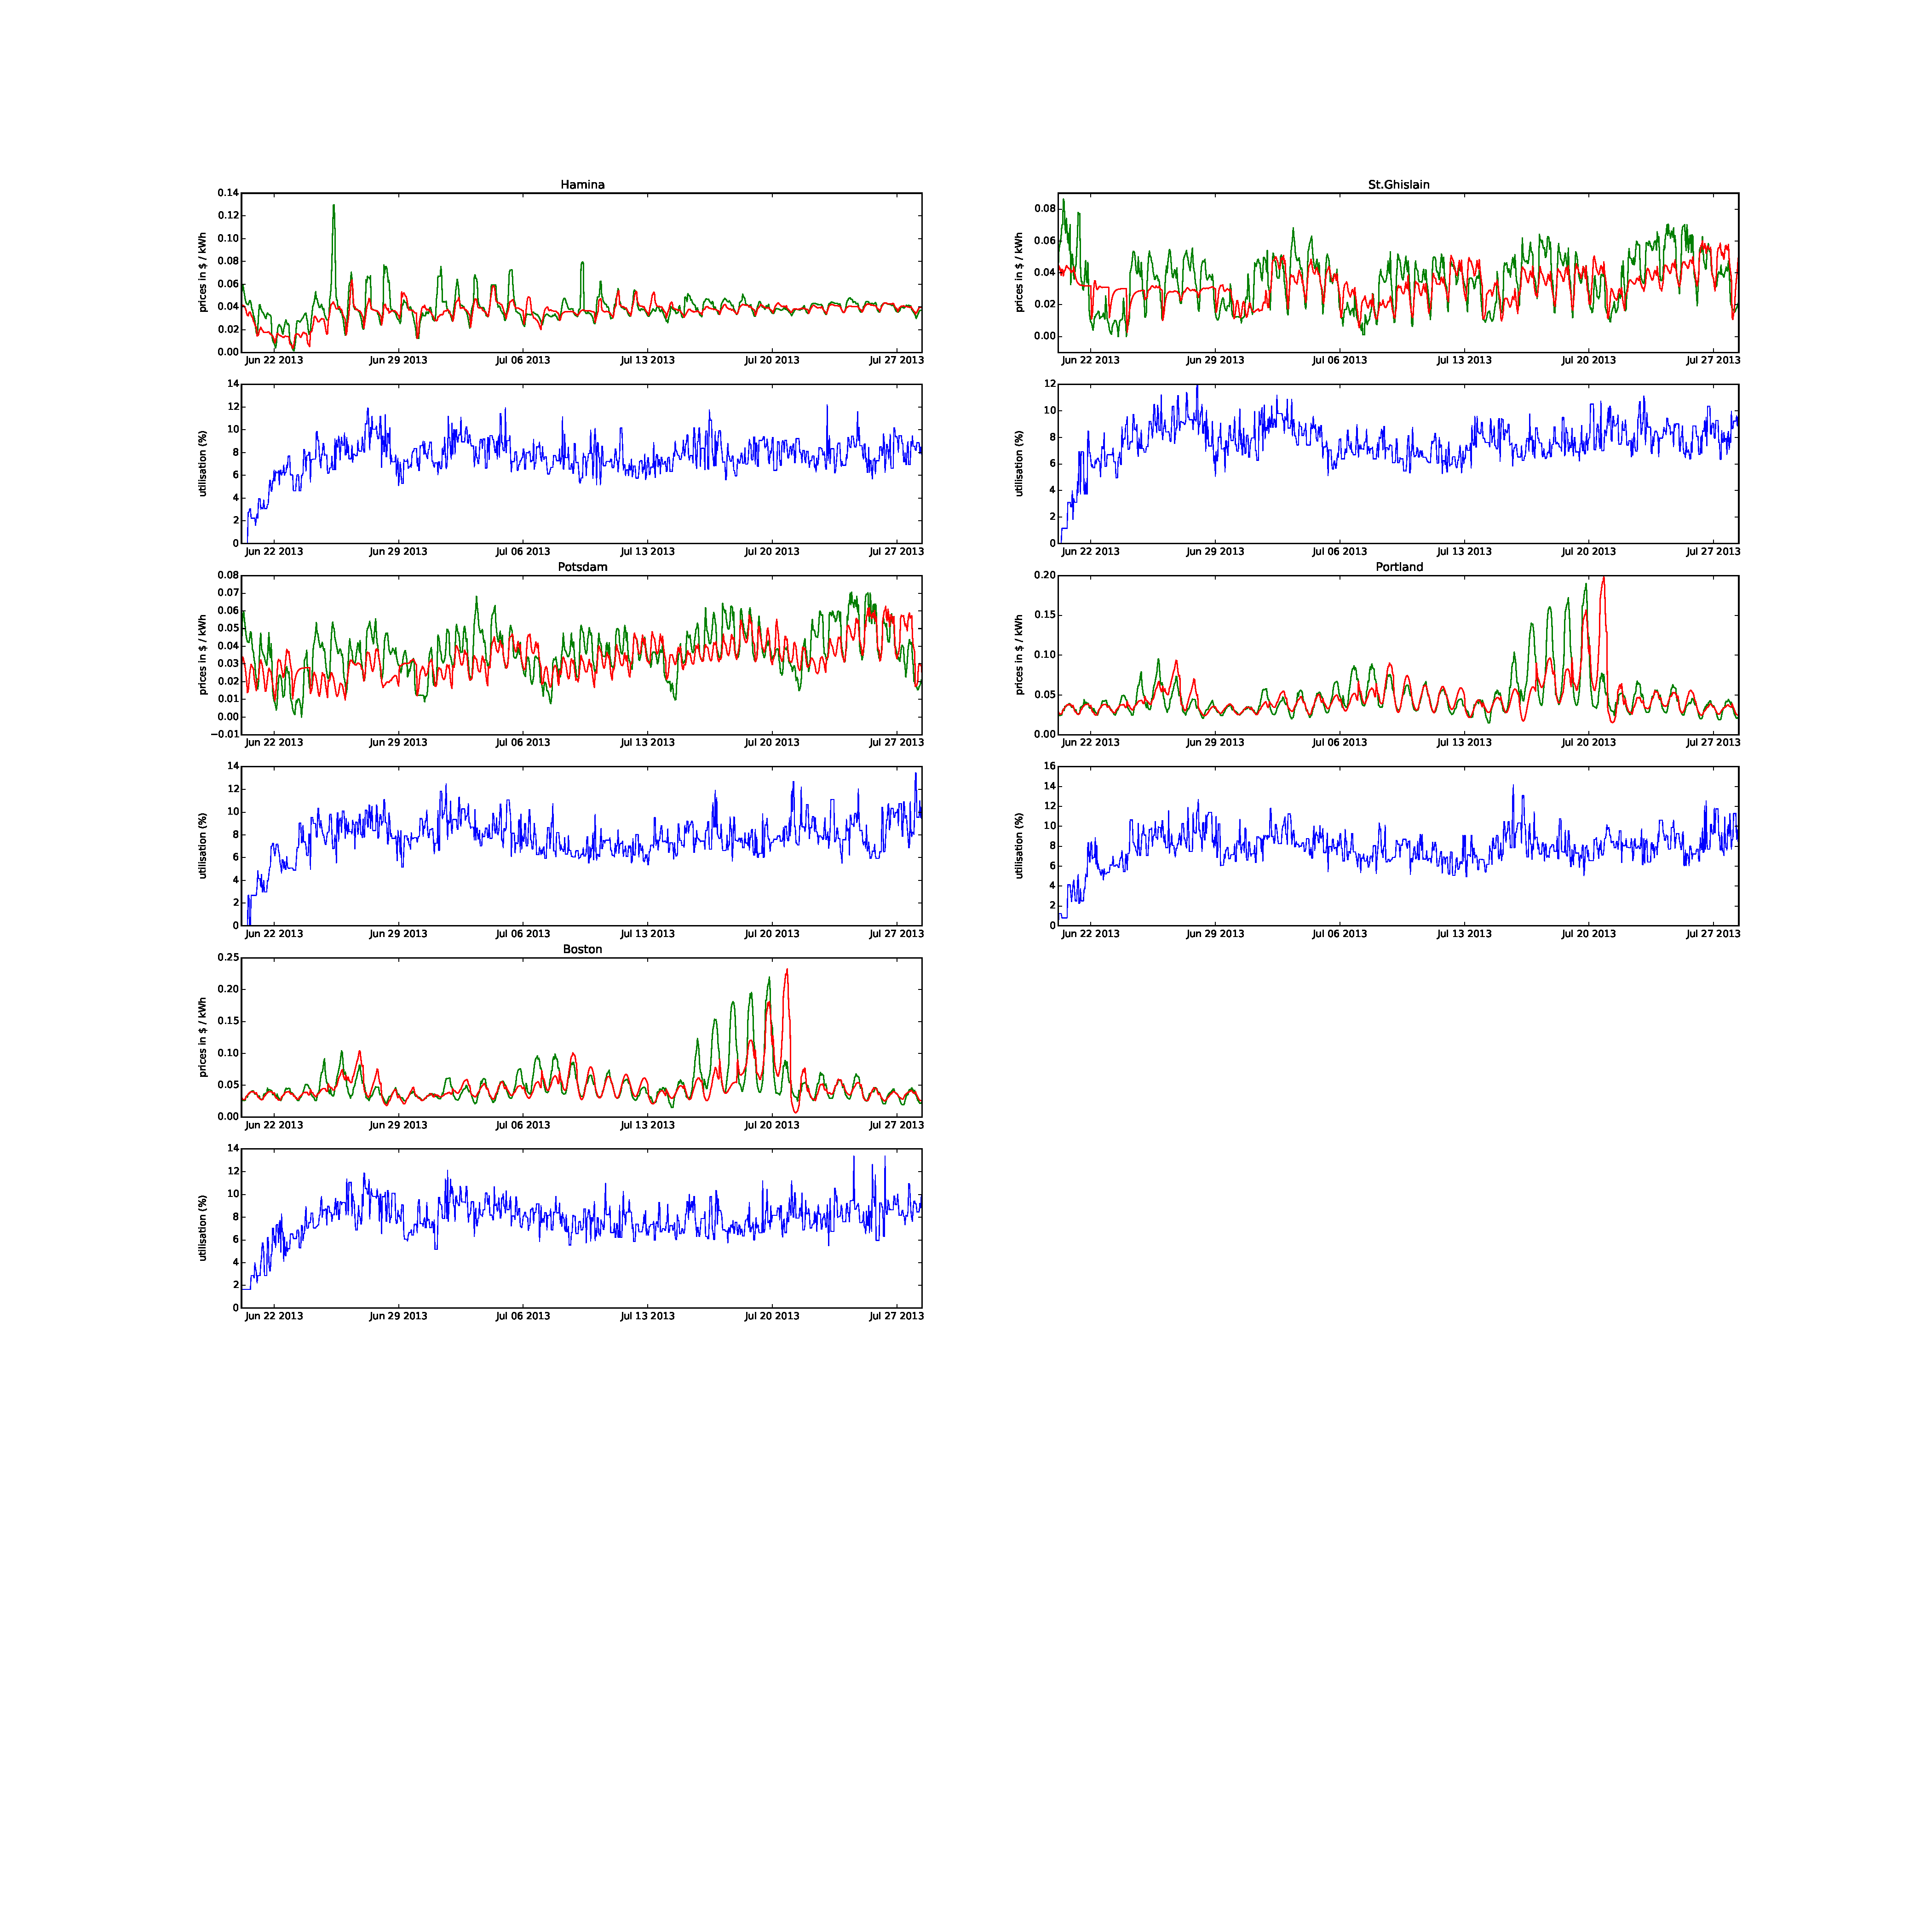
\includegraphics[width=1.60\textwidth]{figures/appendix_simulation_results/DA_Summer_scenario_1.pdf}
	\vspace*{-2.8in}
	\caption{Energy prices, energy price forecasts and utilization levels per location for simulation ``DA Summer'' and scheduler BFD}
	\label{fig:app_DA_Summer_scenario_1}
\end{figure}

\begin{figure}[htbp]
	\centering
	\vspace*{-0.6in}
	\hspace*{-1.9in}
		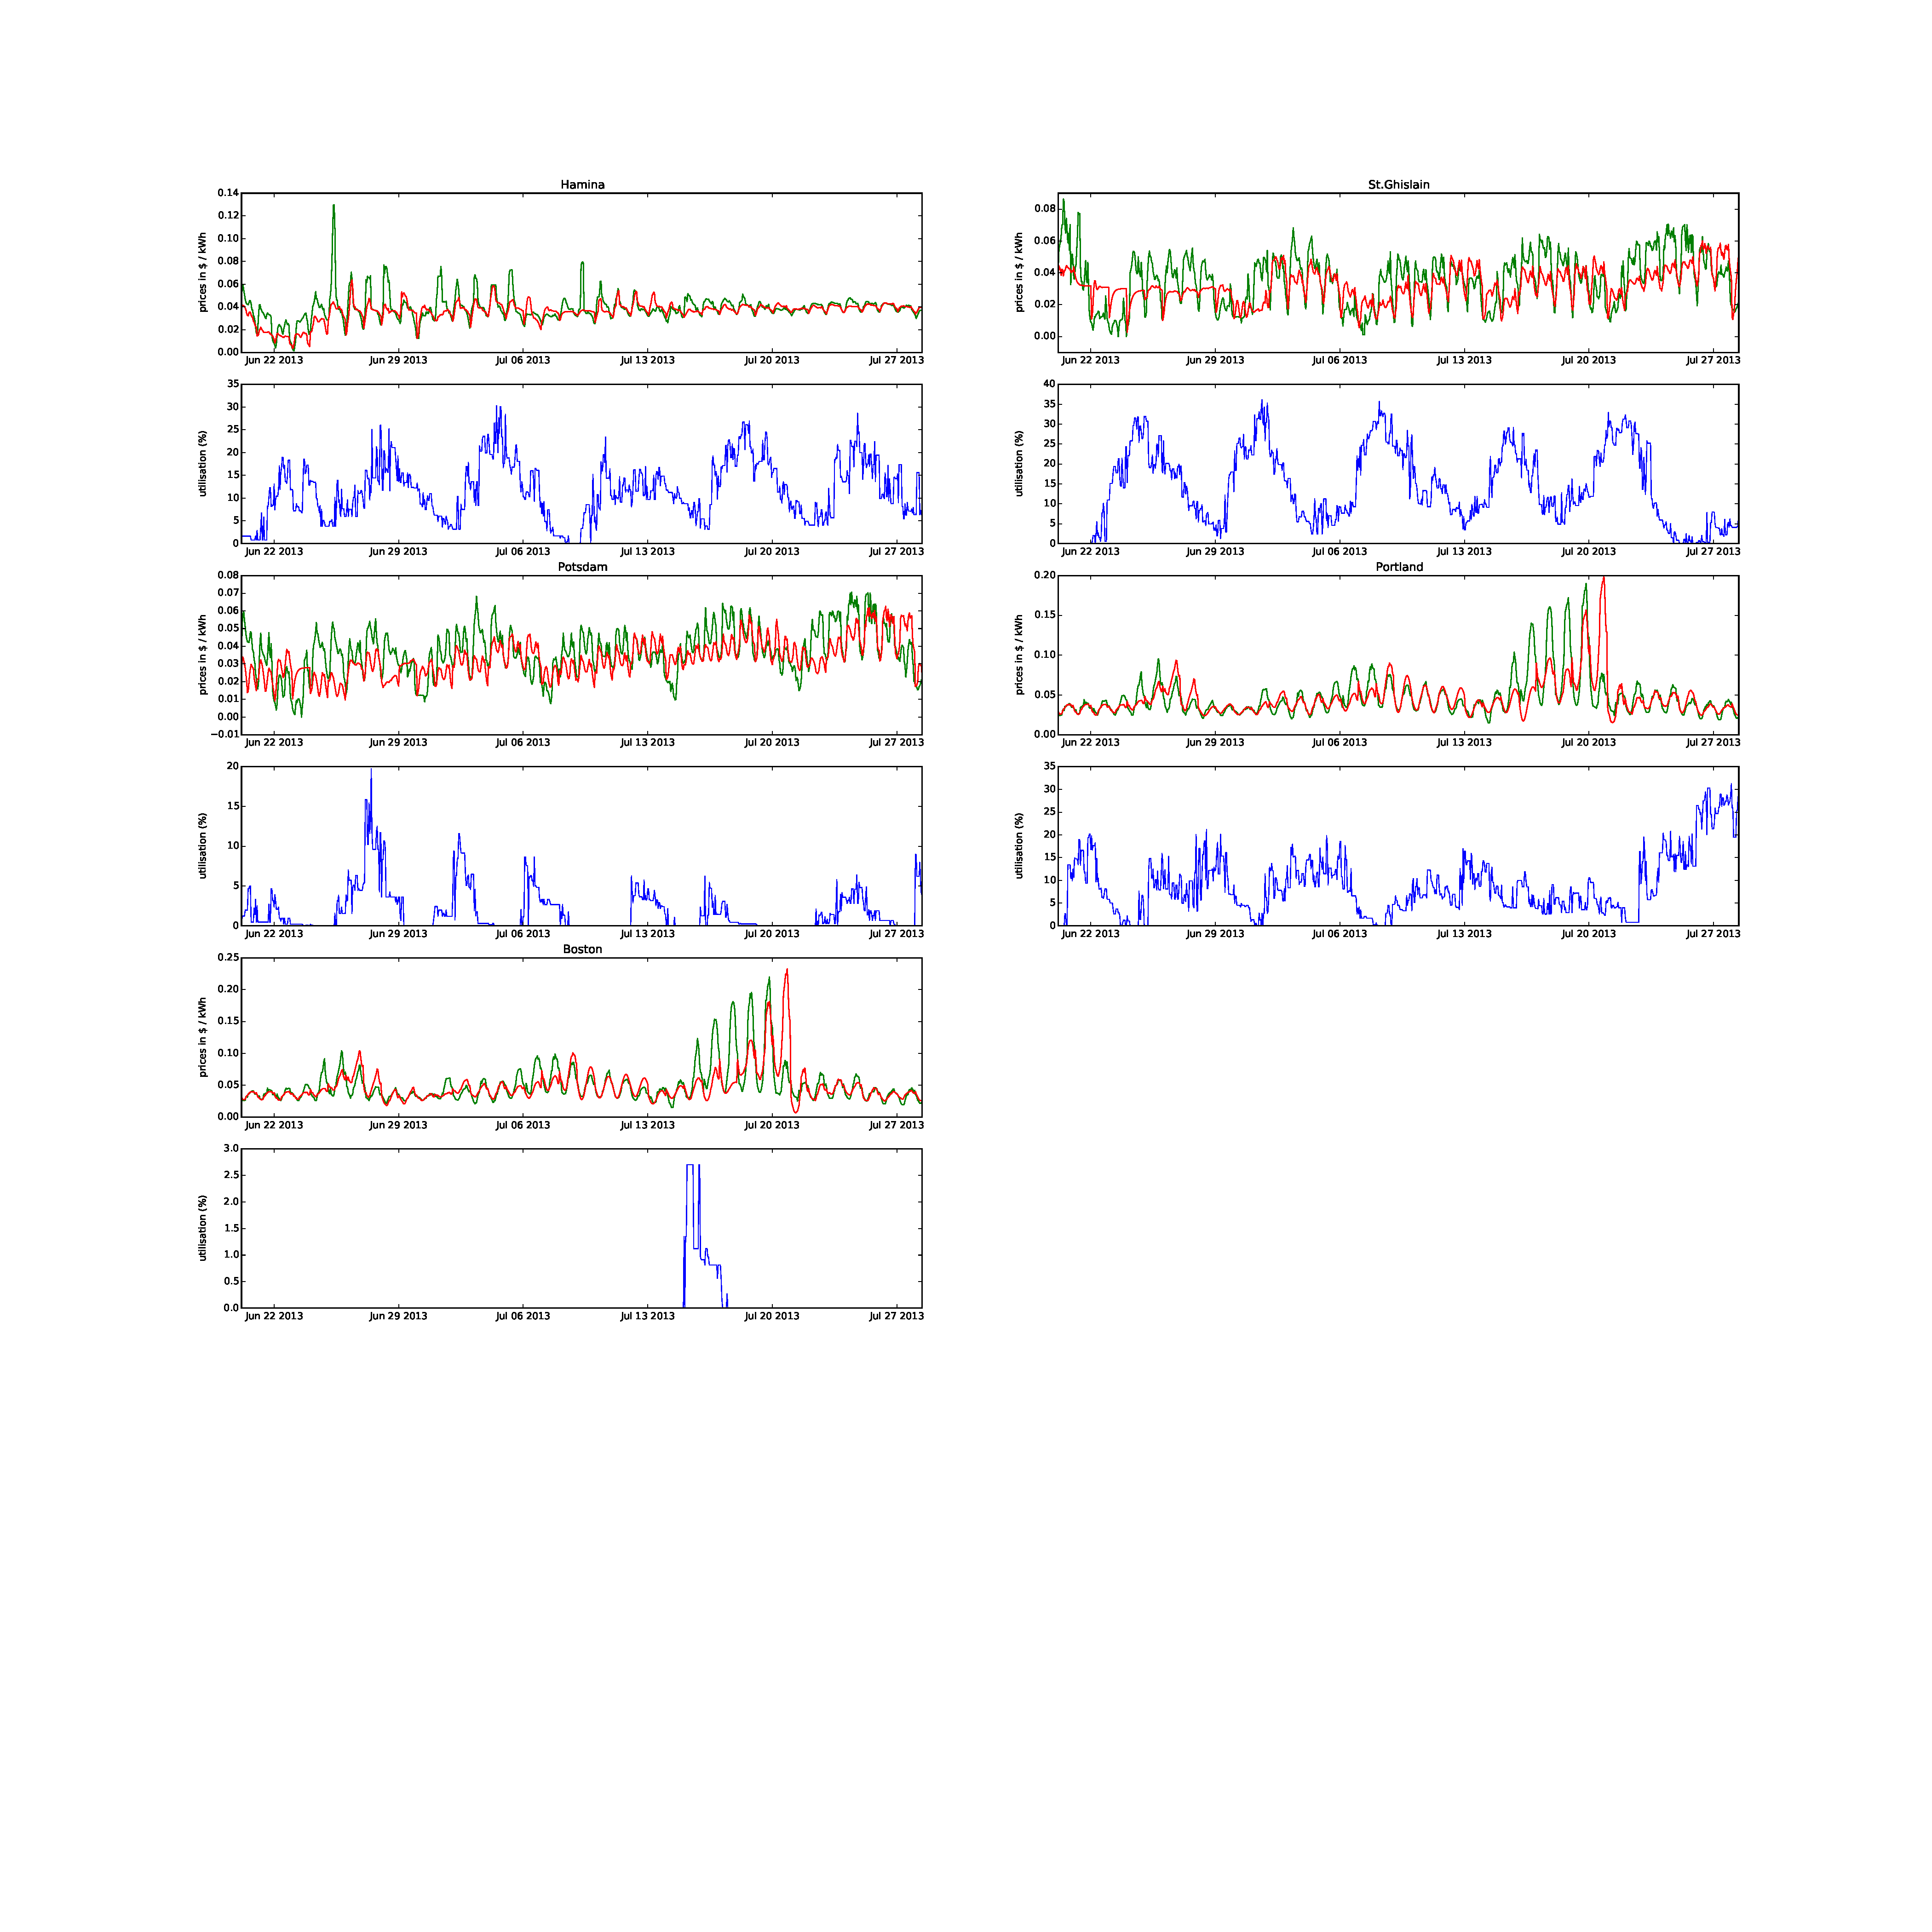
\includegraphics[width=1.60\textwidth]{figures/appendix_simulation_results/DA_Summer_scenario_2.pdf}
	\vspace*{-2.8in}
	\caption{Energy prices, energy price forecasts and utilization levels per location for simulation ``DA Summer'' and scheduler BCF}
	\label{fig:app_DA_Summer_scenario_2}
\end{figure}

\begin{figure}[htbp]
	\centering
	\vspace*{-0.6in}
	\hspace*{-1.4in}
		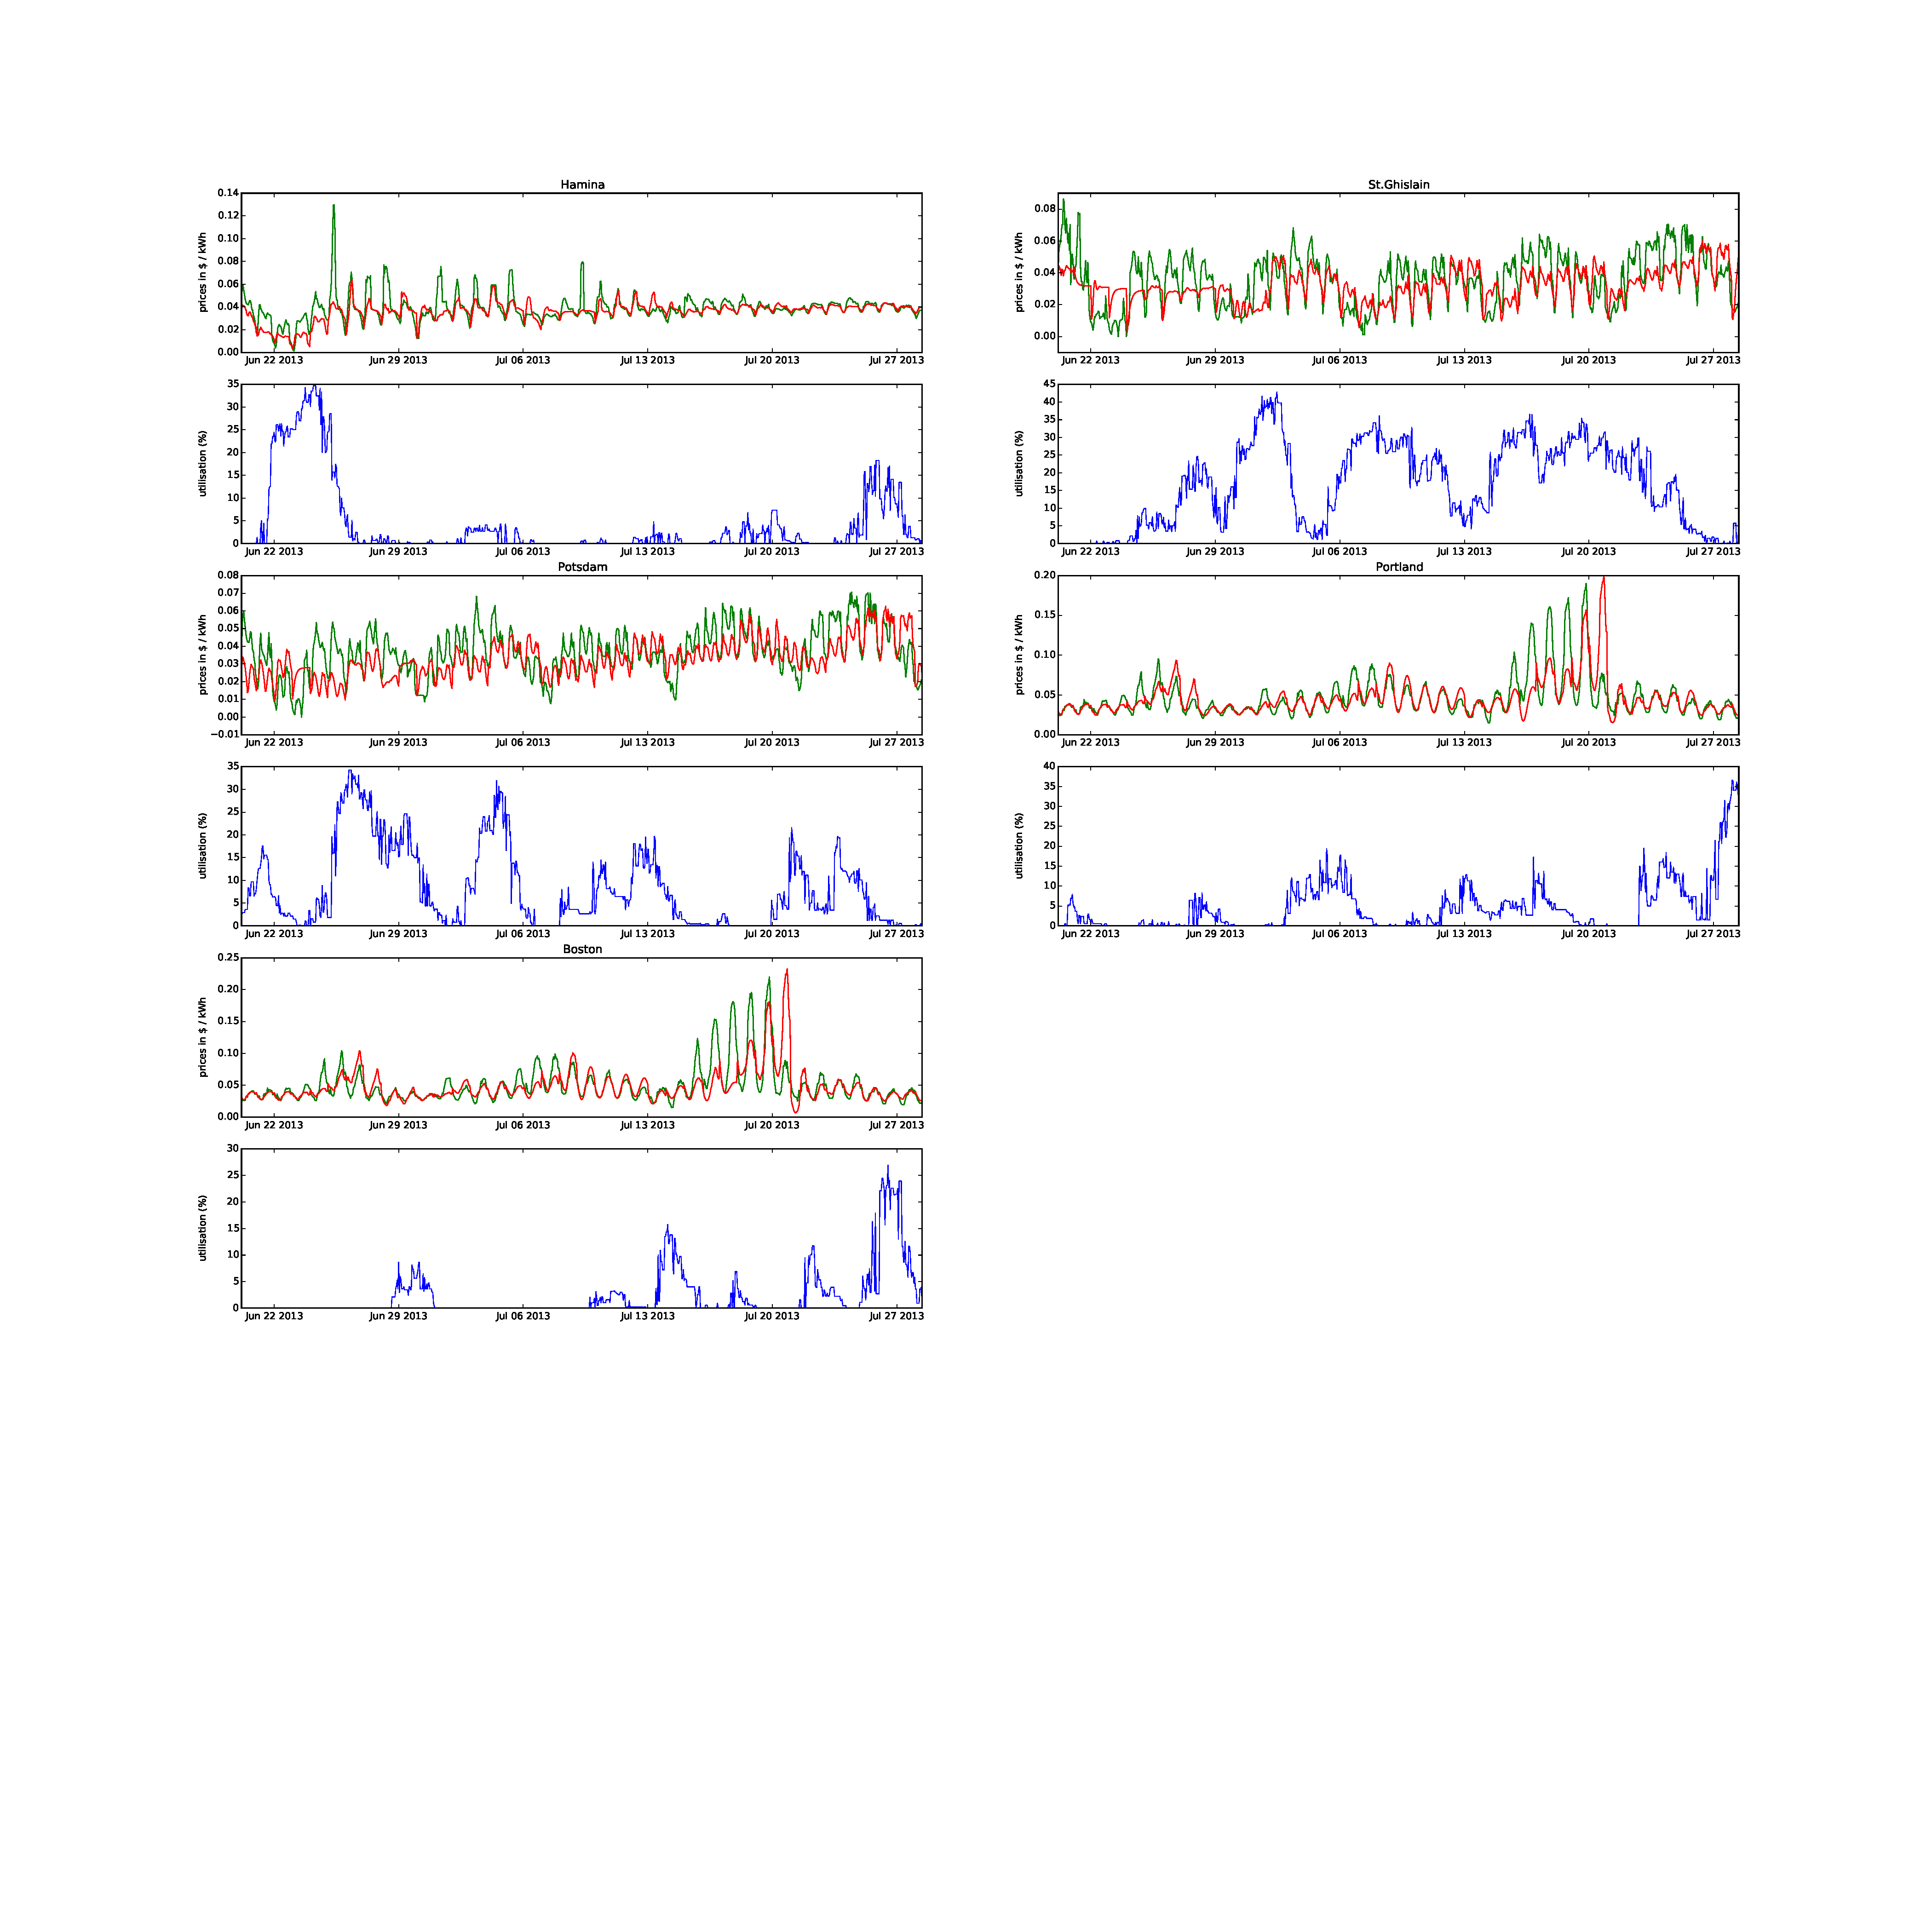
\includegraphics[width=1.60\textwidth]{figures/appendix_simulation_results/DA_Summer_scenario_3.pdf}
	\vspace*{-2.8in}
	\caption{Energy prices, energy price forecasts and utilization levels per location for simulation ``DA Summer'' and scheduler BCF\_F}
	\label{fig:app_DA_Summer_scenario_3}
\end{figure}

\begin{figure}[htbp]
	\centering
	\vspace*{-0.6in}
	\hspace*{-1.9in}
		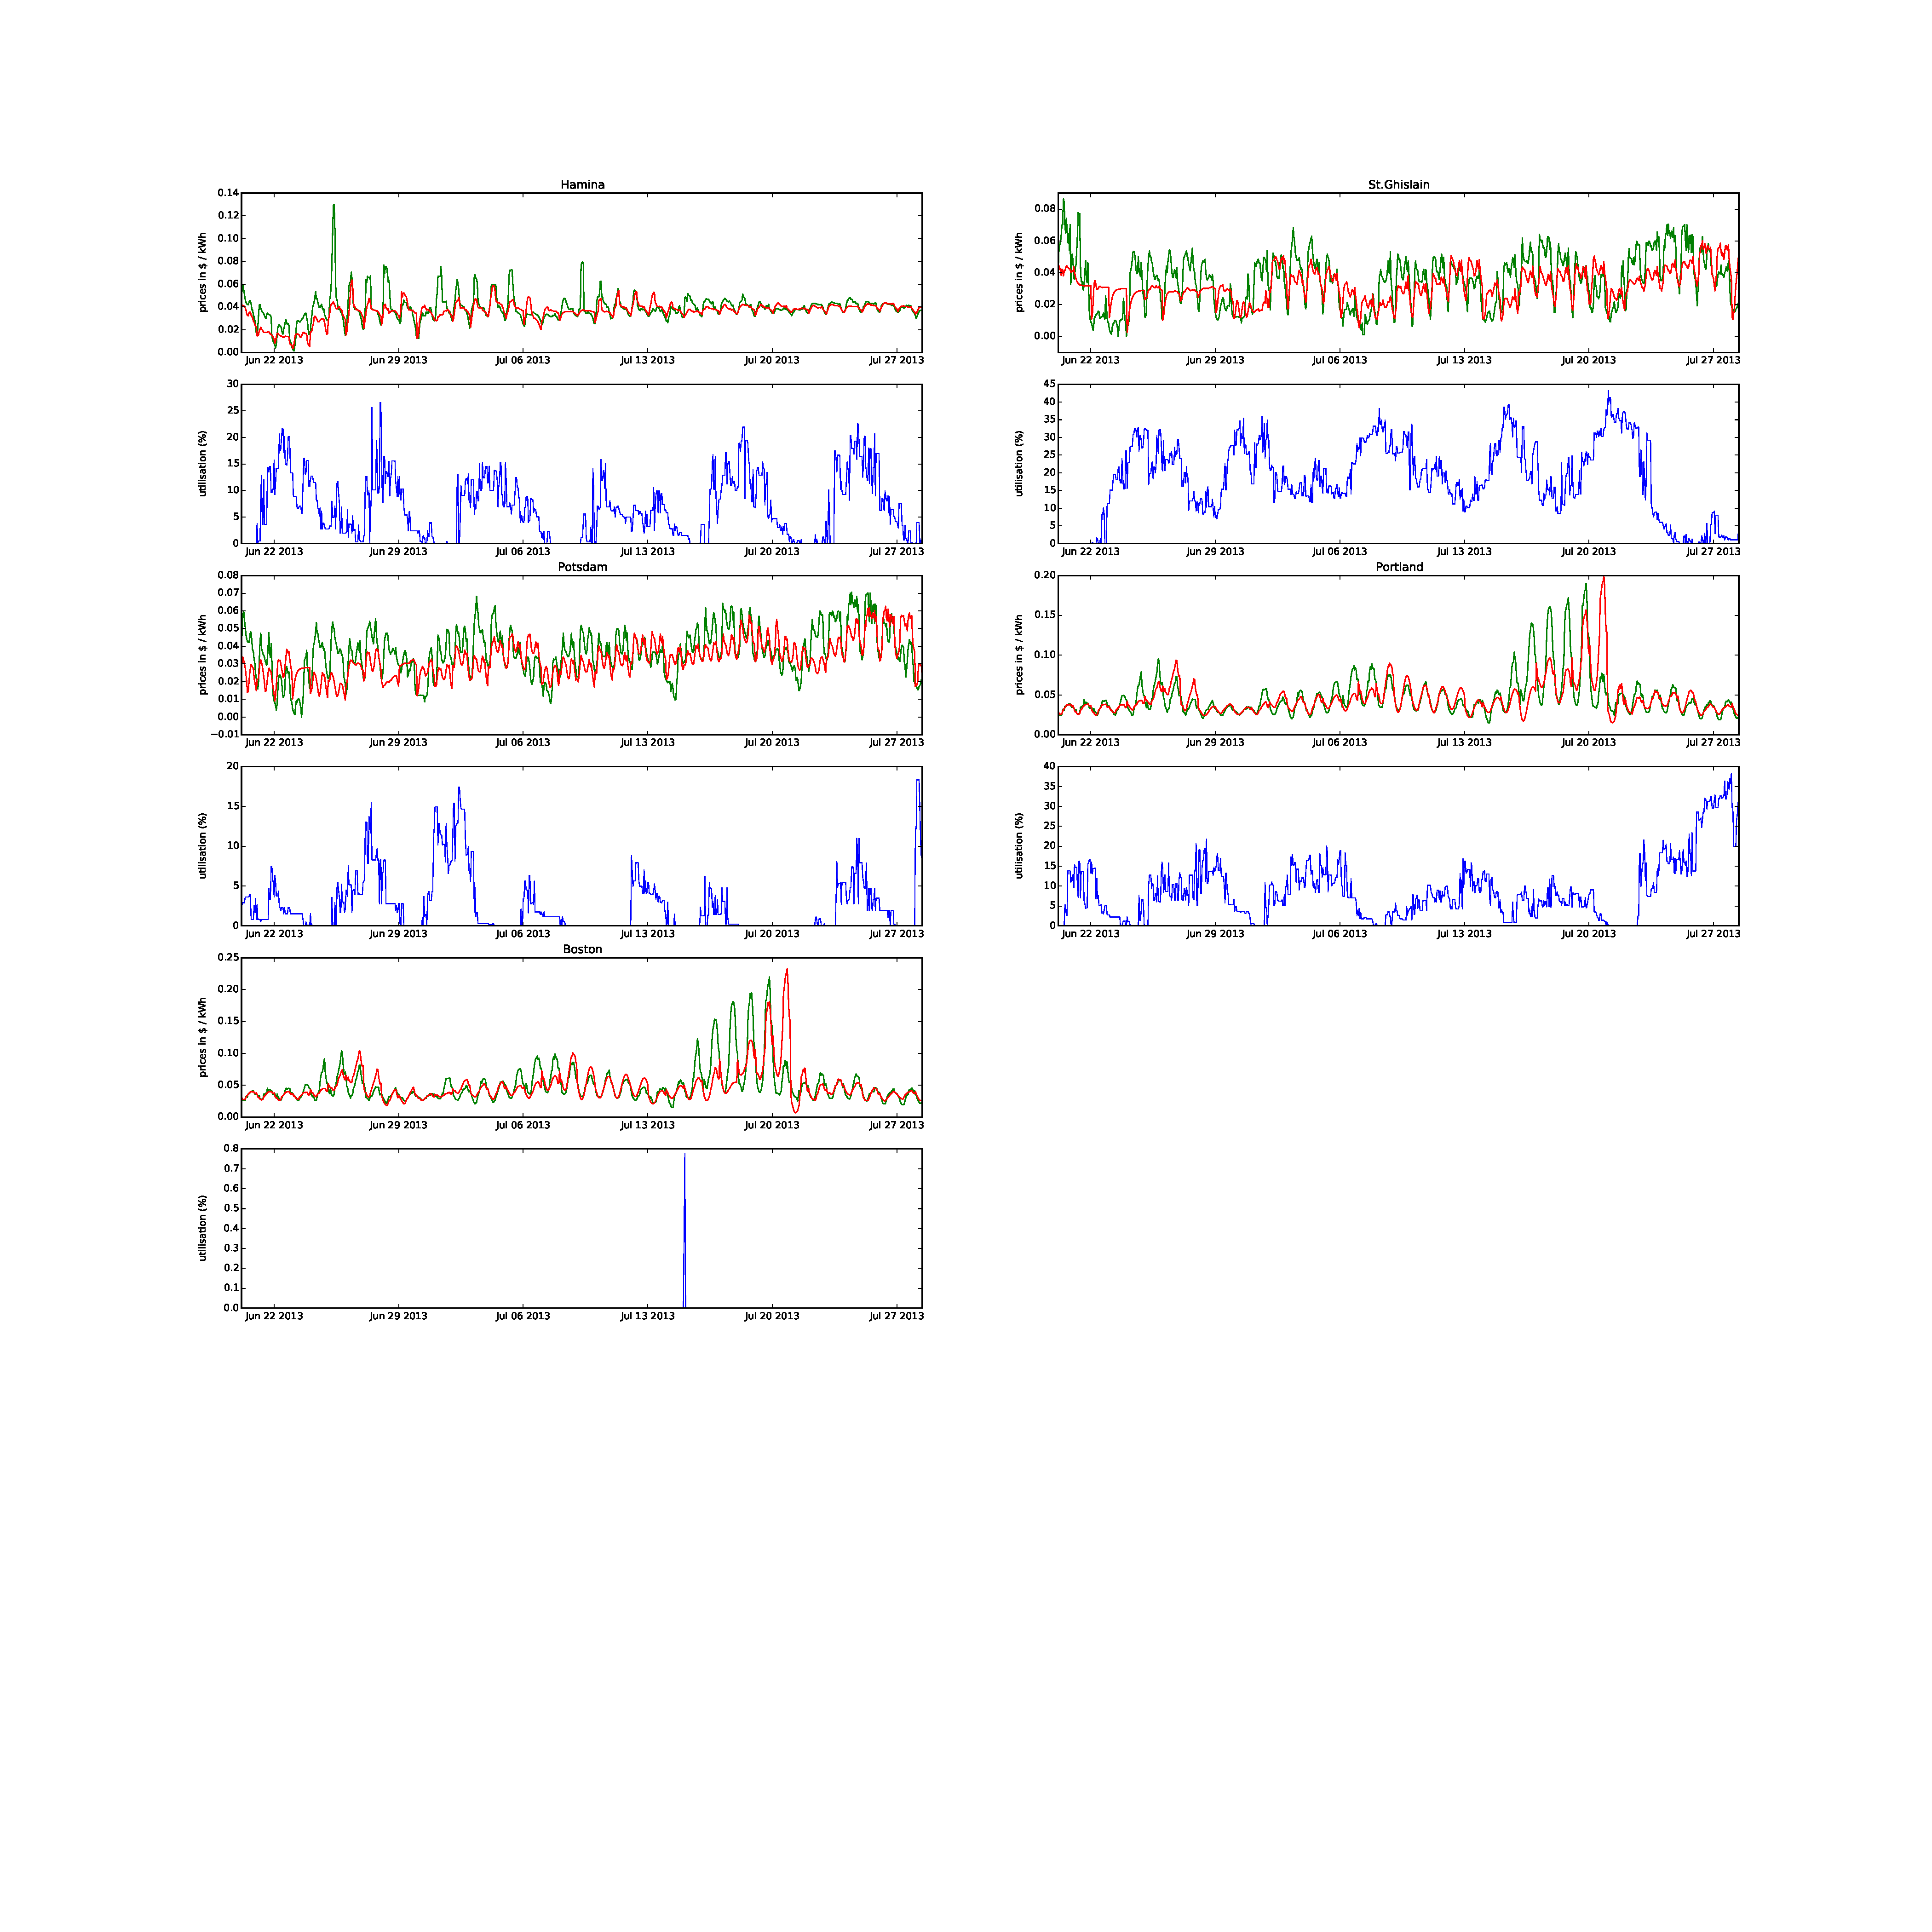
\includegraphics[width=1.60\textwidth]{figures/appendix_simulation_results/DA_Summer_scenario_4.pdf}
	\vspace*{-2.8in}
	\caption{Energy prices, energy price forecasts and utilization levels per location for simulation ``DA Summer'' and scheduler BCF\_IF}
	\label{fig:app_DA_Summer_scenario_4}
\end{figure}

\begin{figure}[htbp]
	\centering
	\vspace*{-0.6in}
	\hspace*{-1.4in}
		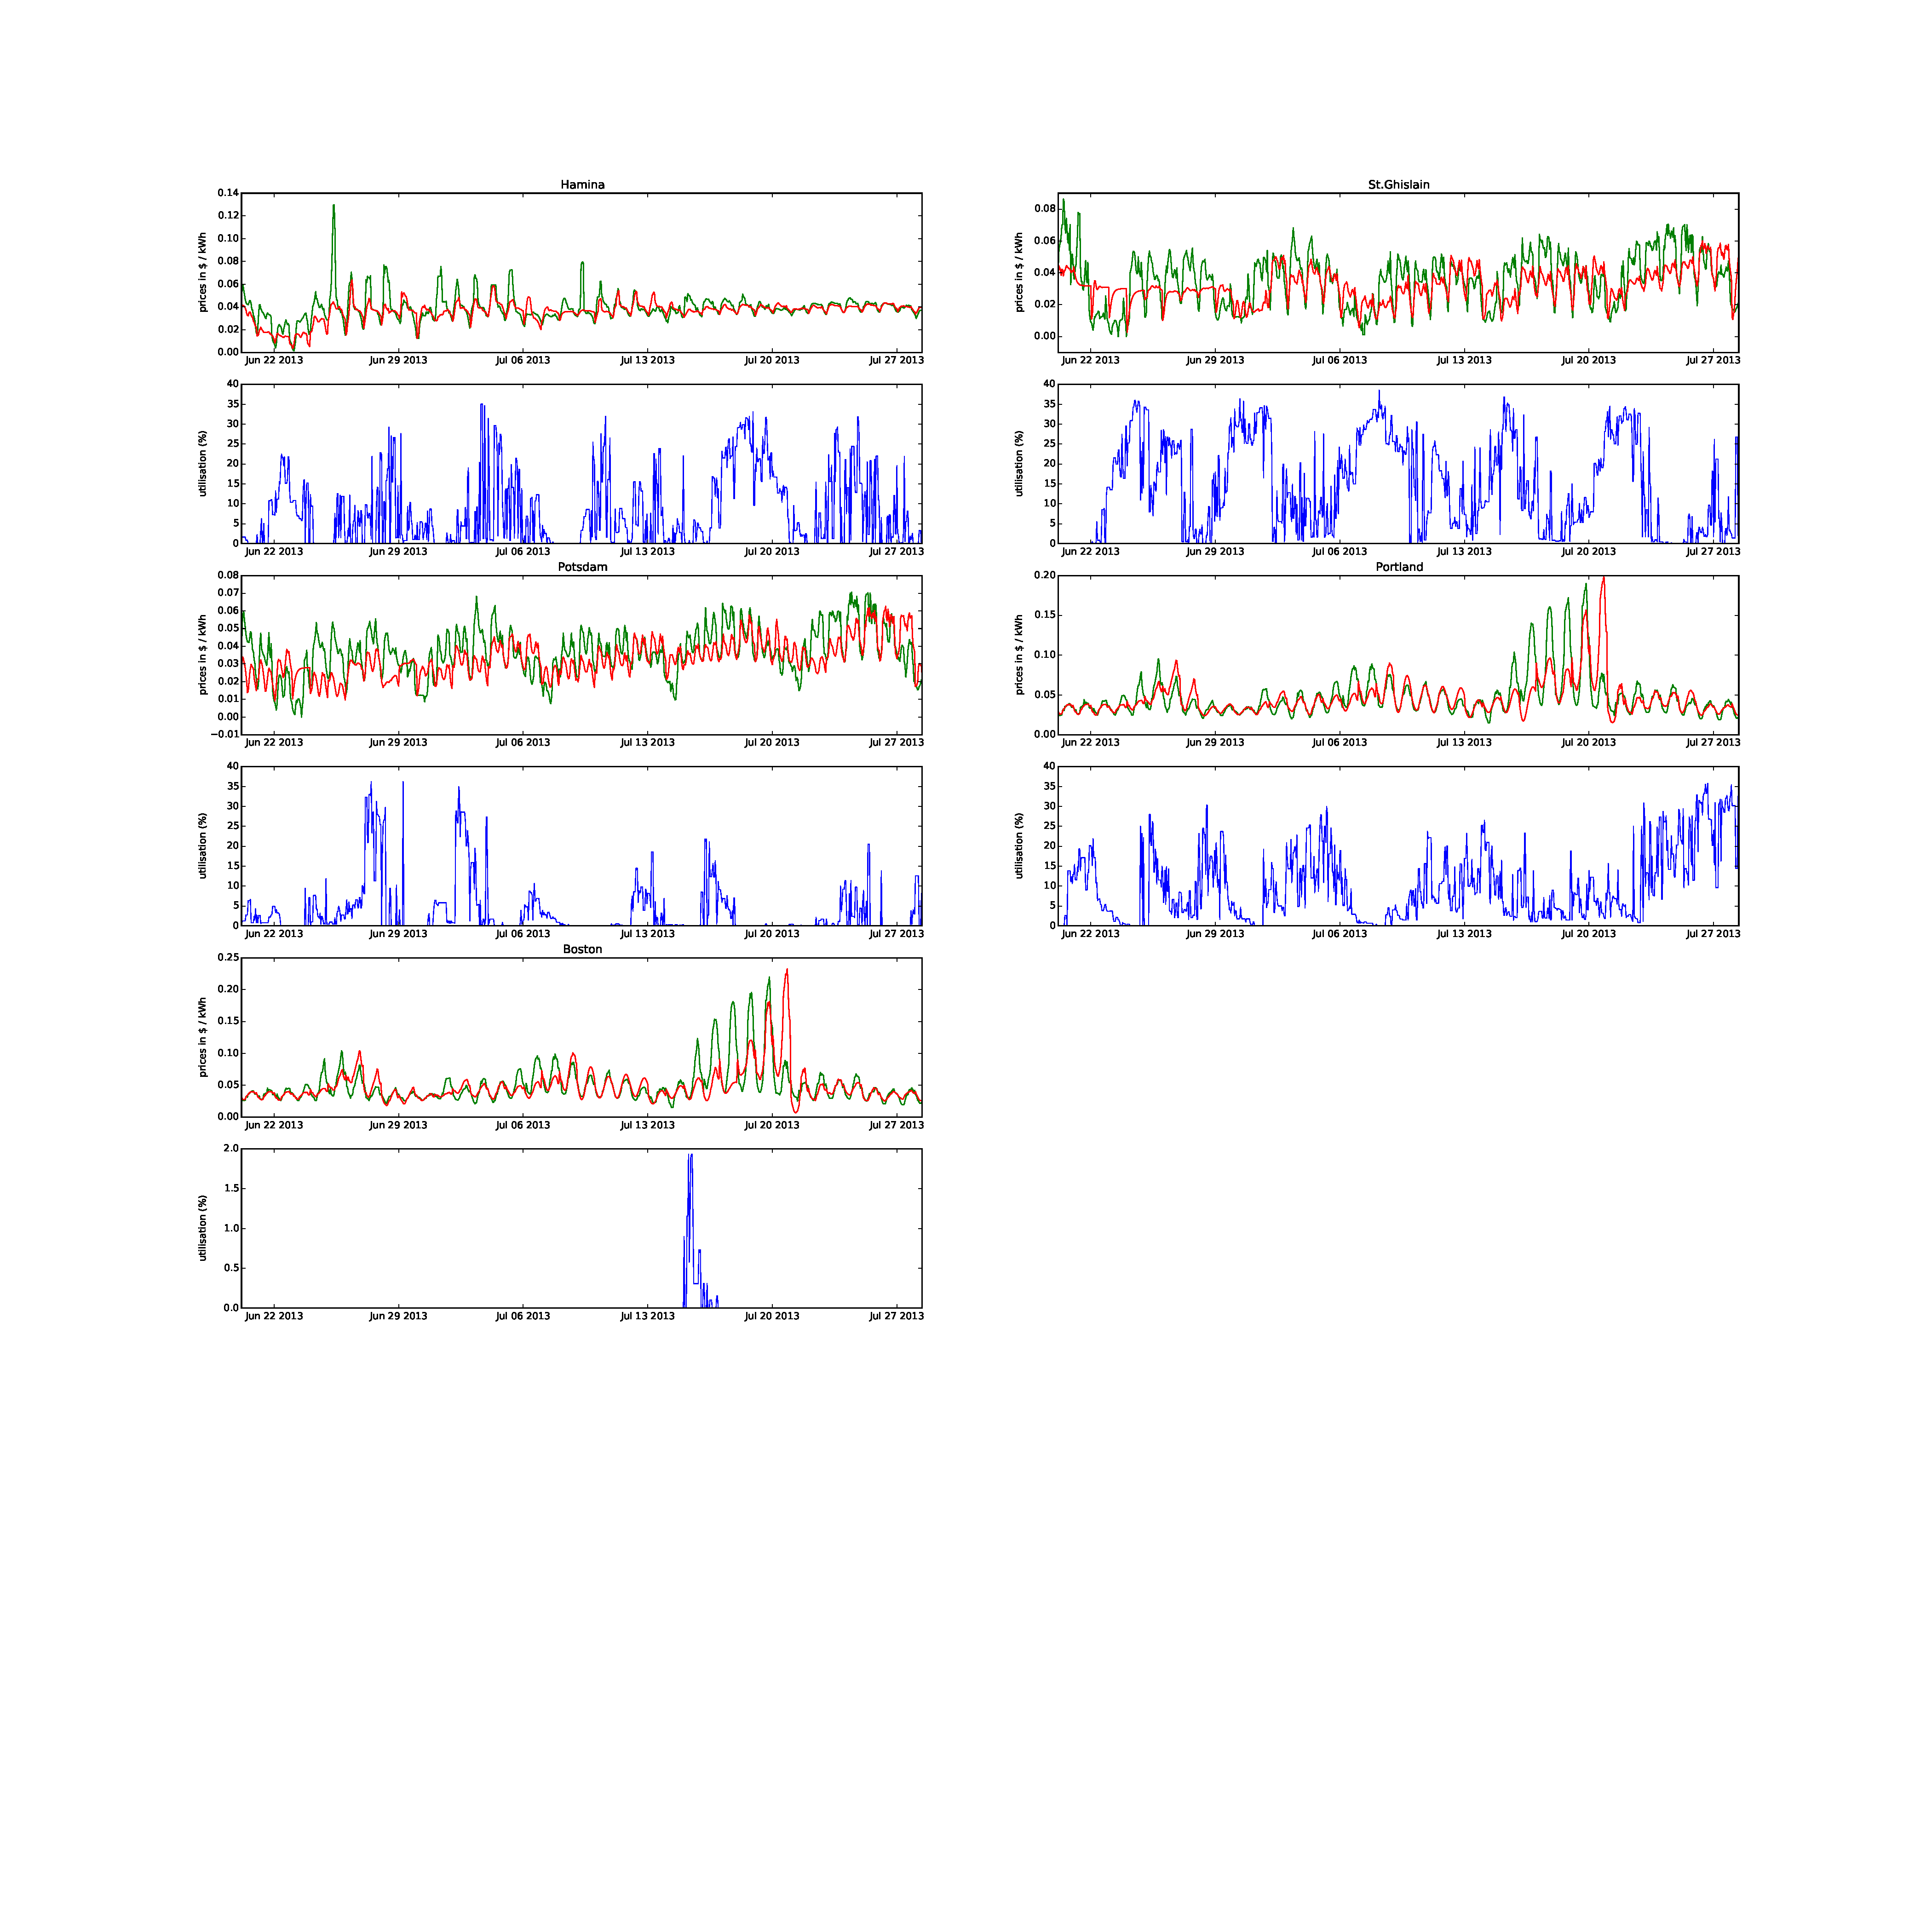
\includegraphics[width=1.60\textwidth]{figures/appendix_simulation_results/DA_Summer_scenario_5.pdf}
	\vspace*{-2.8in}
	\caption{Energy prices, energy price forecasts and utilization levels per location for simulation ``DA Summer'' and scheduler BCU\_M}
	\label{fig:app_DA_Summer_scenario_5}
\end{figure}

\begin{figure}[htbp]
	\centering
	\vspace*{-0.6in}
	\hspace*{-1.9in}
		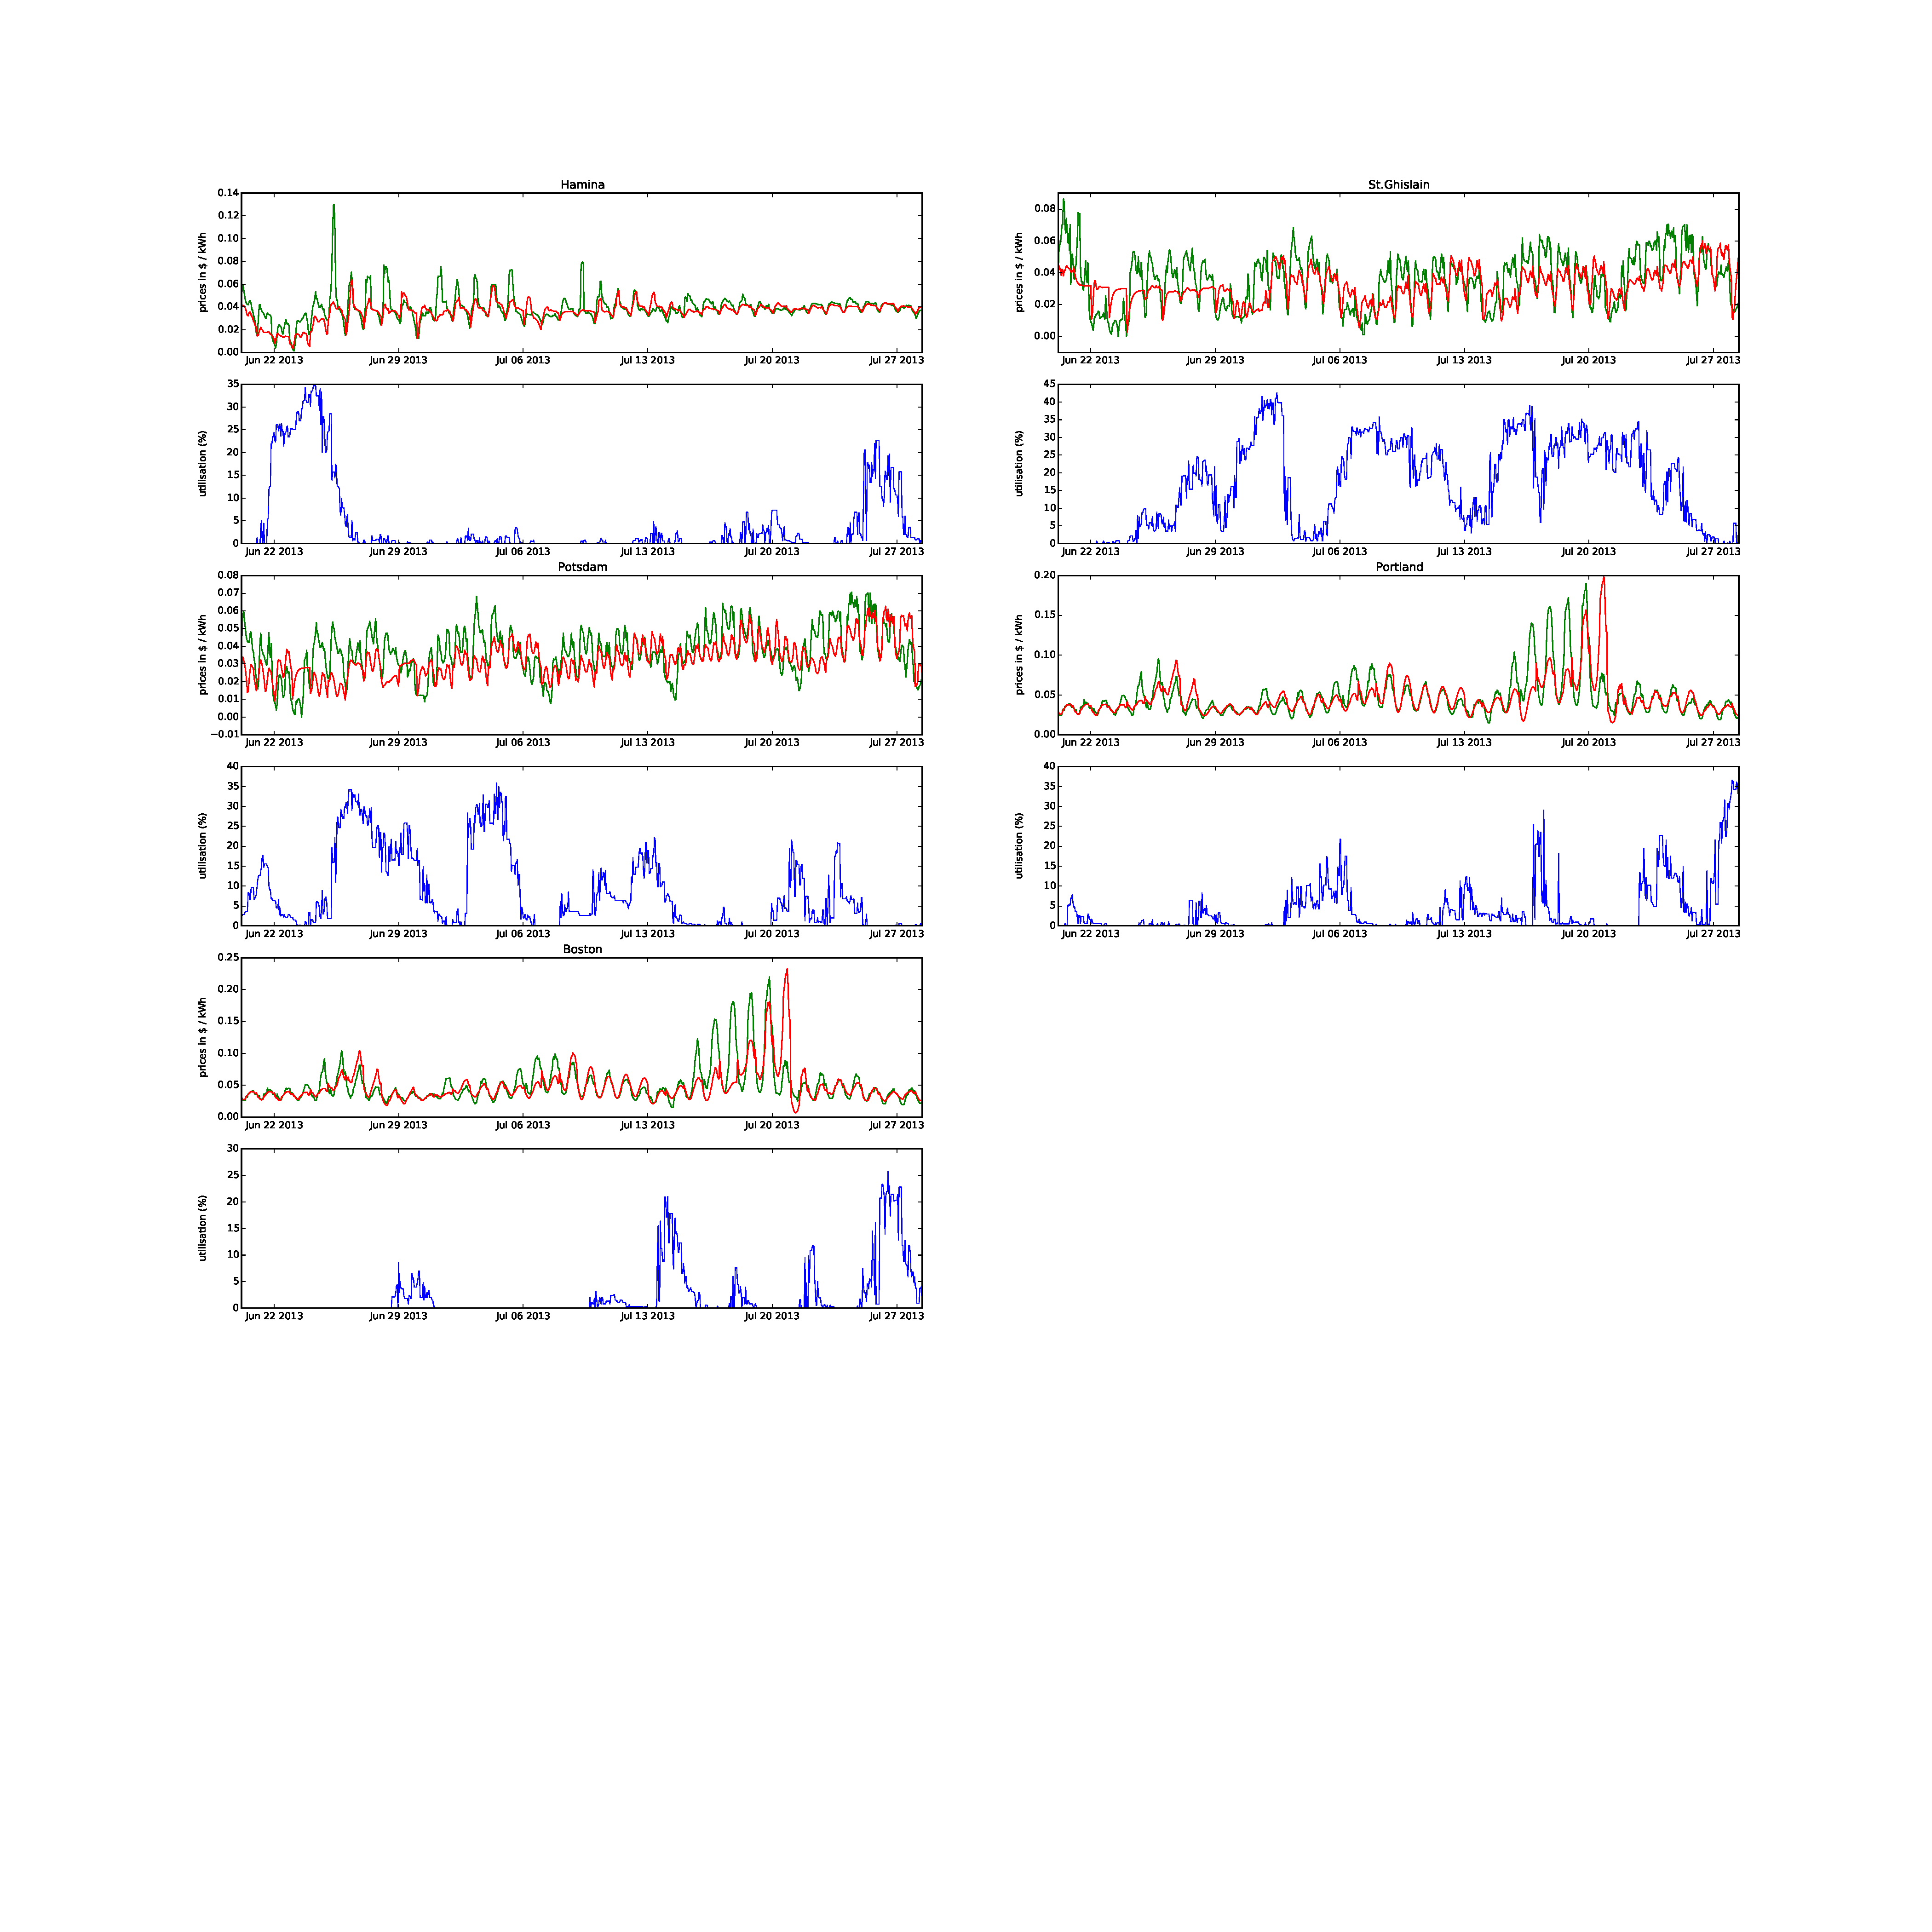
\includegraphics[width=1.60\textwidth]{figures/appendix_simulation_results/DA_Summer_scenario_6.pdf}
	\vspace*{-2.8in}
	\caption{Energy prices, energy price forecasts and utilization levels per location for simulation ``DA Summer'' and scheduler BCU\_MF}
	\label{fig:app_DA_Summer_scenario_6}
\end{figure}

\begin{figure}[htbp]
	\centering
	\vspace*{-0.6in}
	\hspace*{-1.4in}
		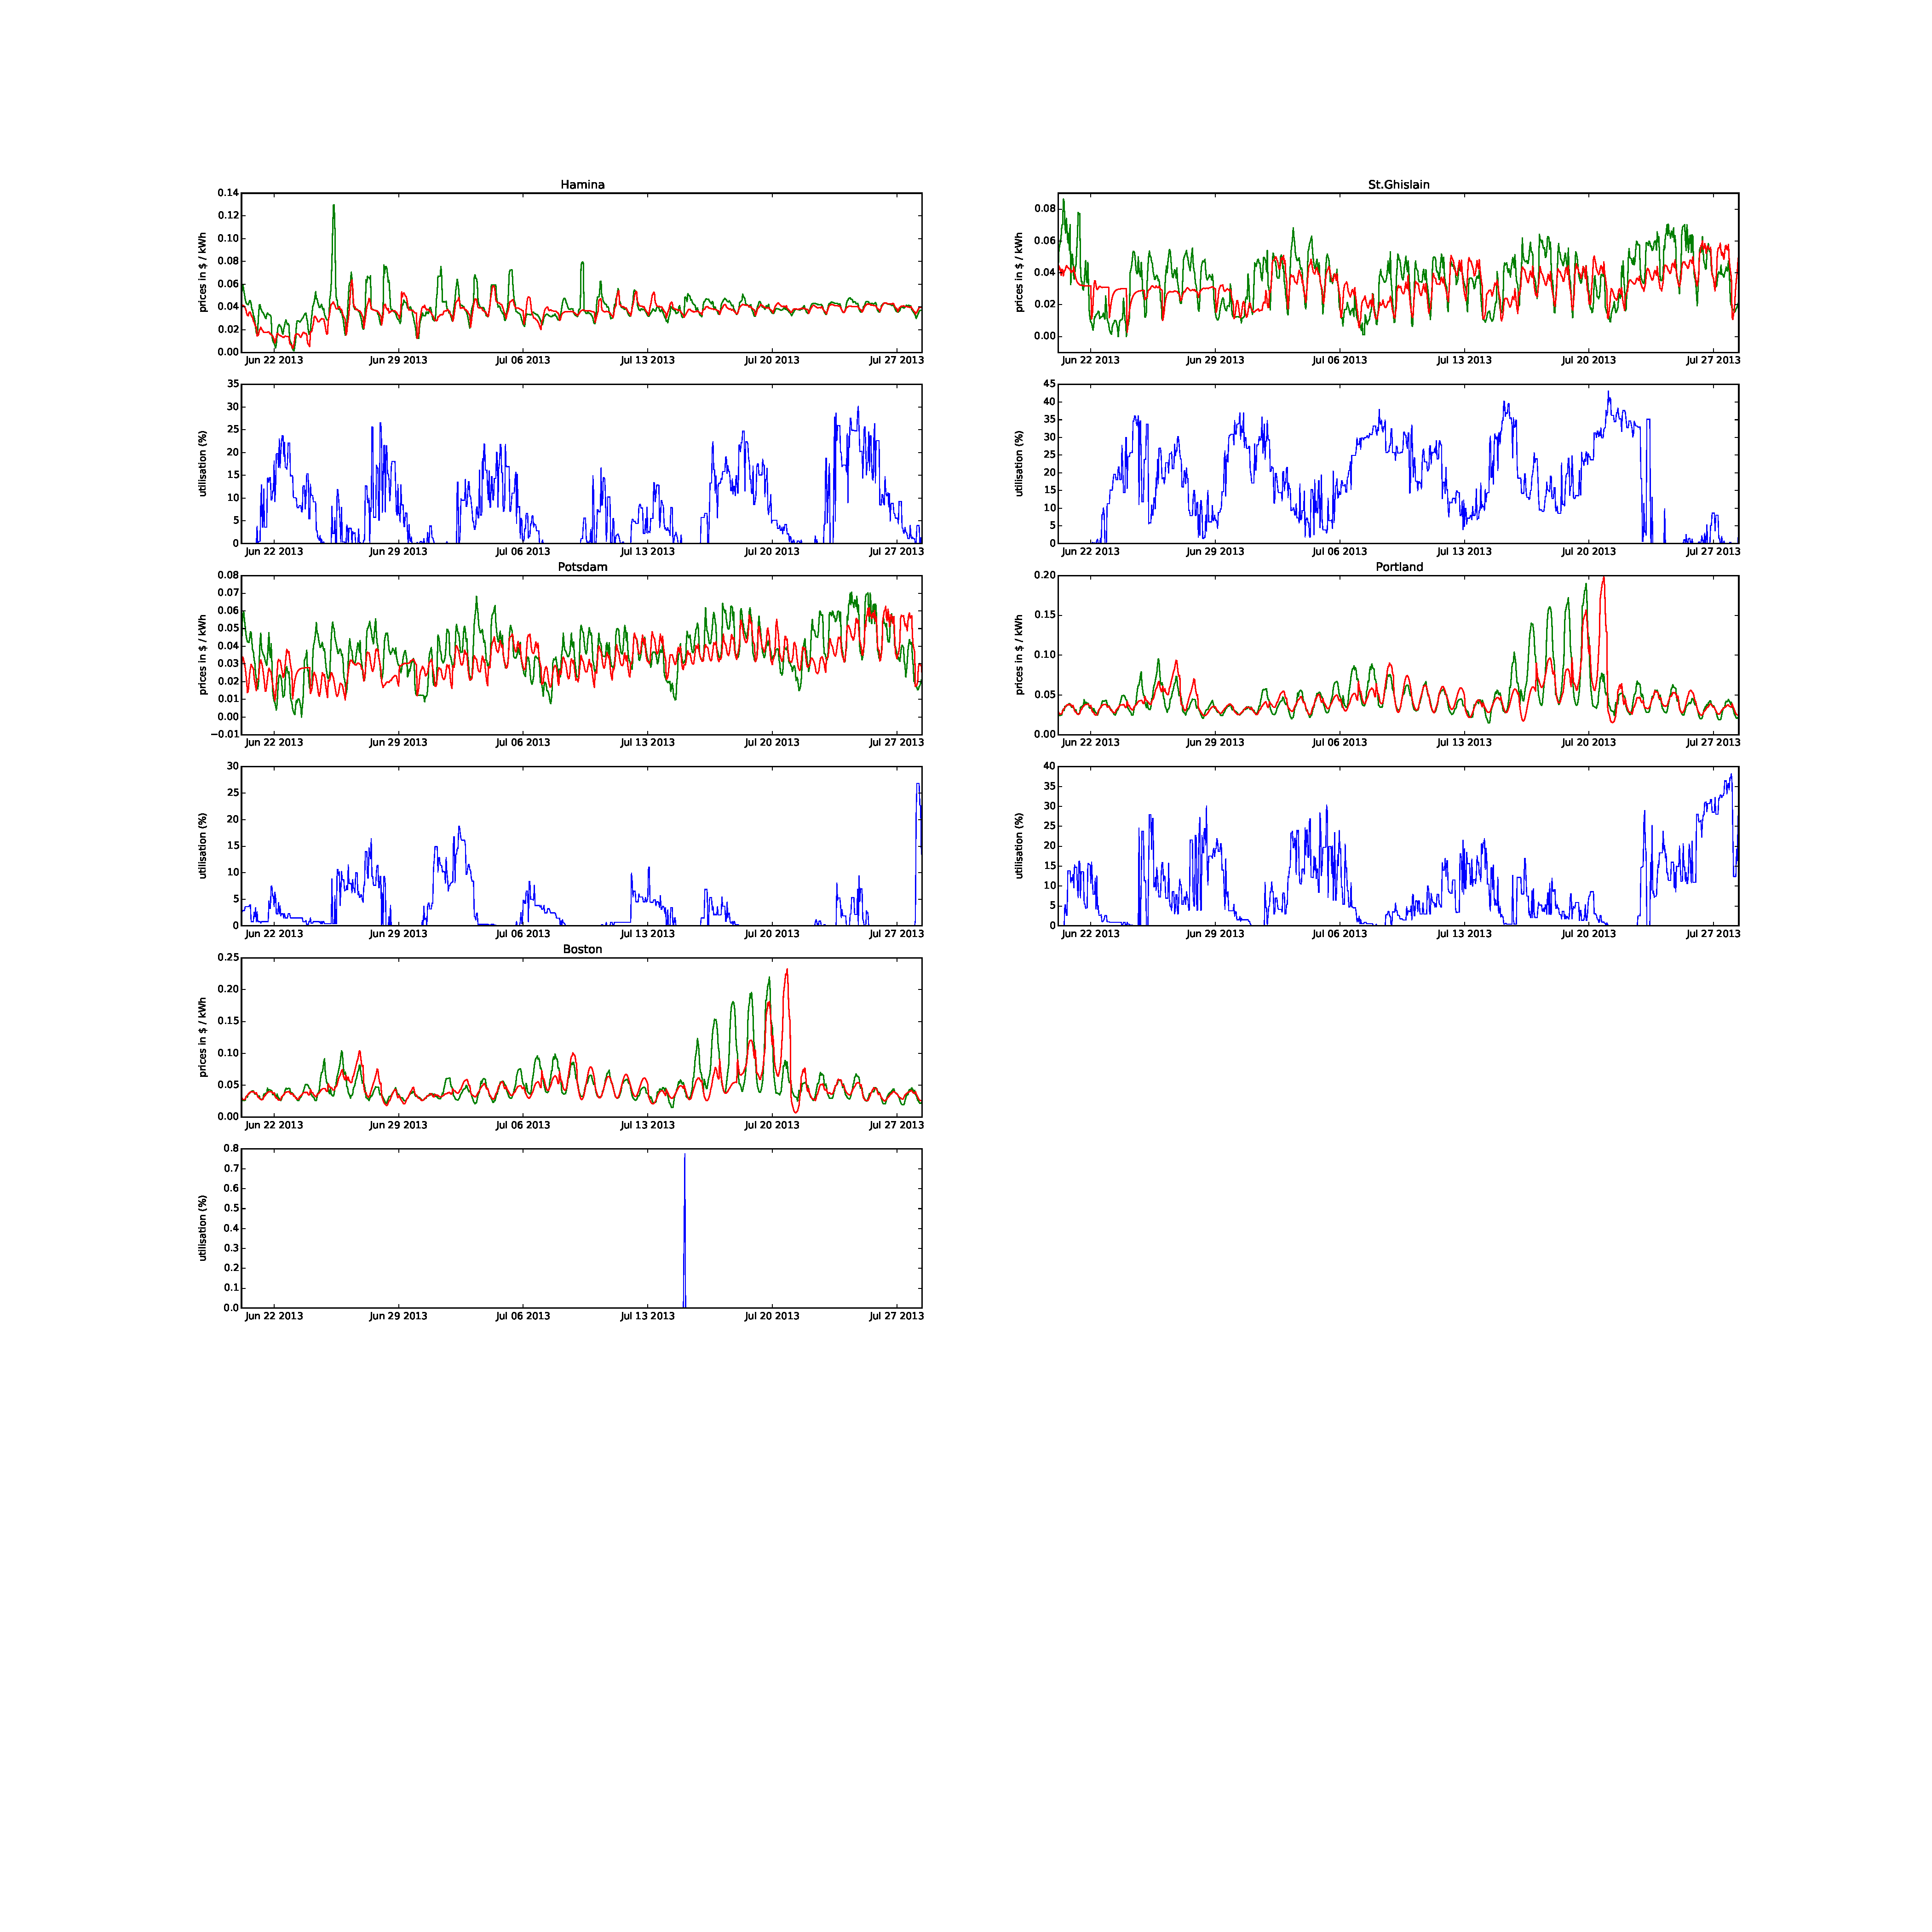
\includegraphics[width=1.60\textwidth]{figures/appendix_simulation_results/DA_Summer_scenario_7.pdf}
	\vspace*{-2.8in}
	\caption{Energy prices, energy price forecasts and utilization levels per location for simulation ``DA Summer'' and scheduler BCU\_MIF}
	\label{fig:app_DA_Summer_scenario_7}
\end{figure}


\FloatBarrier
\subsection{Simulation results for DA Spring}

\newpage

\begin{figure}[htbp]
	\centering
	\vspace*{-0.6in}
	\hspace*{-1.4in}
		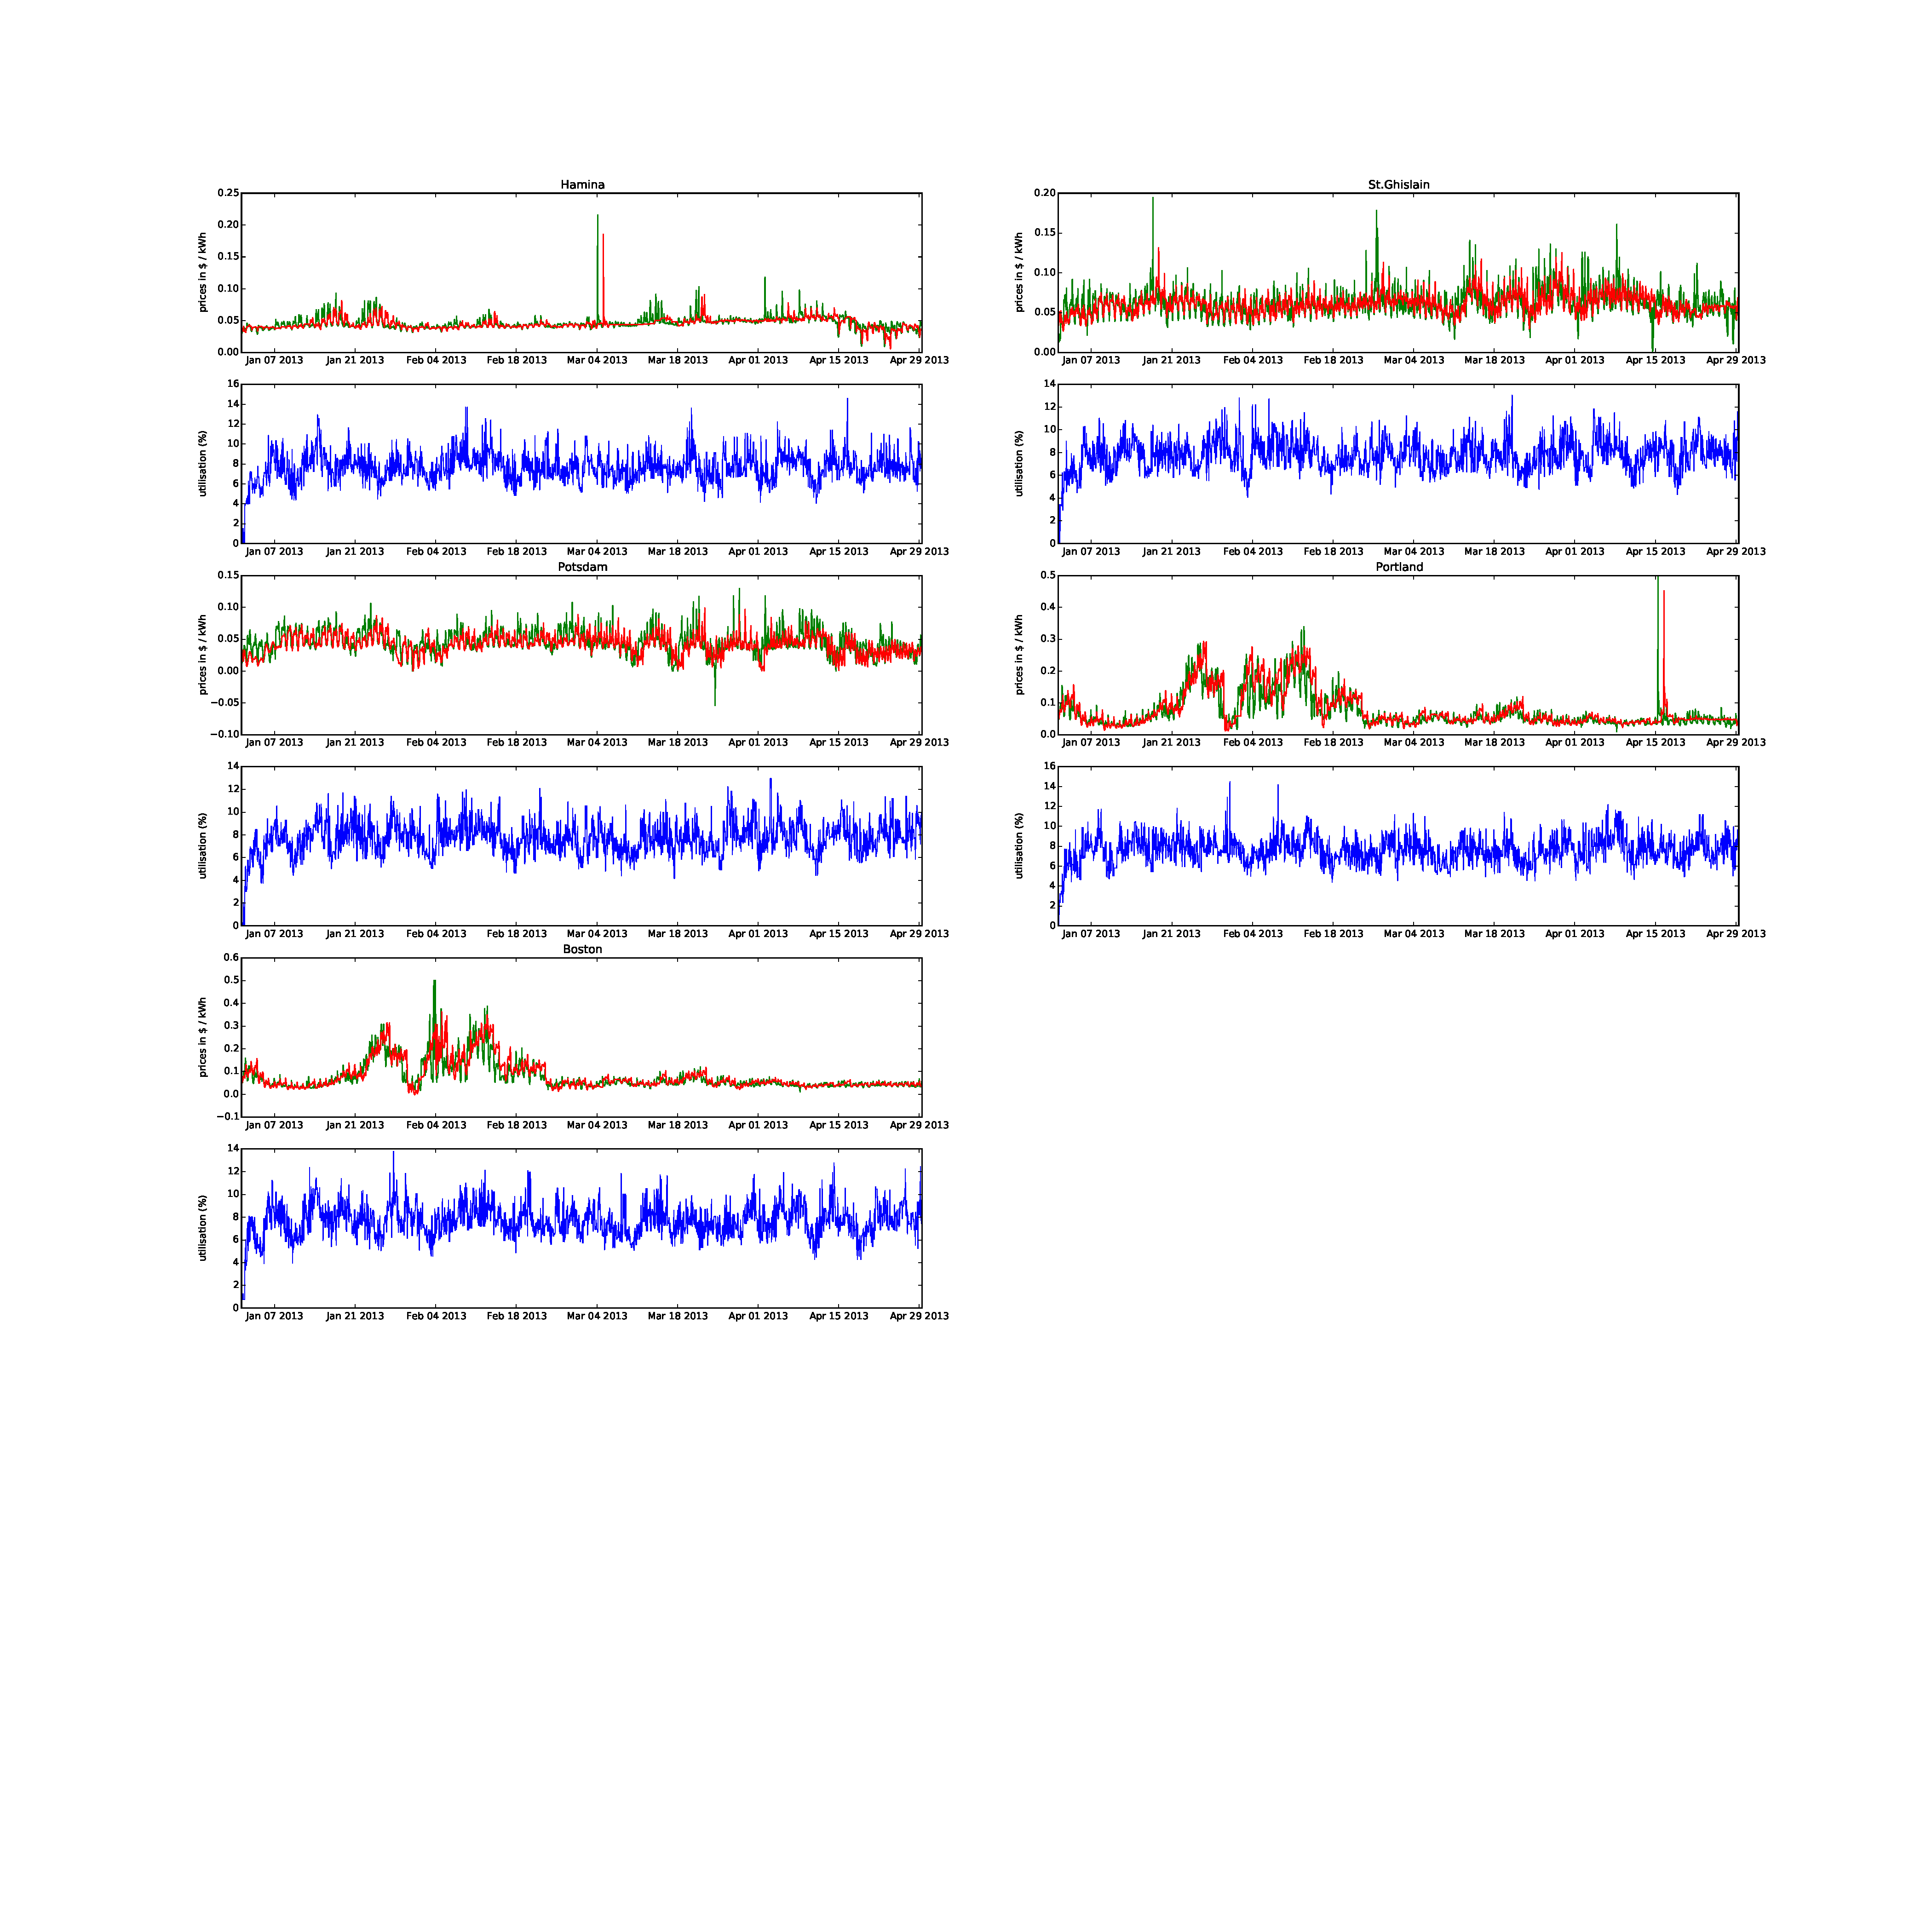
\includegraphics[width=1.60\textwidth]{figures/appendix_simulation_results/DA_Spring_scenario_1.pdf}
	\vspace*{-2.8in}
	\caption{Energy prices, energy price forecasts and utilization levels per location for simulation ``DA Spring'' and scheduler BFD}
	\label{fig:app_DA_Spring_scenario_1}
\end{figure}

\begin{figure}[htbp]
	\centering
	\vspace*{-0.6in}
	\hspace*{-1.9in}
		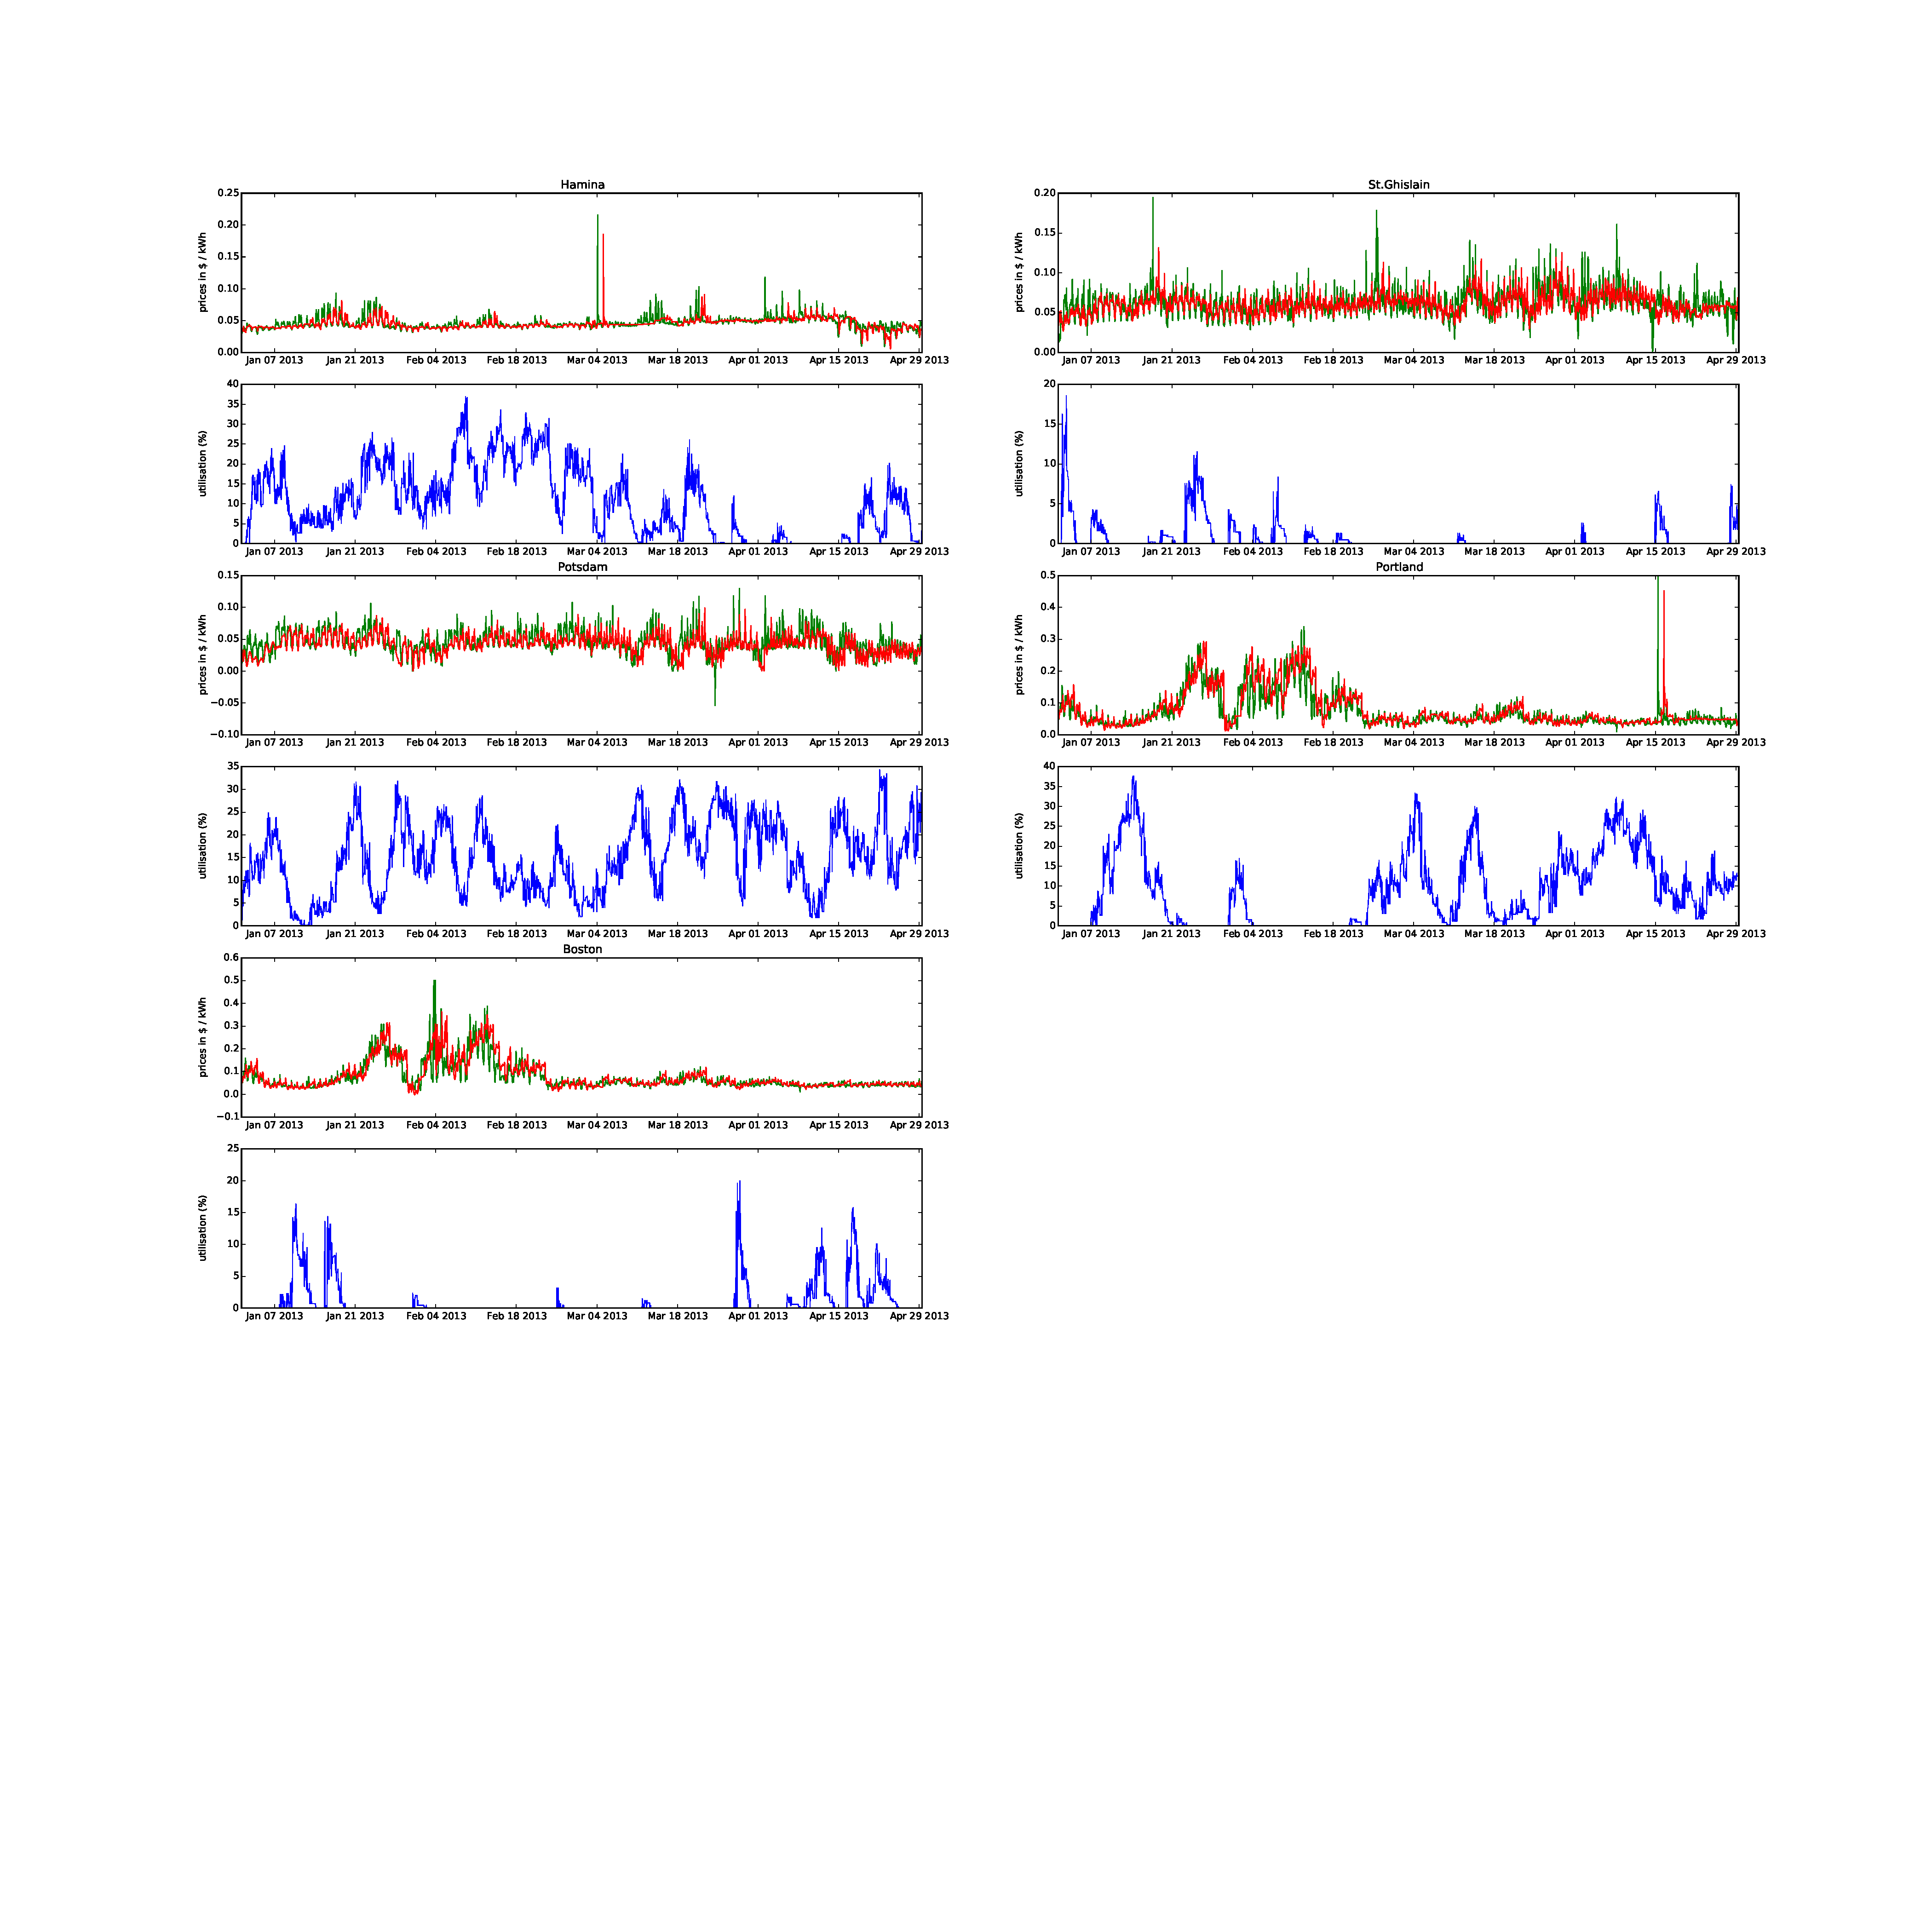
\includegraphics[width=1.60\textwidth]{figures/appendix_simulation_results/DA_Spring_scenario_2.pdf}
	\vspace*{-2.8in}
	\caption{Energy prices, energy price forecasts and utilization levels per location for simulation ``DA Spring'' and scheduler BCF}
	\label{fig:app_DA_Spring_scenario_2}
\end{figure}

\begin{figure}[htbp]
	\centering
	\vspace*{-0.6in}
	\hspace*{-1.4in}
		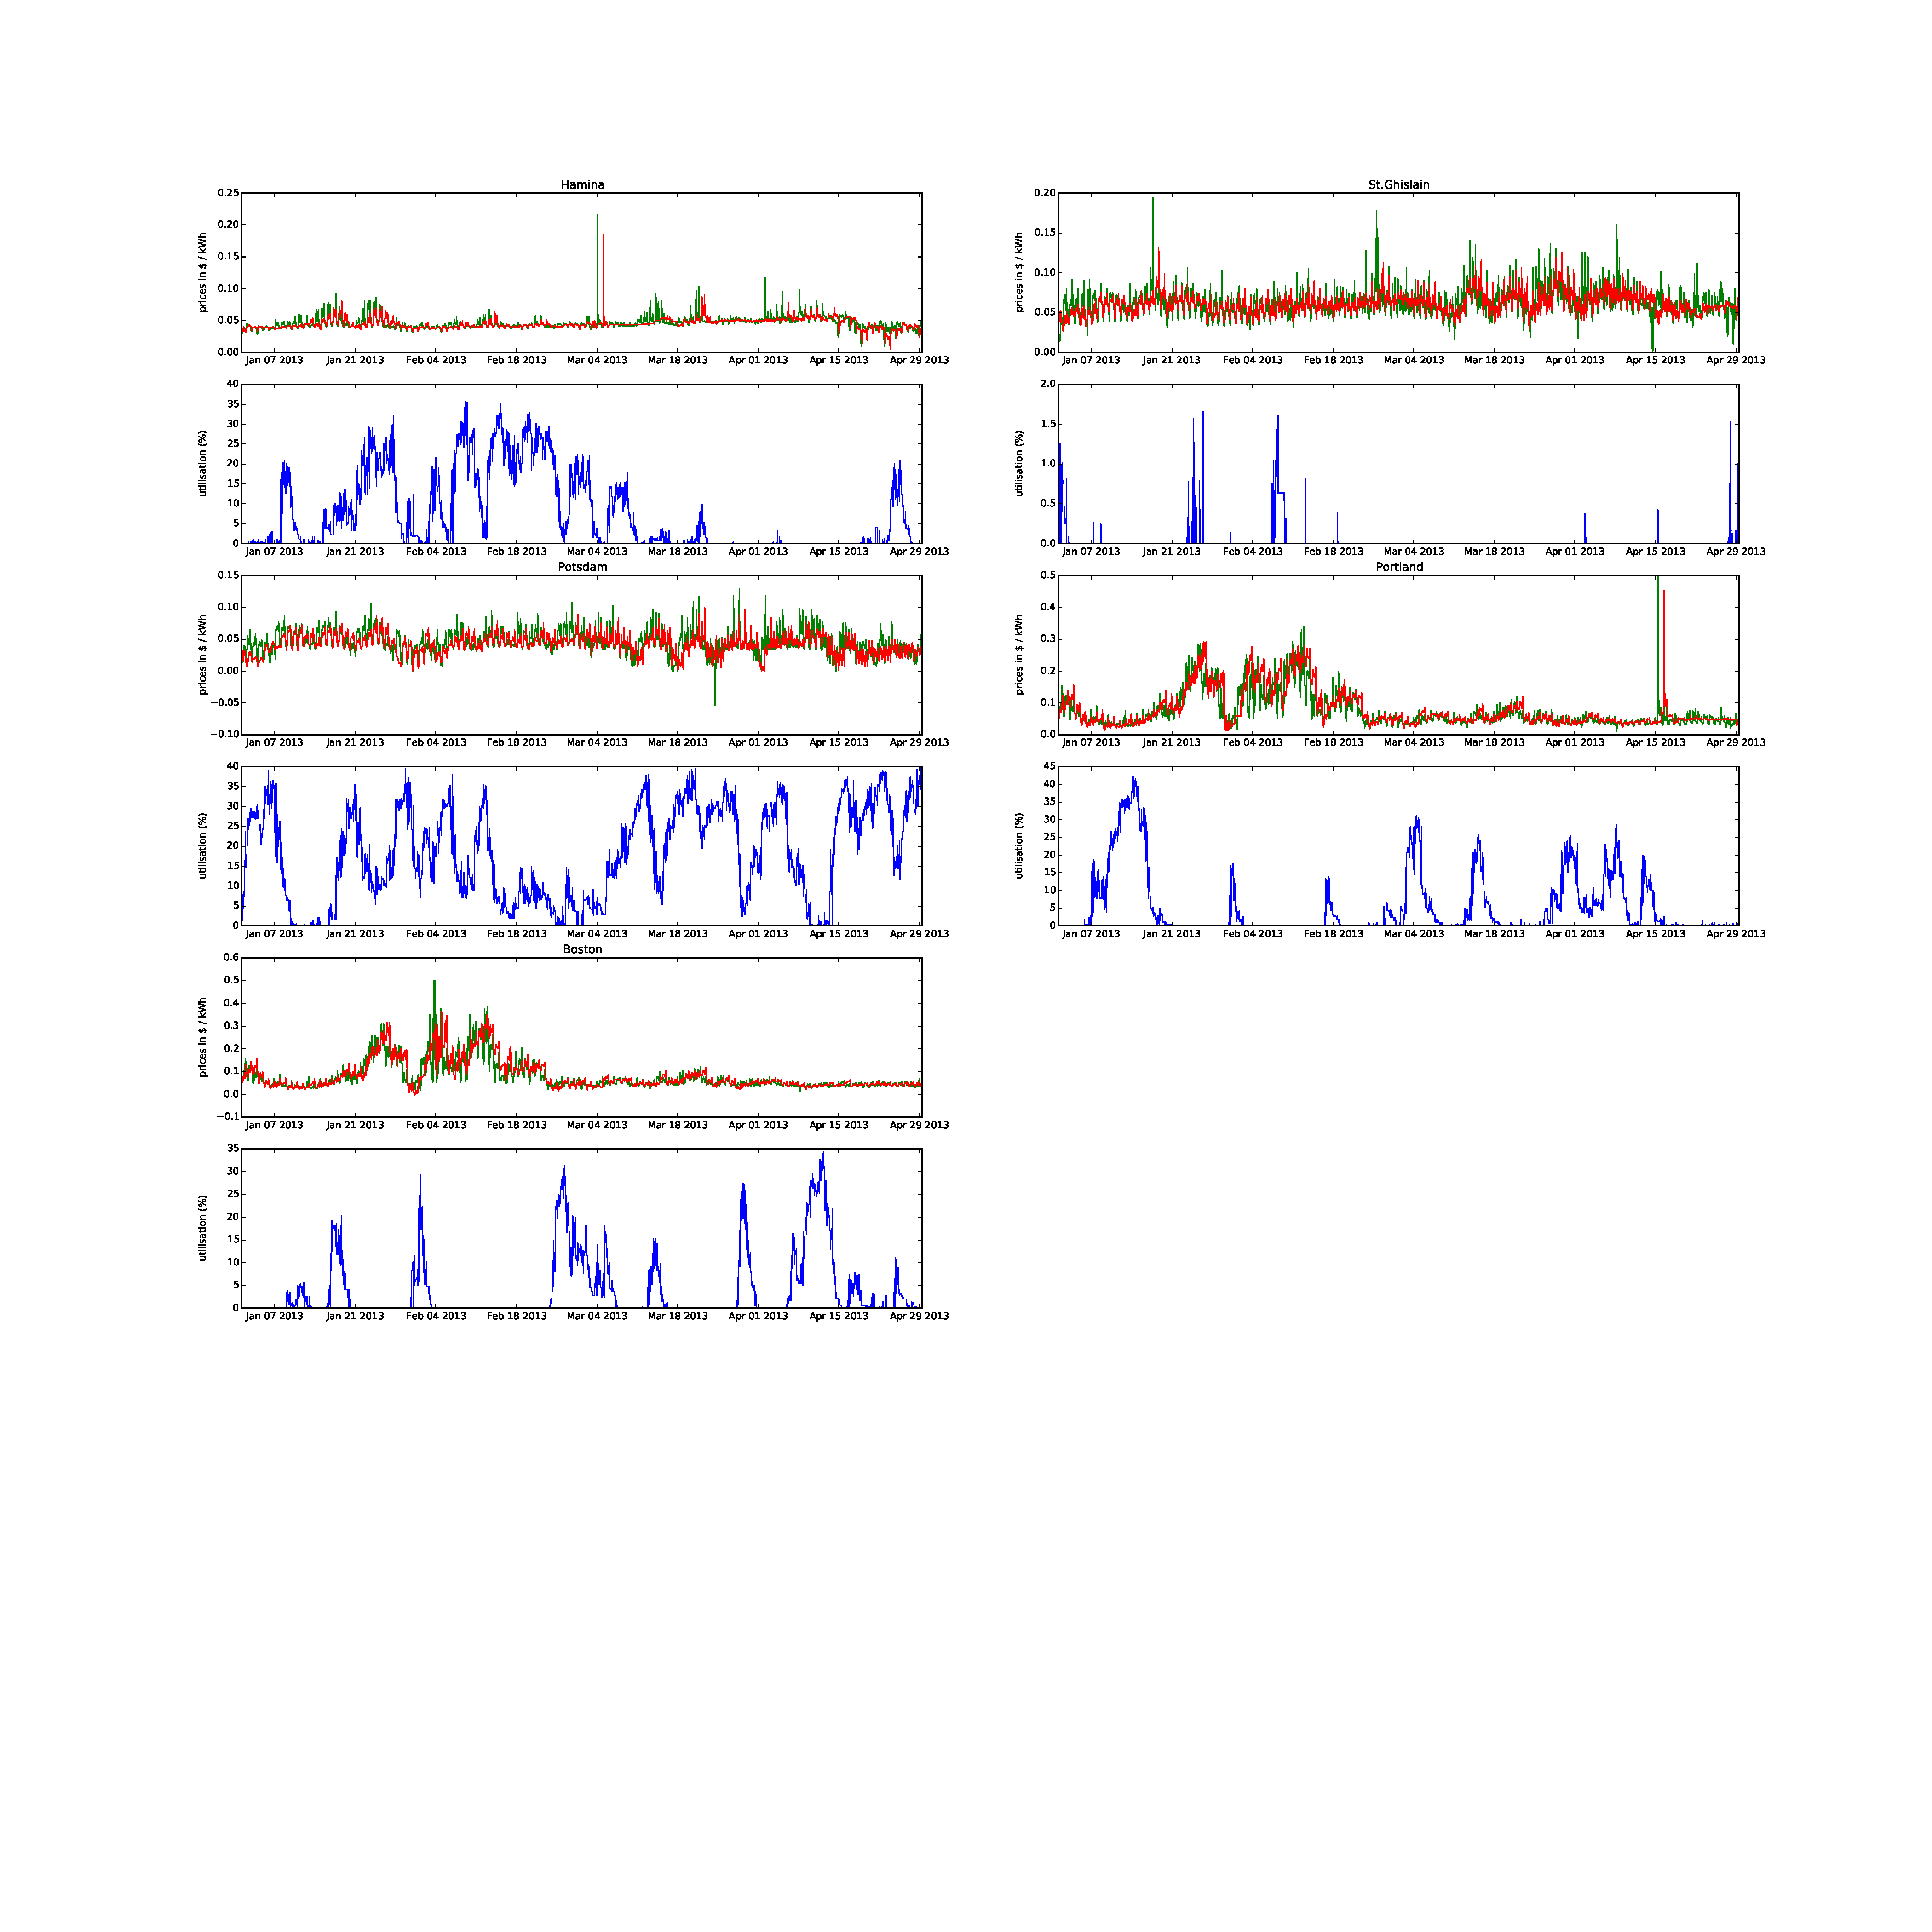
\includegraphics[width=1.60\textwidth]{figures/appendix_simulation_results/DA_Spring_scenario_3.pdf}
	\vspace*{-2.8in}
	\caption{Energy prices, energy price forecasts and utilization levels per location for simulation ``DA Spring'' and scheduler BCF\_F}
	\label{fig:app_DA_Spring_scenario_3}
\end{figure}

\begin{figure}[htbp]
	\centering
	\vspace*{-0.6in}
	\hspace*{-1.9in}
		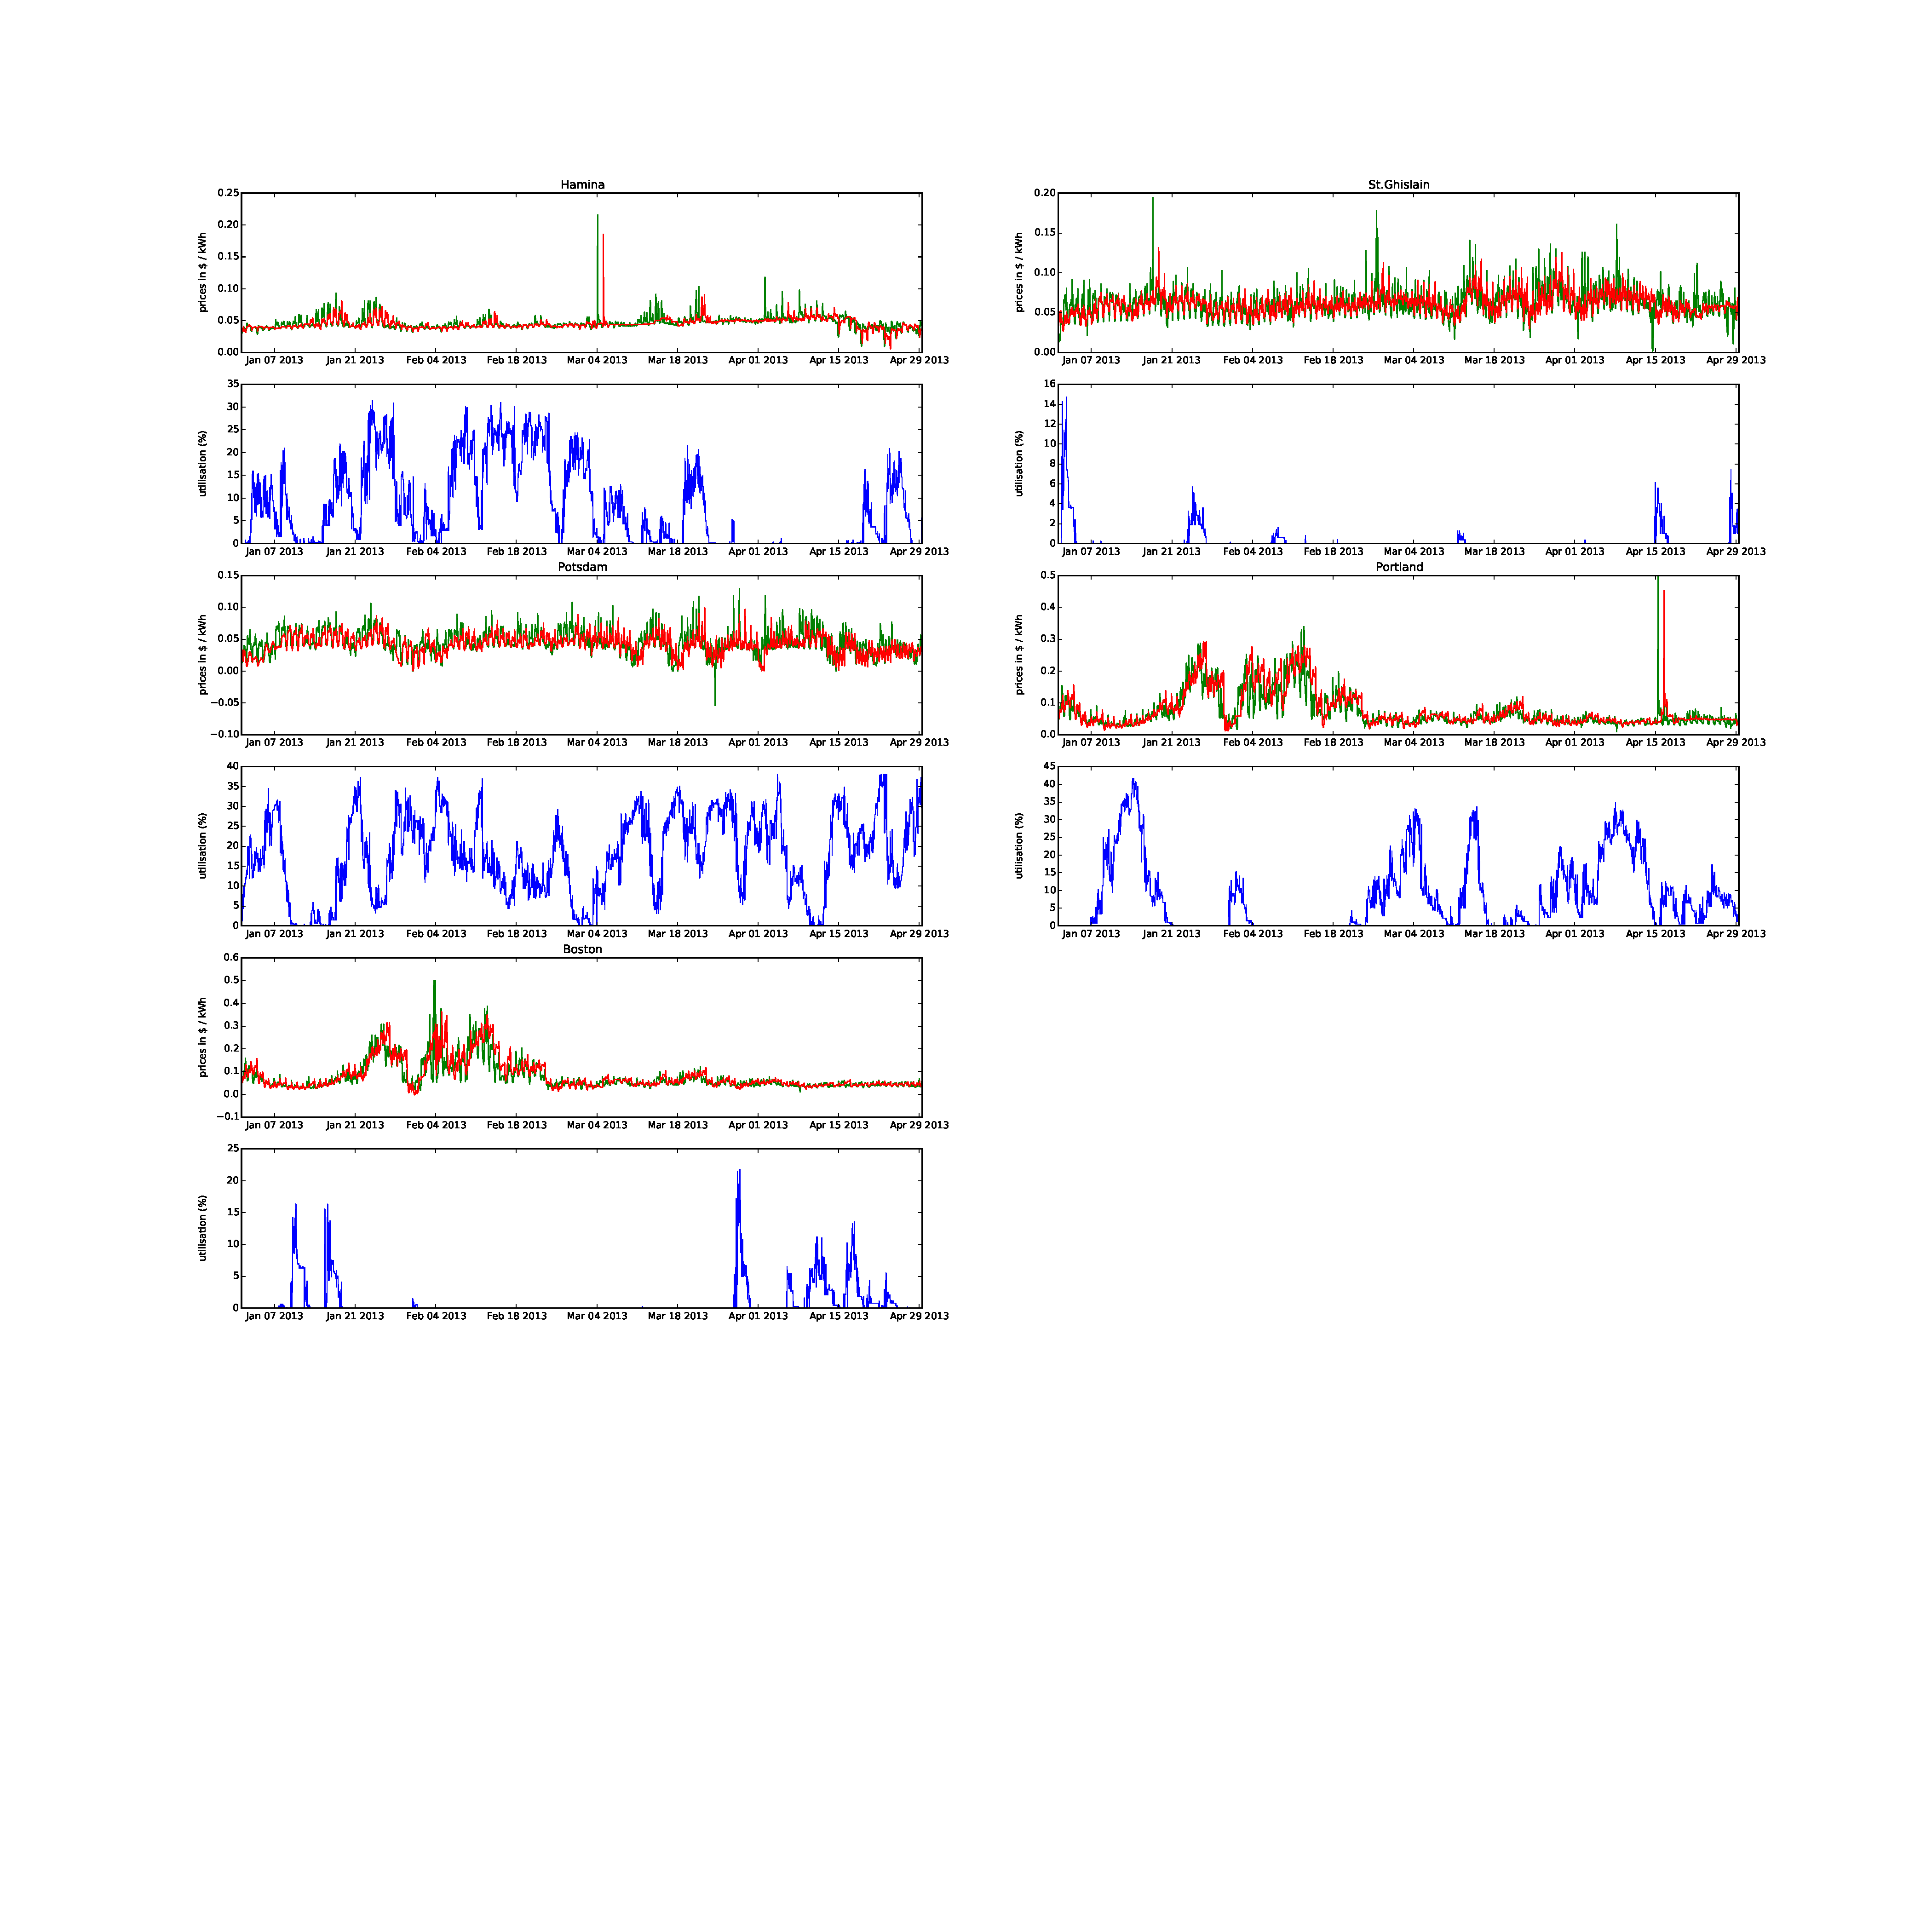
\includegraphics[width=1.60\textwidth]{figures/appendix_simulation_results/DA_Spring_scenario_4.pdf}
	\vspace*{-2.8in}
	\caption{Energy prices, energy price forecasts and utilization levels per location for simulation ``DA Spring'' and scheduler BCF\_IF}
	\label{fig:app_DA_Spring_scenario_4}
\end{figure}

\begin{figure}[htbp]
	\centering
	\vspace*{-0.6in}
	\hspace*{-1.4in}
		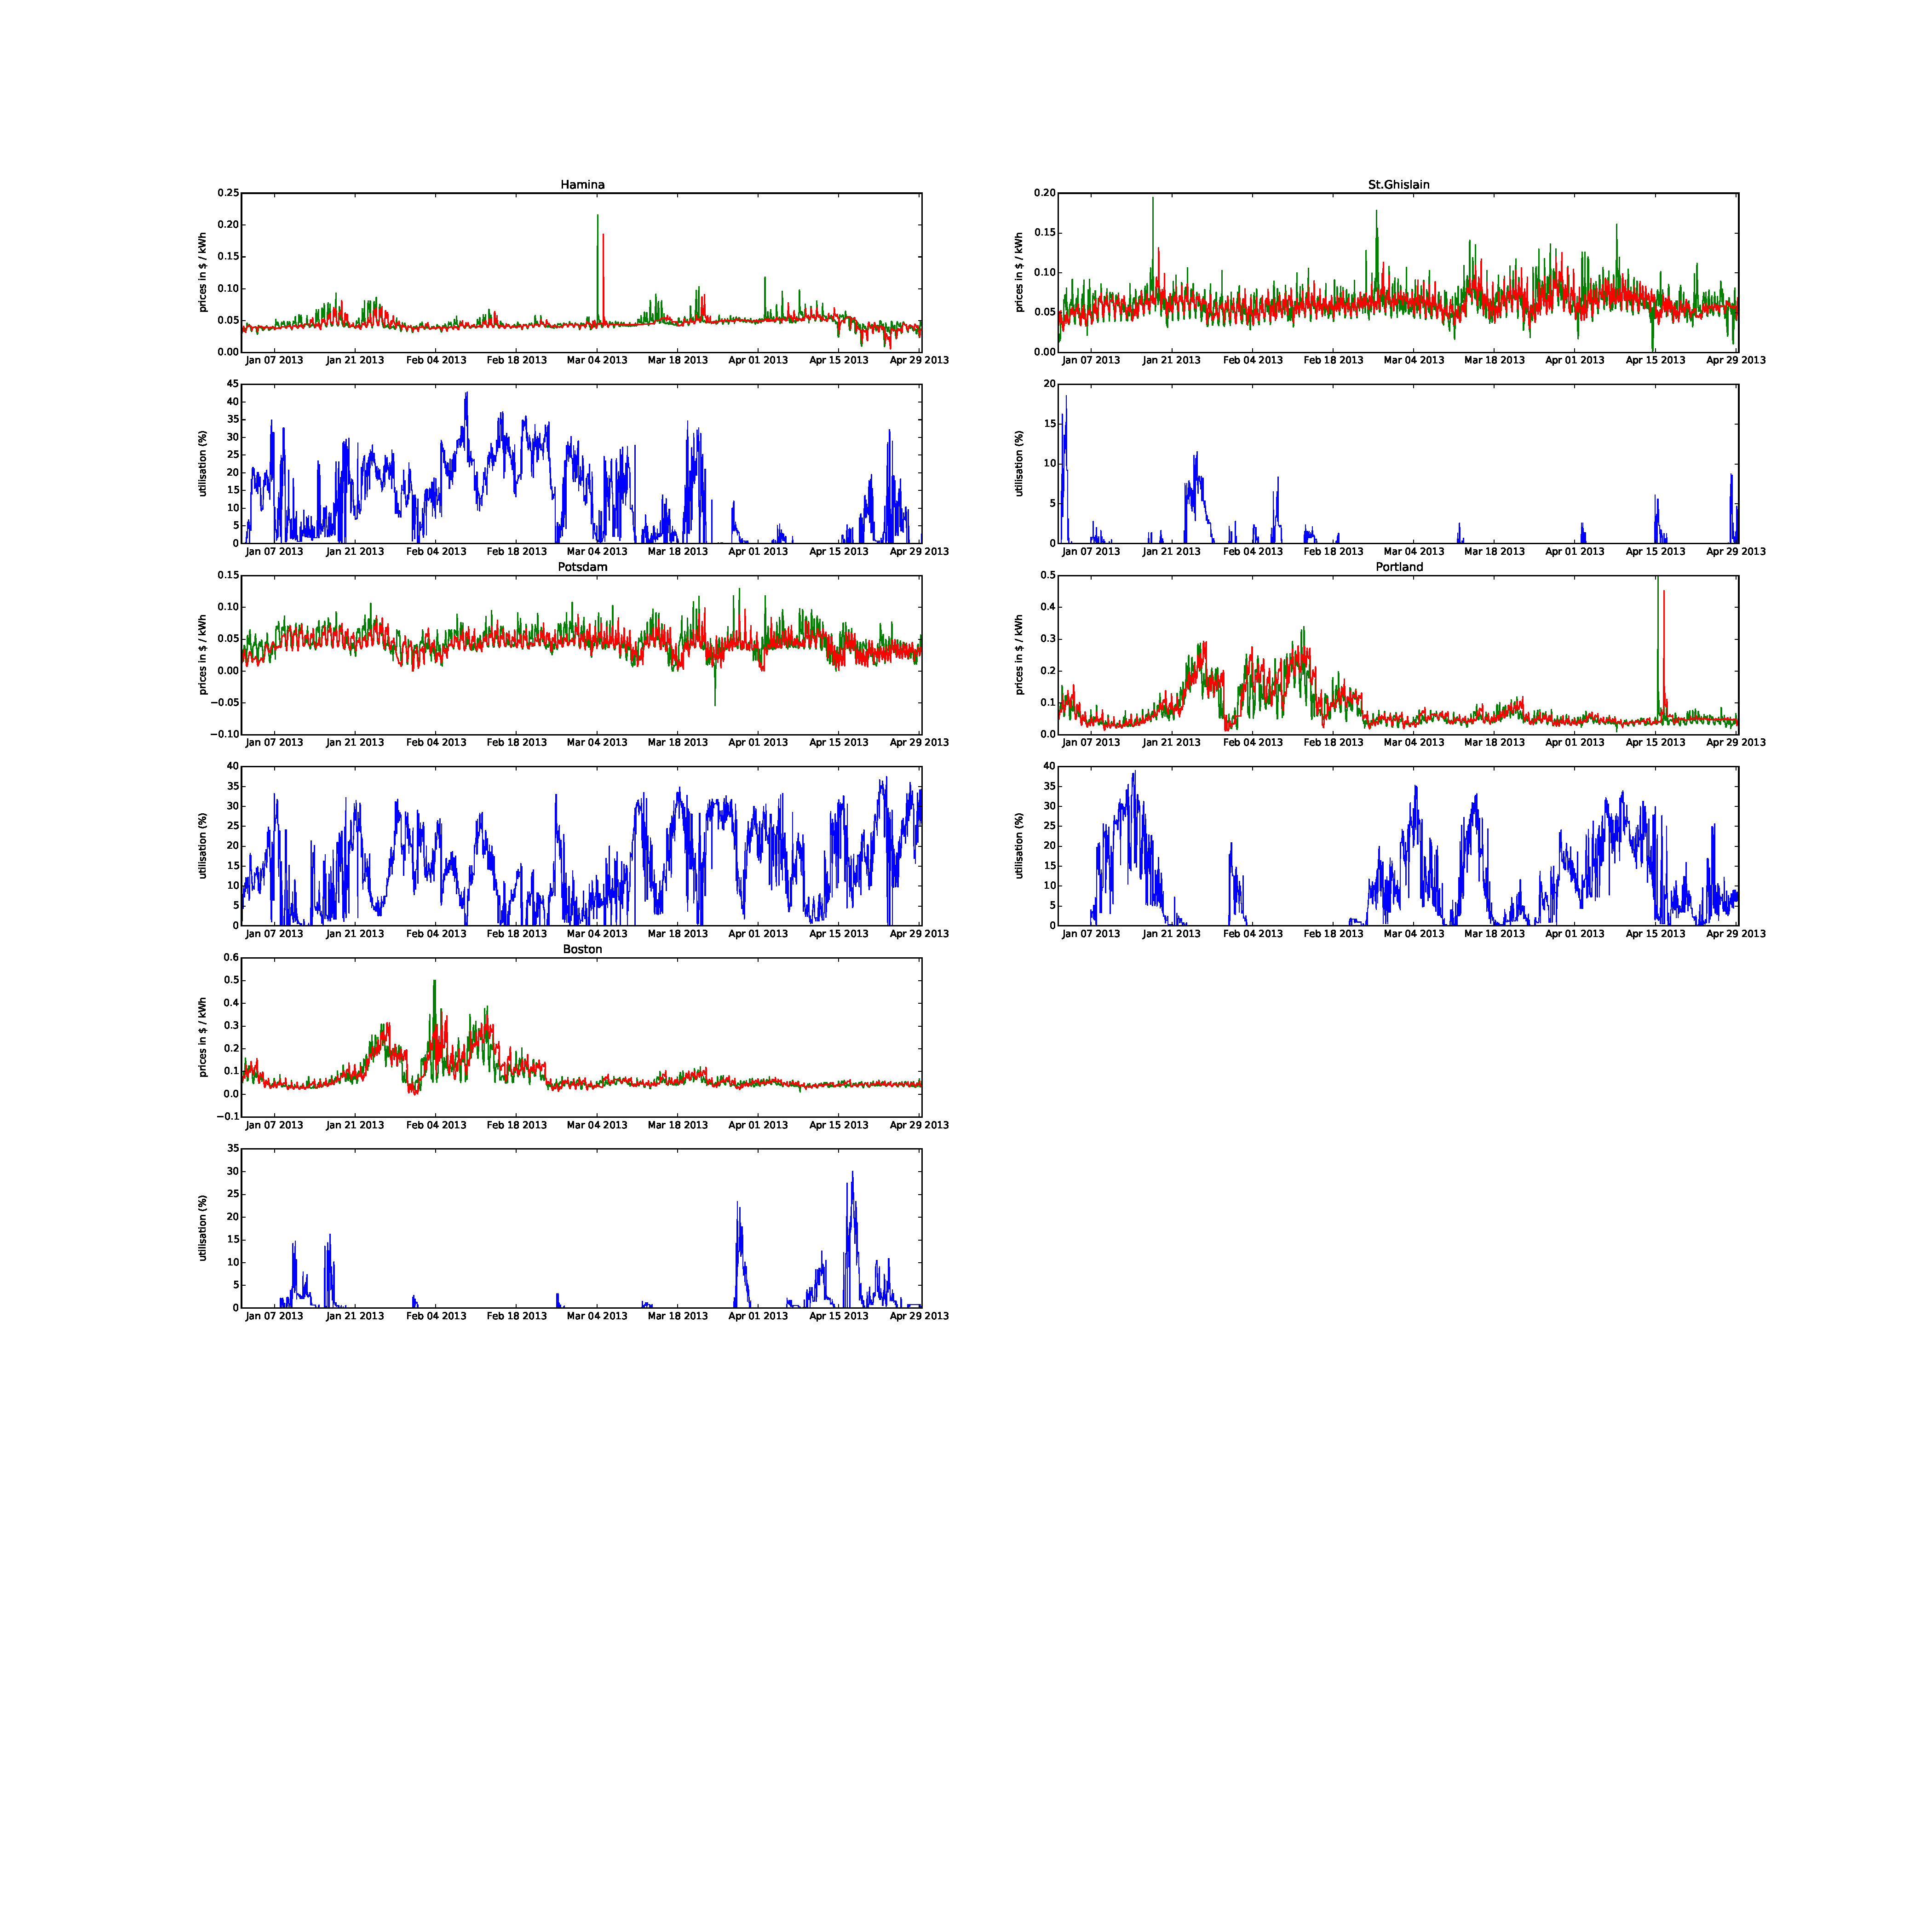
\includegraphics[width=1.60\textwidth]{figures/appendix_simulation_results/DA_Spring_scenario_5.pdf}
	\vspace*{-2.8in}
	\caption{Energy prices, energy price forecasts and utilization levels per location for simulation ``DA Spring'' and scheduler BCU\_M}
	\label{fig:app_DA_Spring_scenario_5}
\end{figure}

\begin{figure}[htbp]
	\centering
	\vspace*{-0.6in}
	\hspace*{-1.9in}
		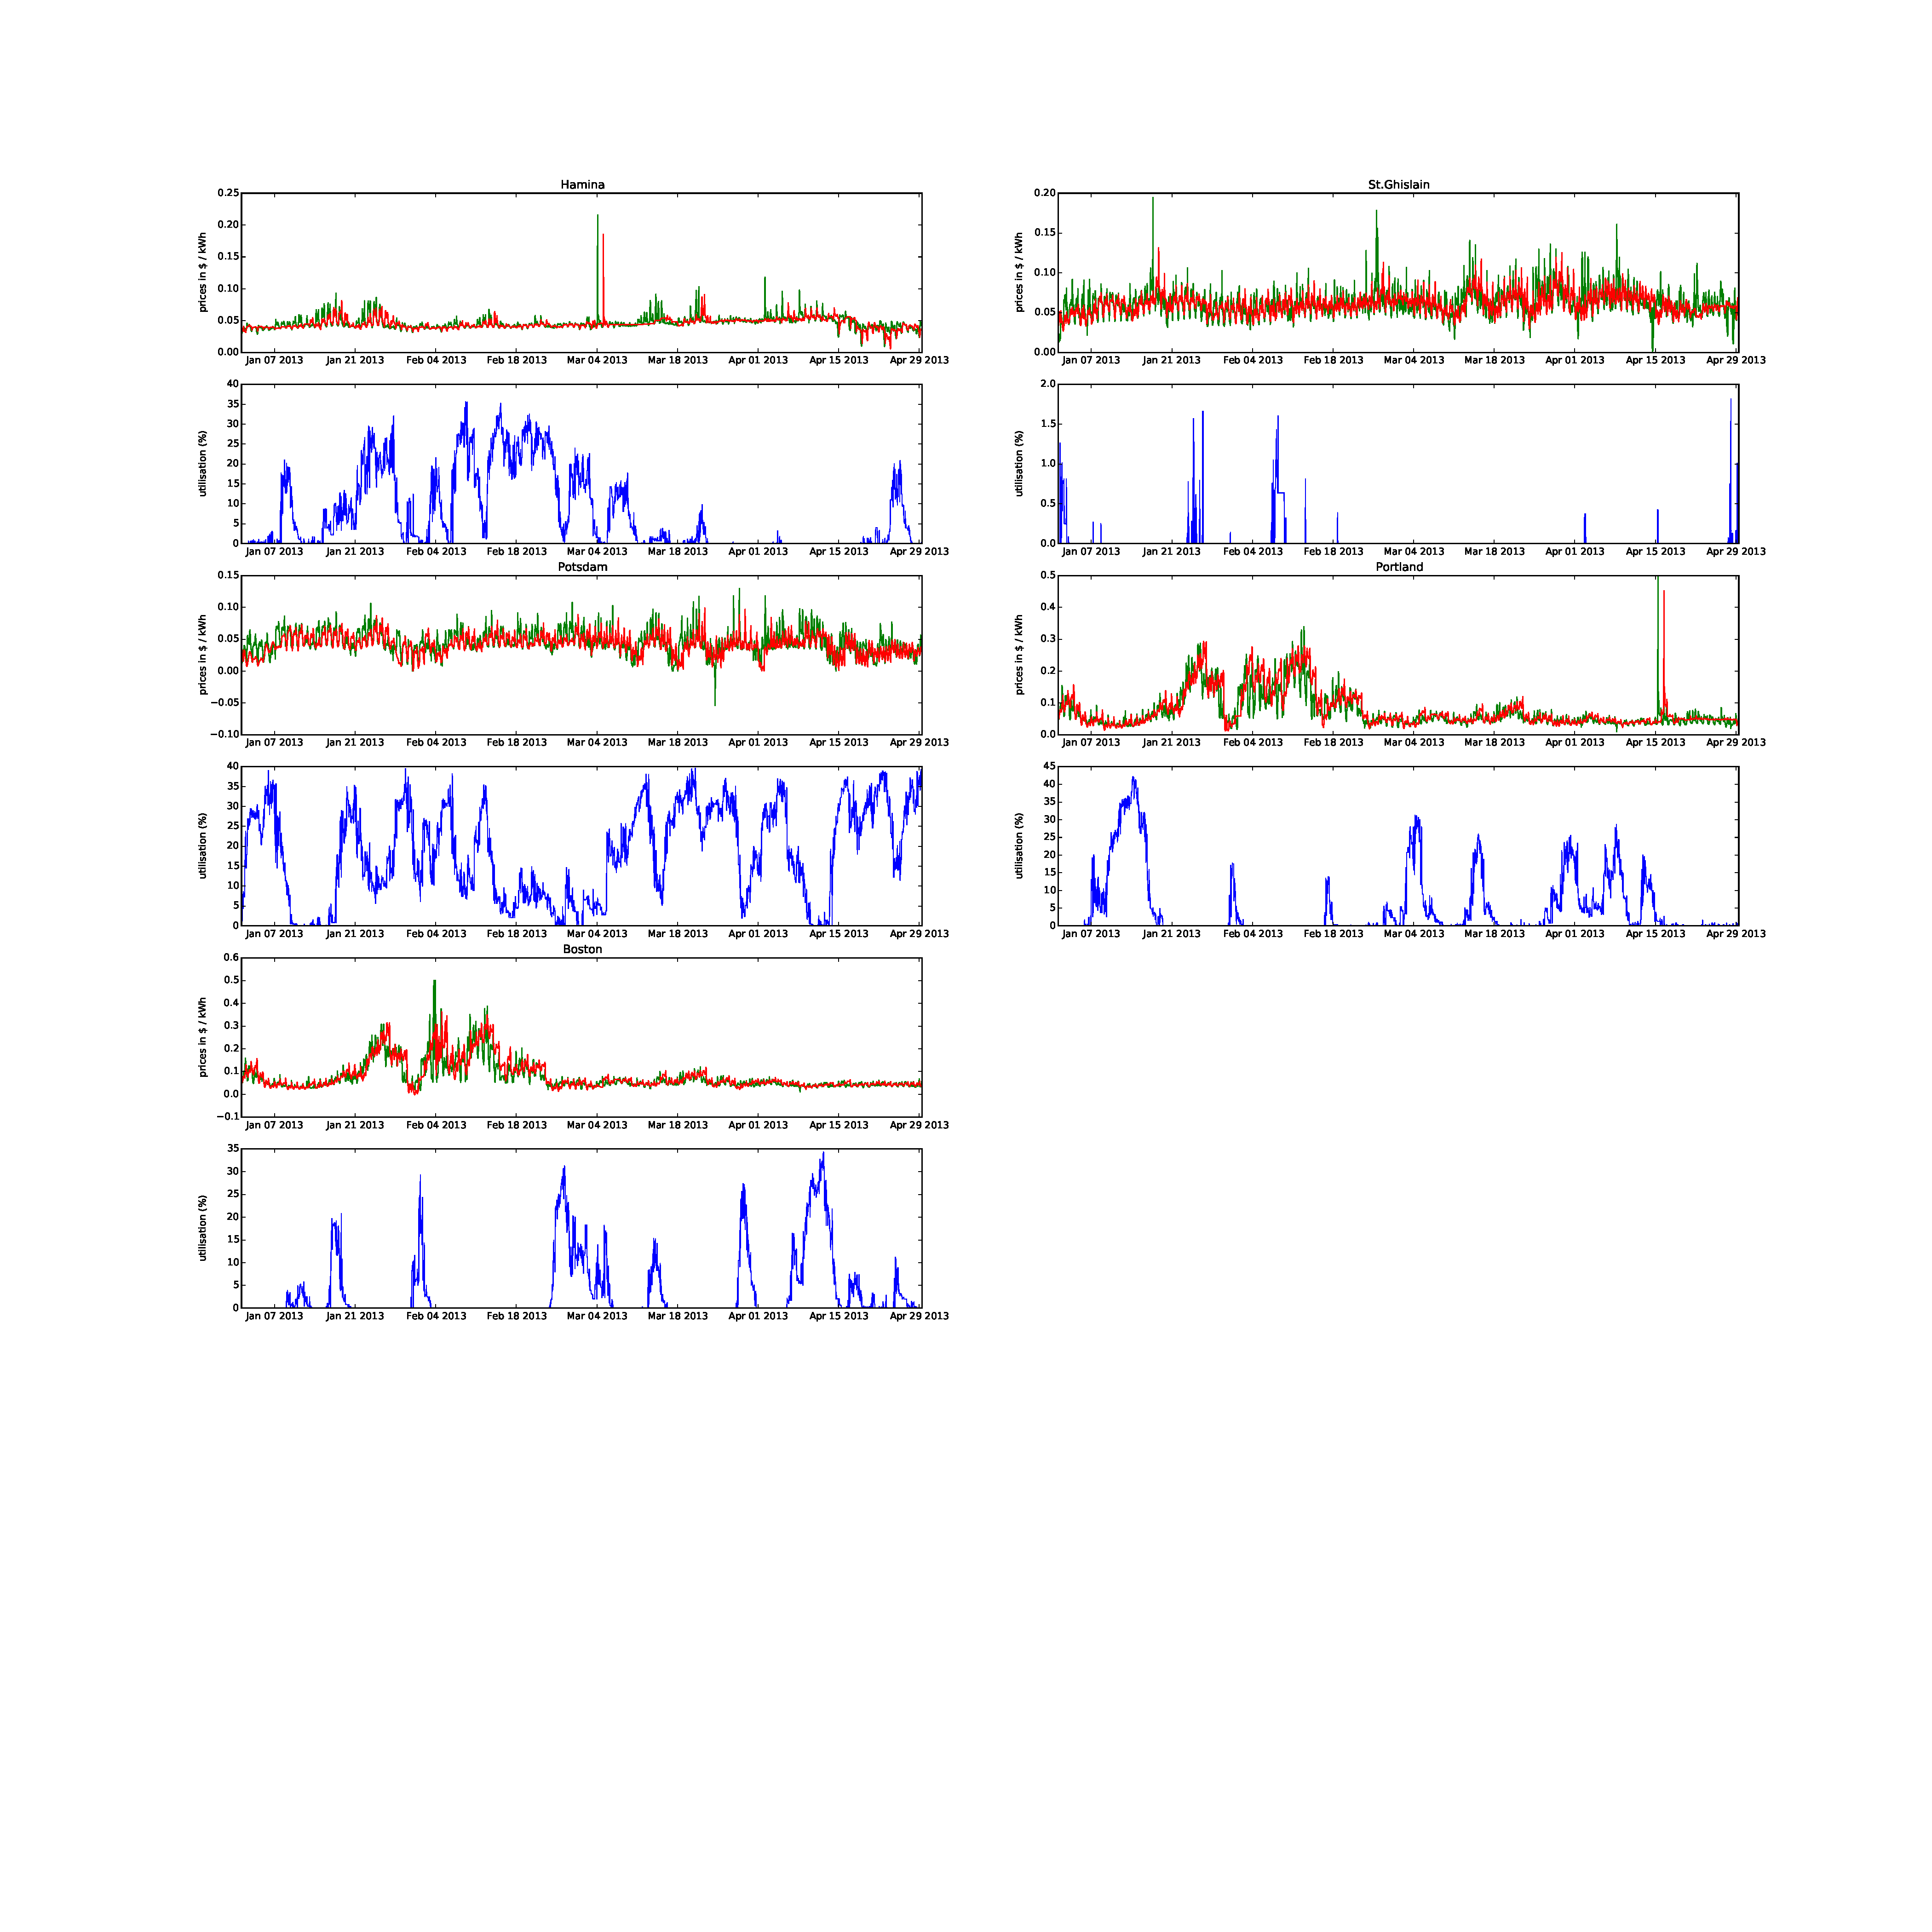
\includegraphics[width=1.60\textwidth]{figures/appendix_simulation_results/DA_Spring_scenario_6.pdf}
	\vspace*{-2.8in}
	\caption{Energy prices, energy price forecasts and utilization levels per location for simulation ``DA Spring'' and scheduler BCU\_MF}
	\label{fig:app_DA_Spring_scenario_6}
\end{figure}

\begin{figure}[htbp]
	\centering
	\vspace*{-0.6in}
	\hspace*{-1.4in}
		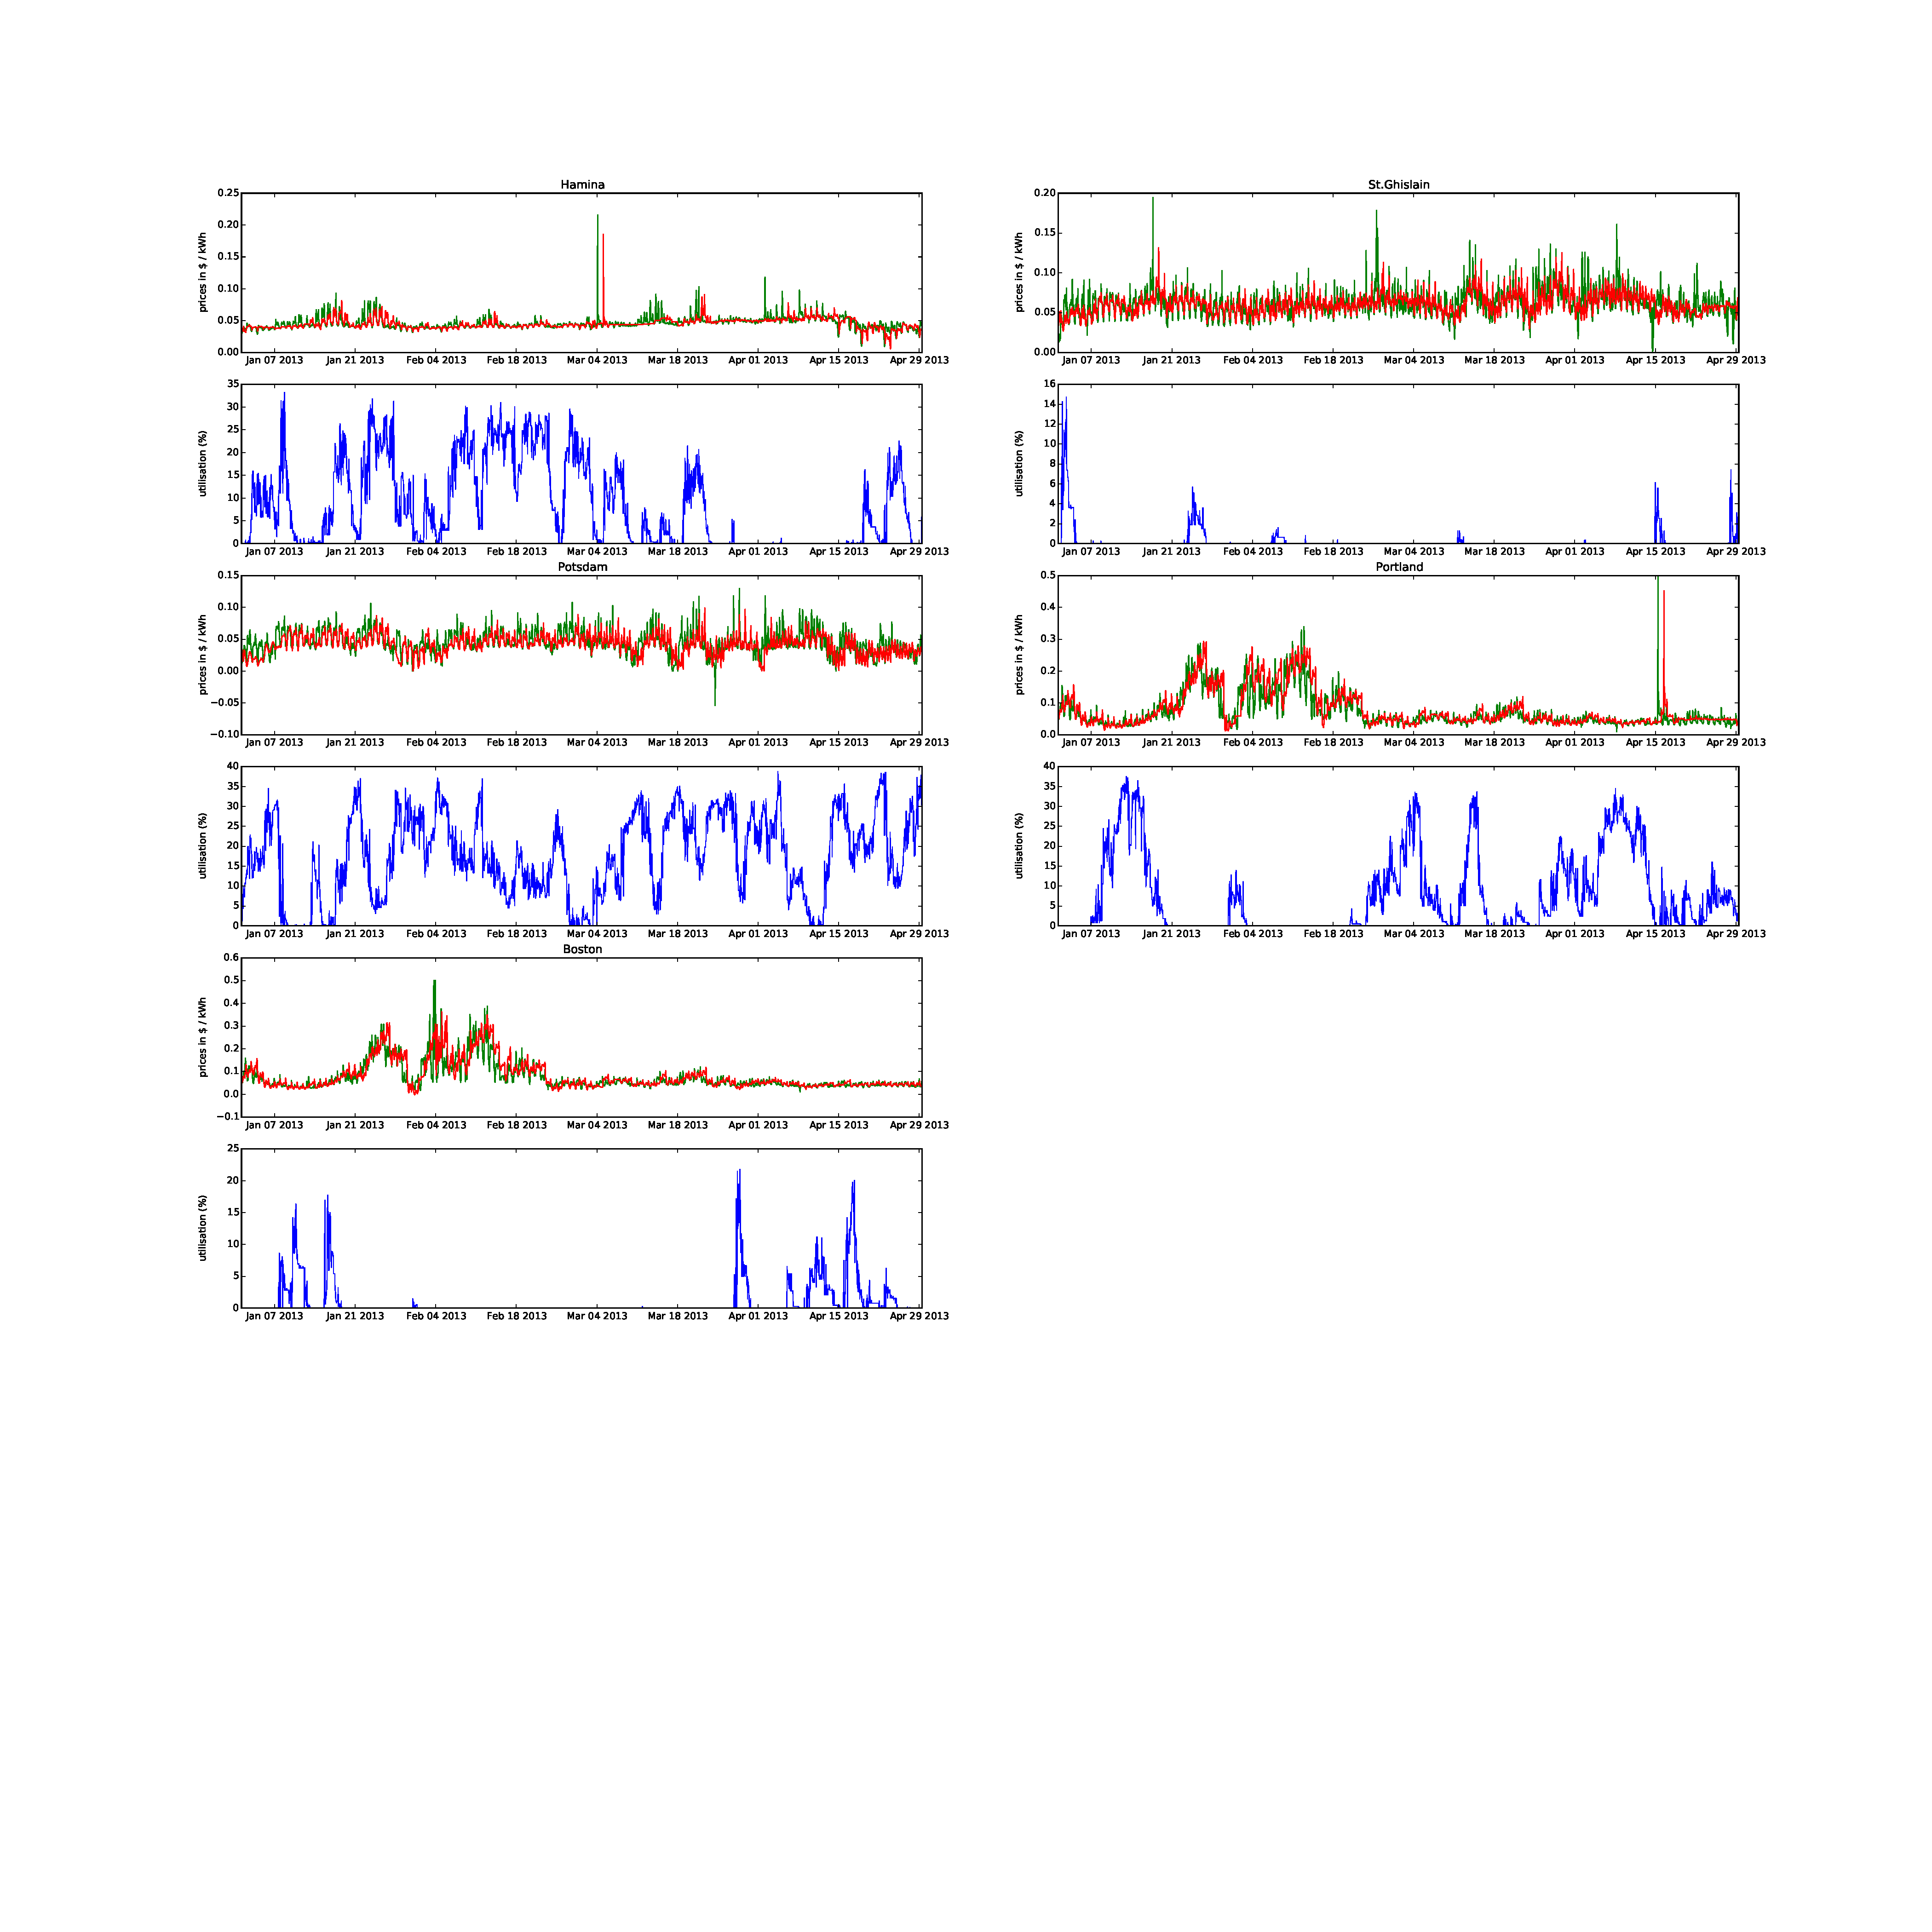
\includegraphics[width=1.60\textwidth]{figures/appendix_simulation_results/DA_Spring_scenario_7.pdf}
	\vspace*{-2.8in}
	\caption{Energy prices, energy price forecasts and utilization levels per location for simulation ``DA Spring'' and scheduler BCU\_MIF}
	\label{fig:app_DA_Spring_scenario_7}
\end{figure}


\FloatBarrier
\subsection{Simulation results for RT Summer}

\begin{figure}[htbp]
	\centering
	\vspace*{-0.6in}
	\hspace*{-1.4in}
		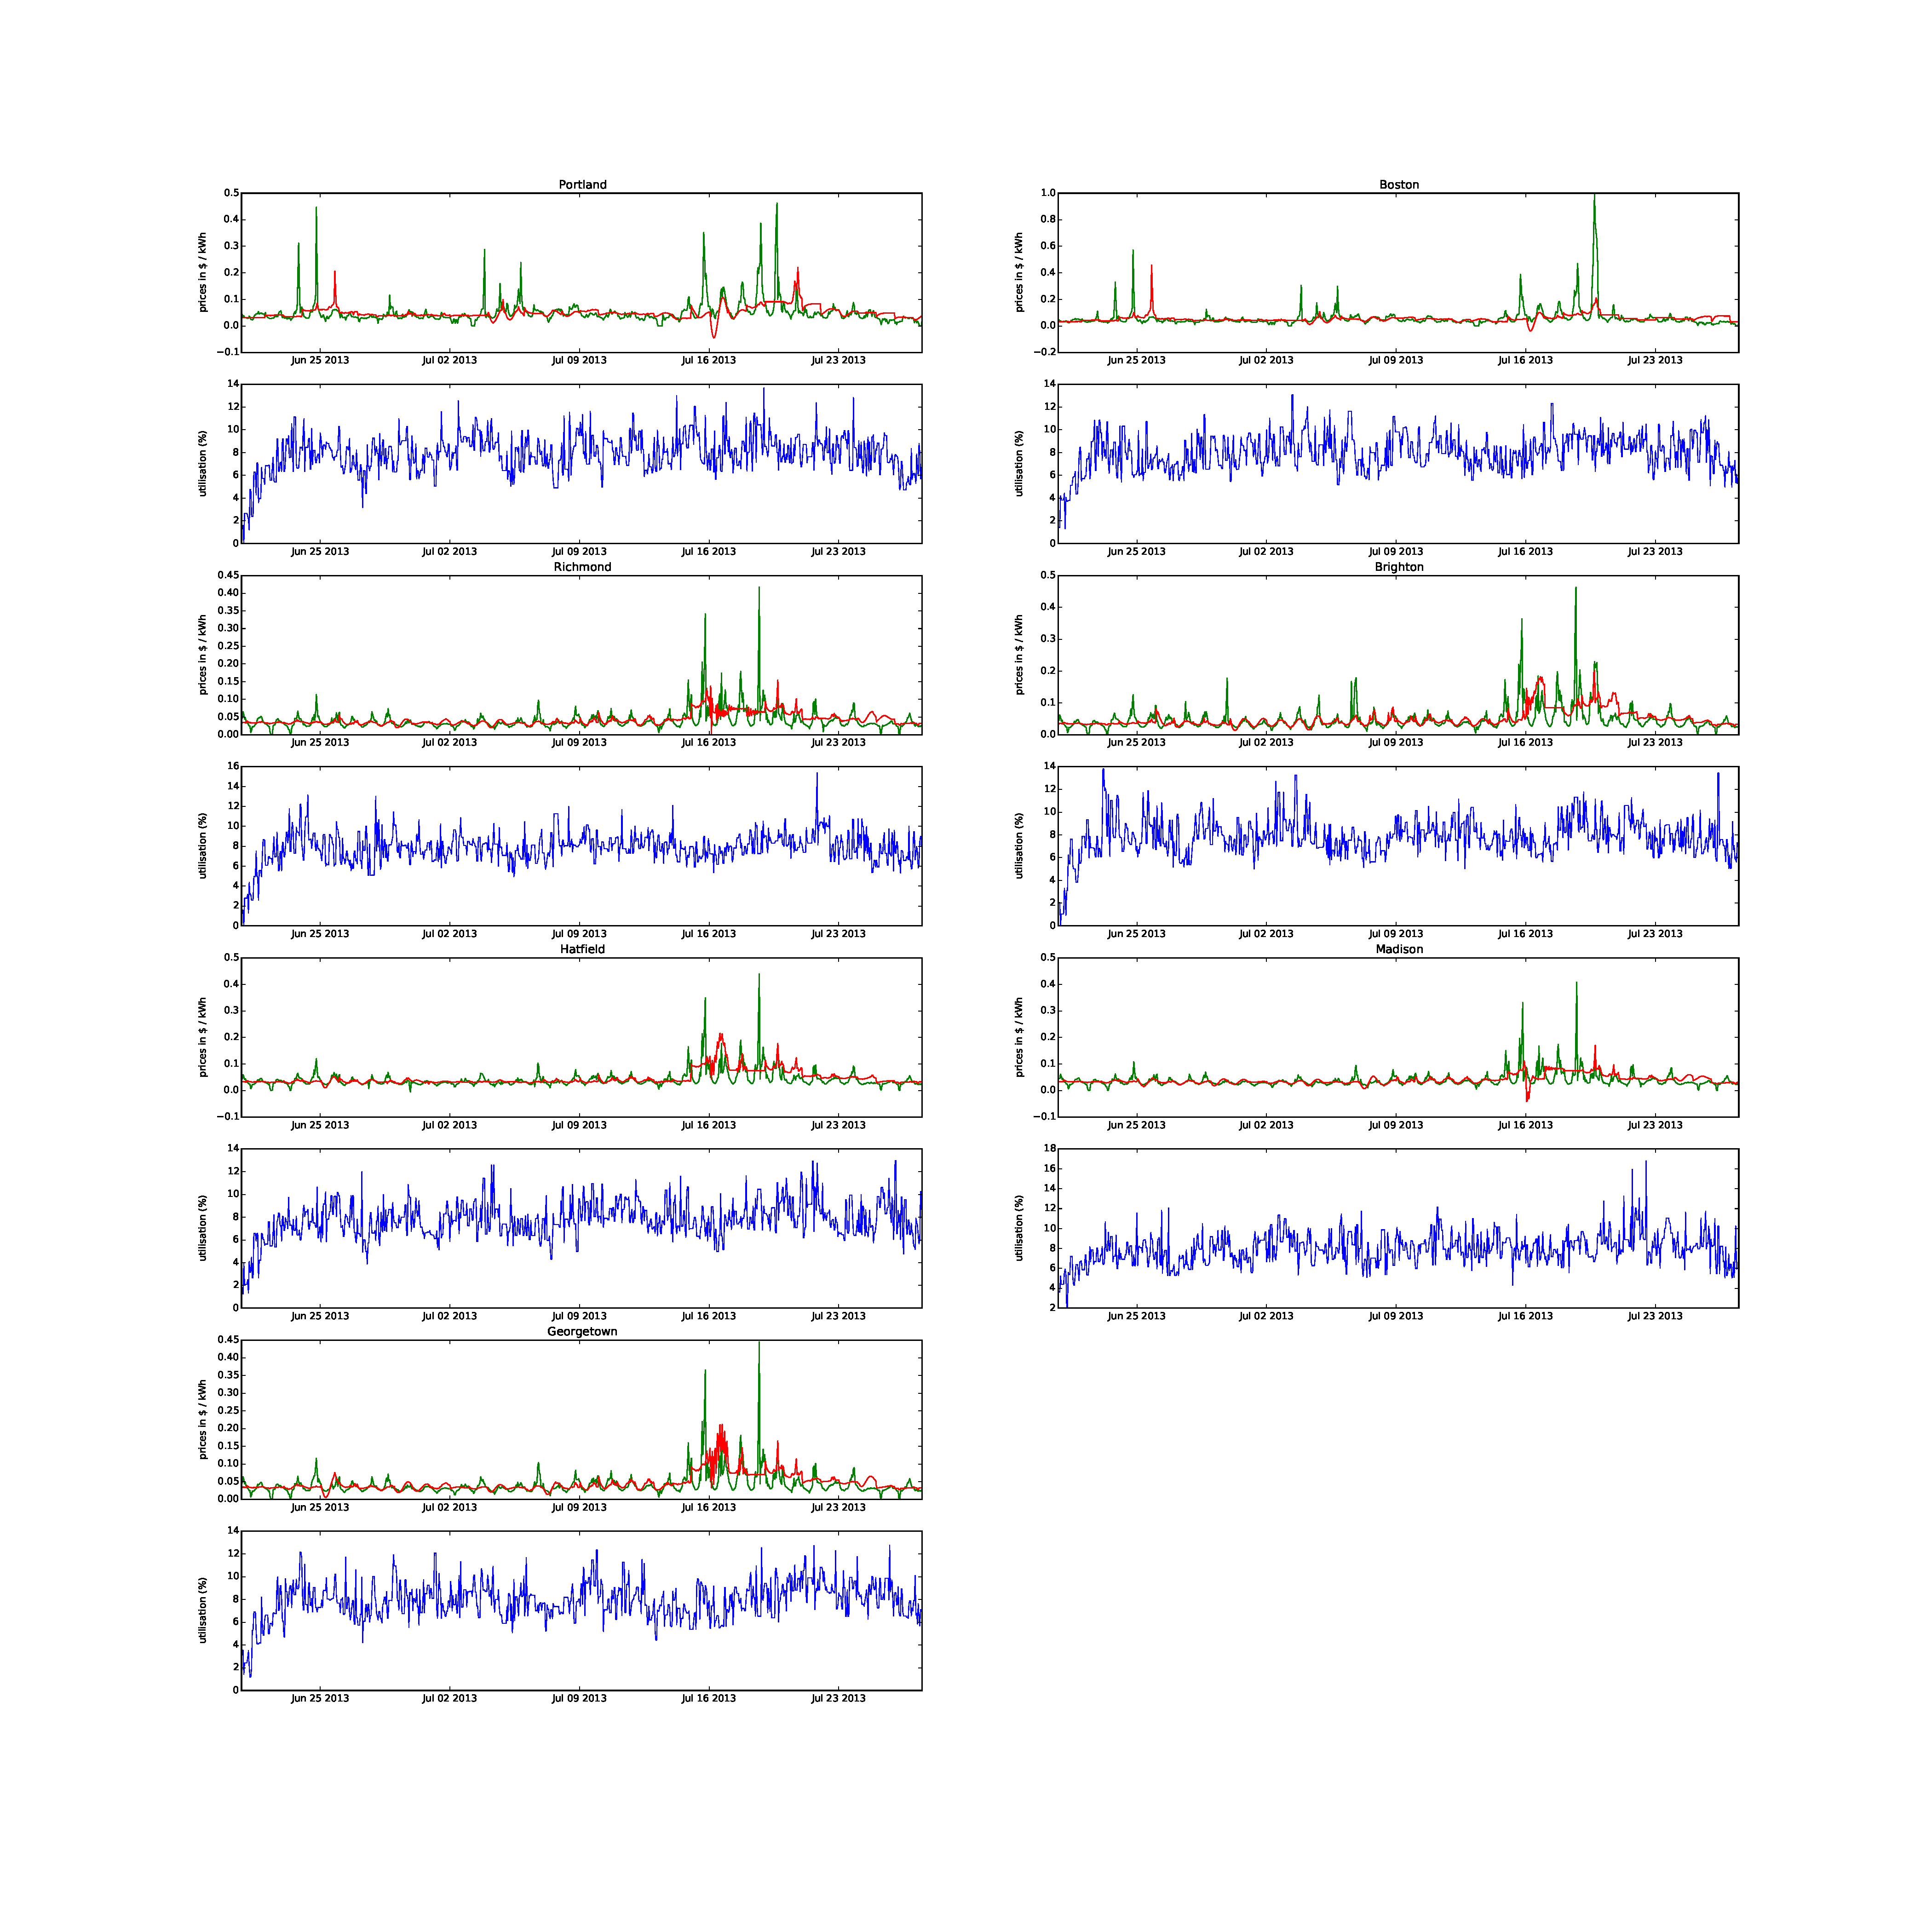
\includegraphics[width=1.60\textwidth]{figures/appendix_simulation_results/RT_Summer_scenario_1.pdf}
	\vspace*{-1.0in}
	\caption{Energy prices, energy price forecasts and utilization levels per location for simulation ``RT Summer'' and scheduler BFD}
	\label{fig:app_RT_Summer_scenario_1}
\end{figure}

\begin{figure}[htbp]
	\centering
	\vspace*{-0.6in}
	\hspace*{-1.9in}
		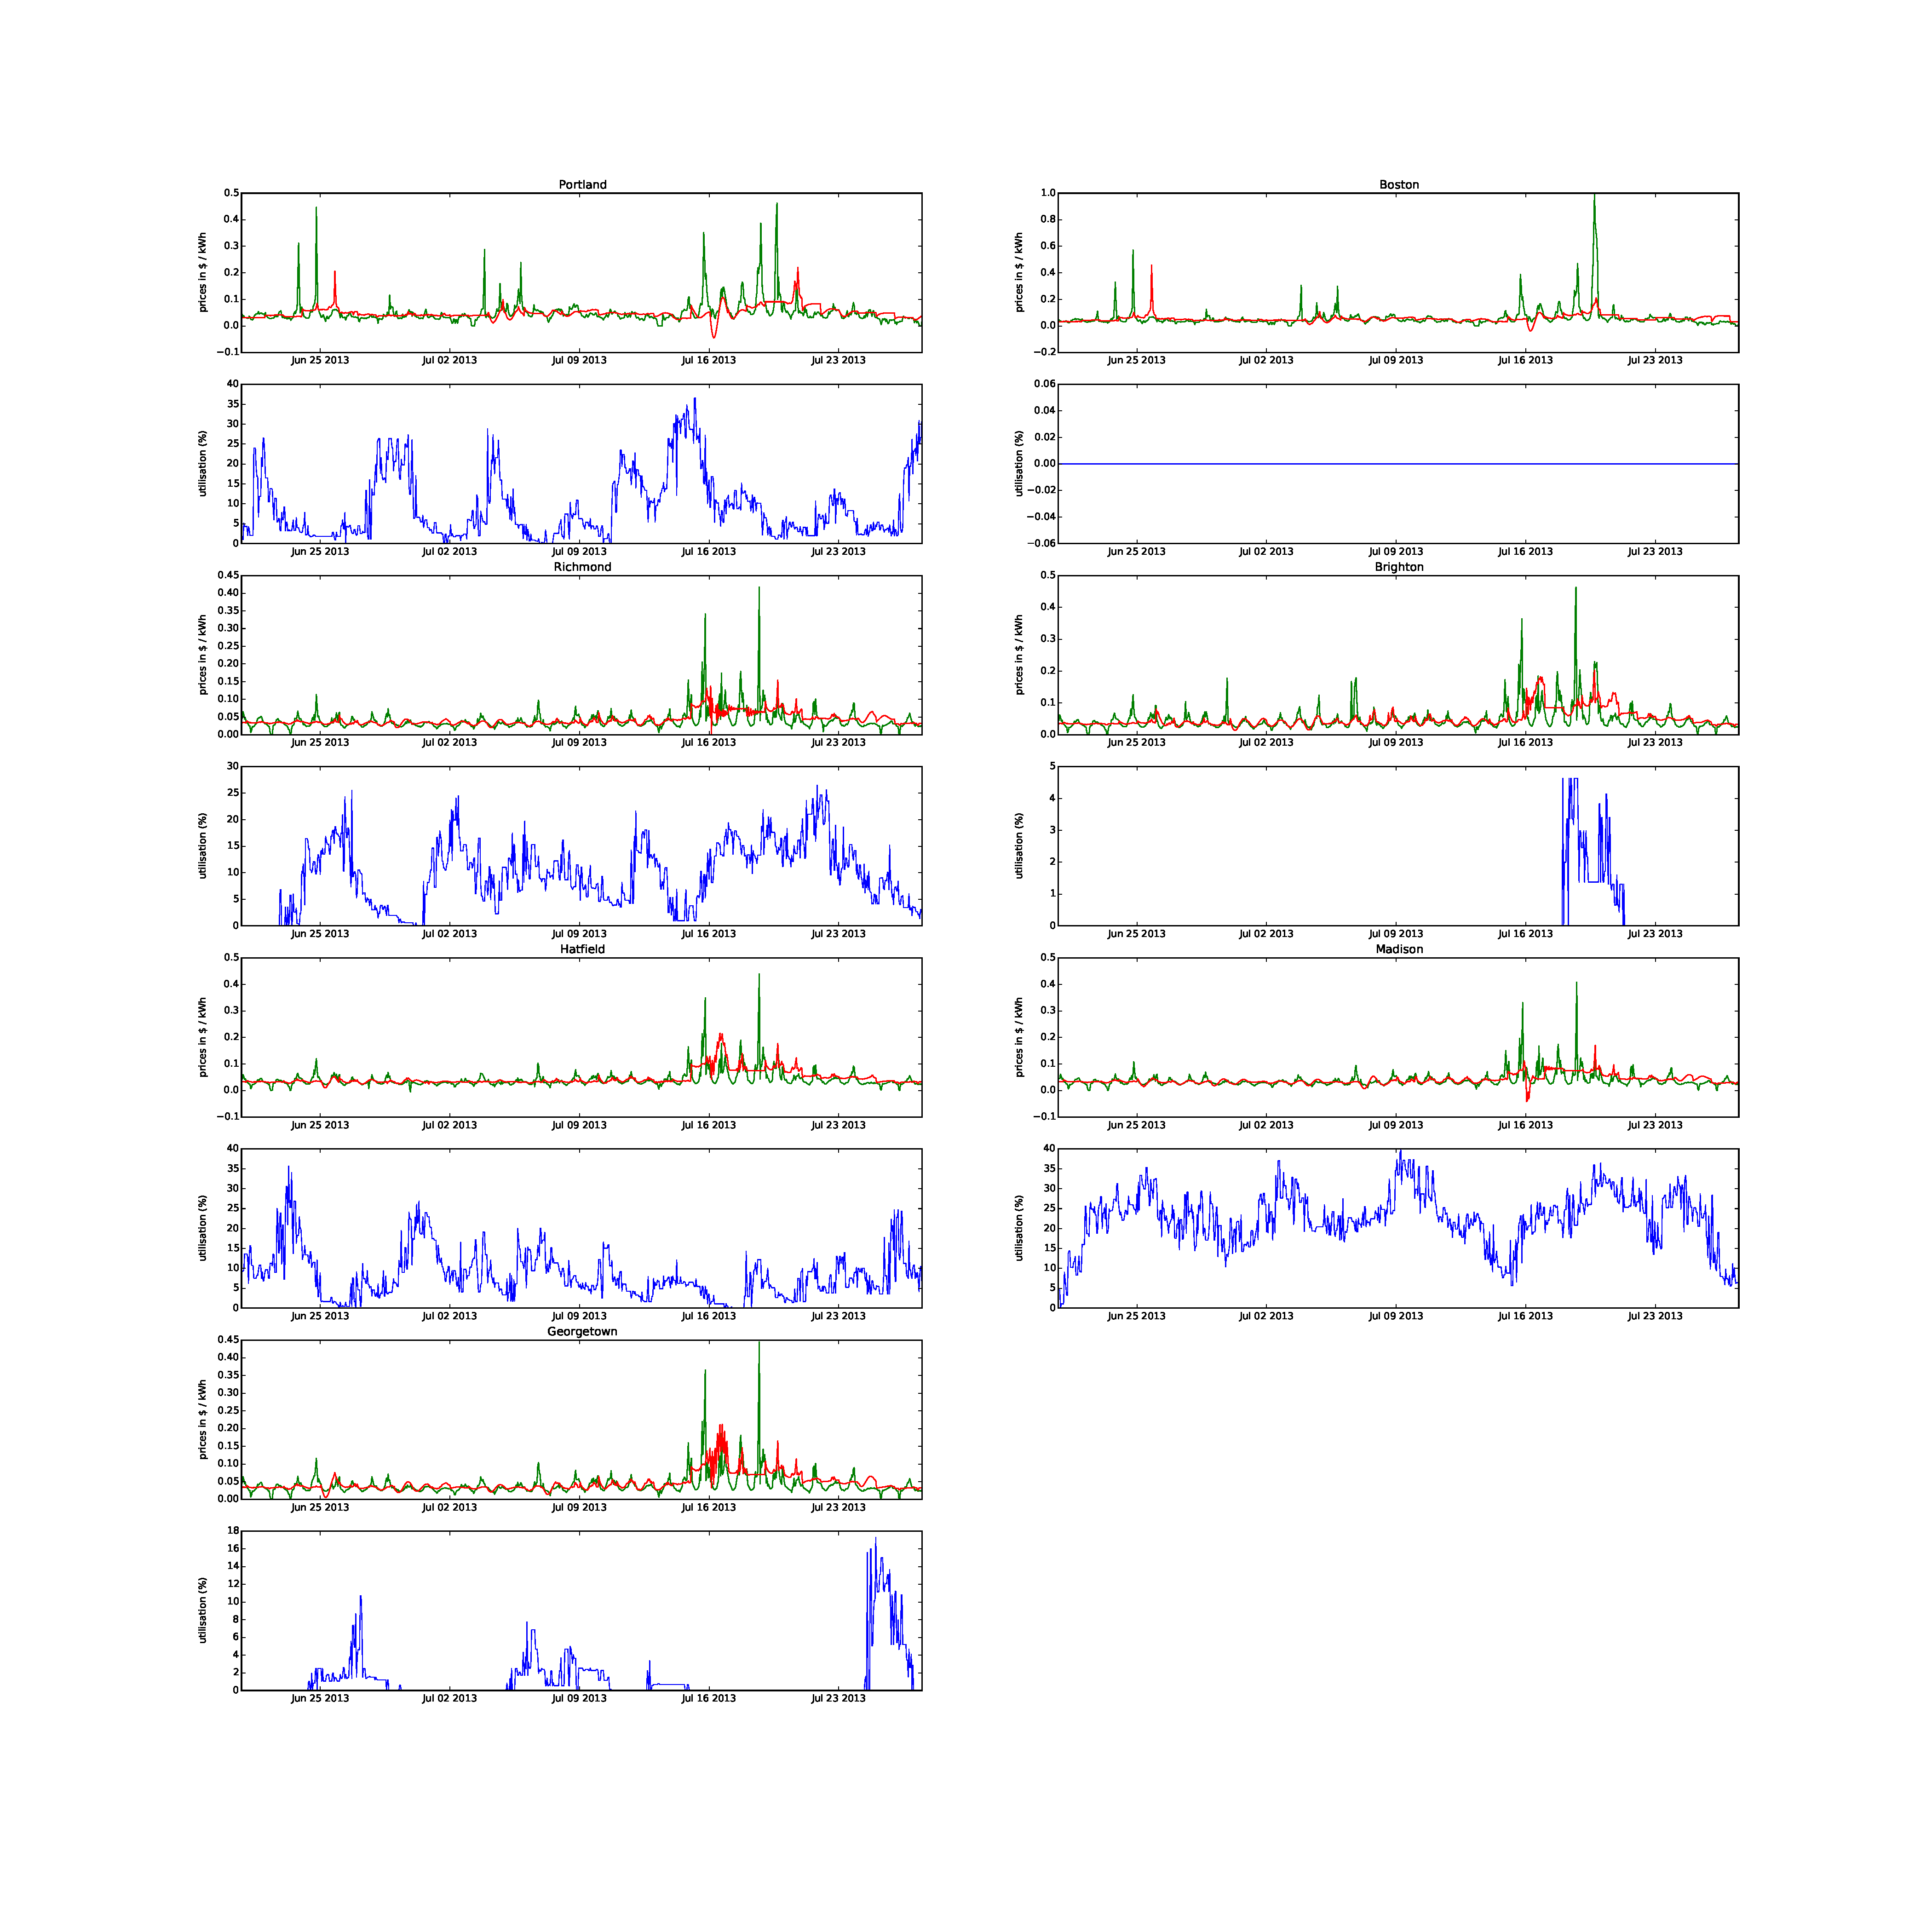
\includegraphics[width=1.60\textwidth]{figures/appendix_simulation_results/RT_Summer_scenario_2.pdf}
	\vspace*{-1.0in}
	\caption{Energy prices, energy price forecasts and utilization levels per location for simulation ``RT Summer'' and scheduler BCF}
	\label{fig:app_RT_Summer_scenario_2}
\end{figure}

\begin{figure}[htbp]
	\centering
	\vspace*{-0.6in}
	\hspace*{-1.4in}
		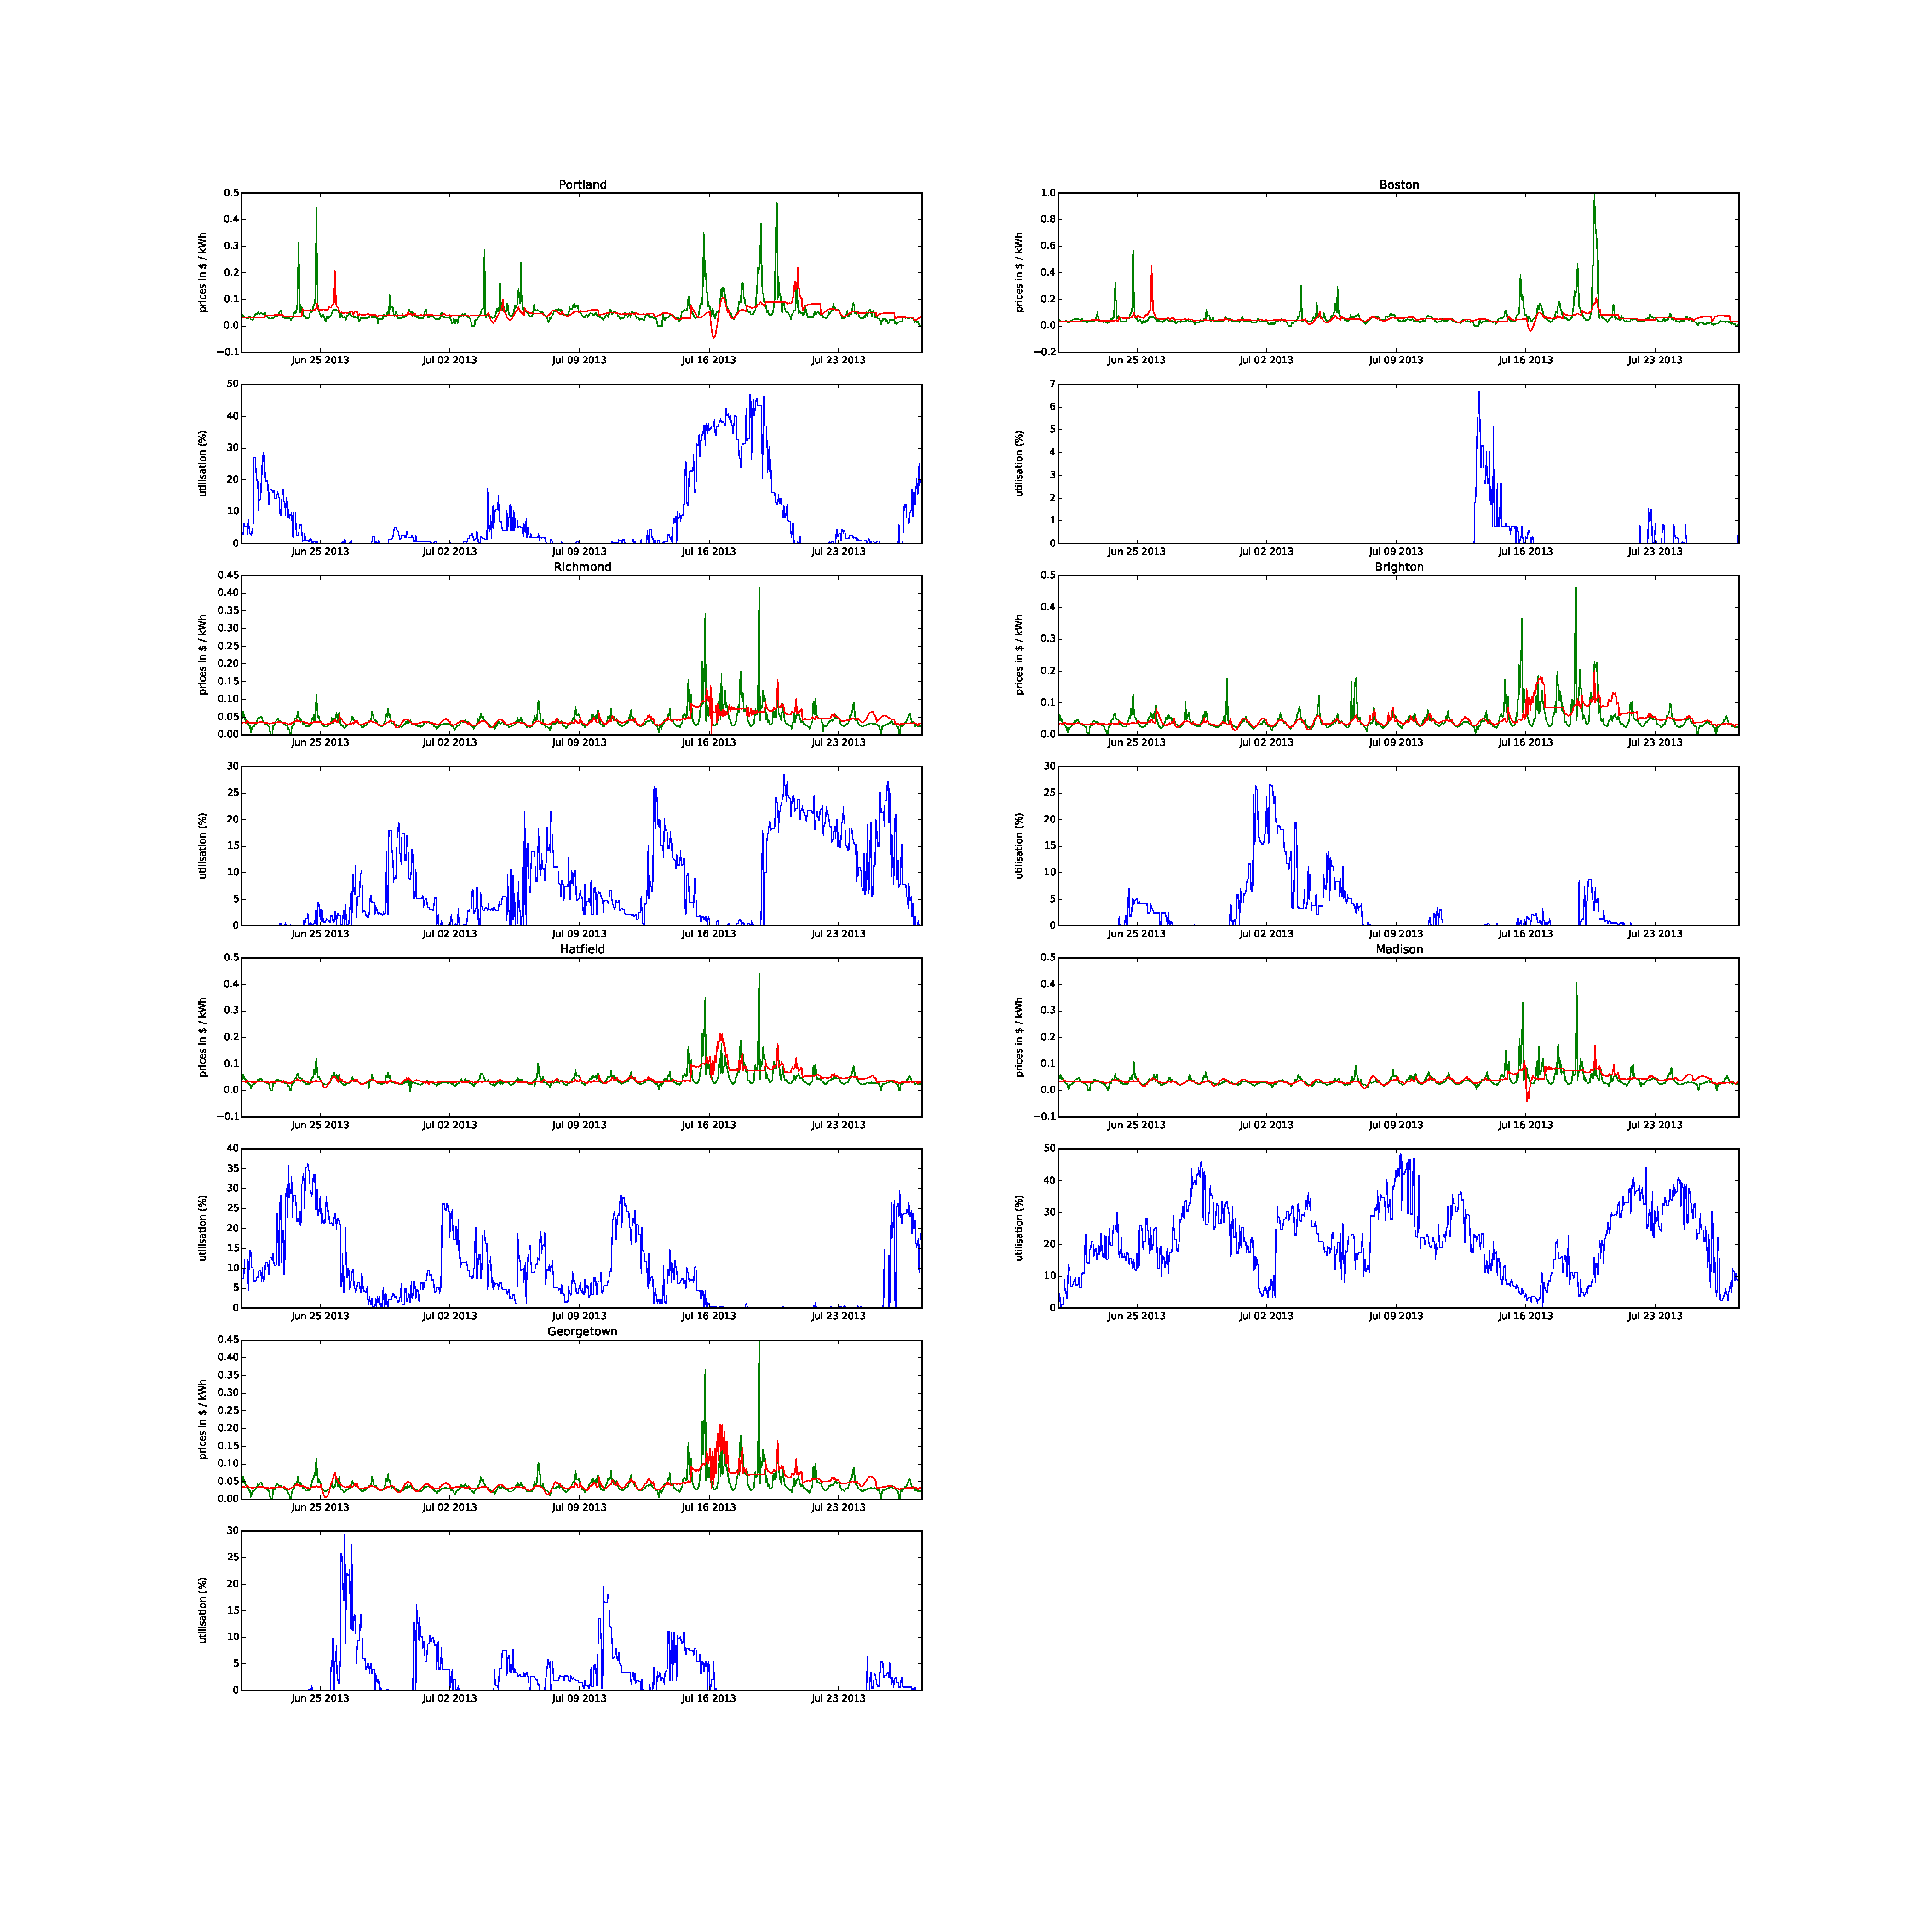
\includegraphics[width=1.60\textwidth]{figures/appendix_simulation_results/RT_Summer_scenario_3.pdf}
	\vspace*{-1.0in}
	\caption{Energy prices, energy price forecasts and utilization levels per location for simulation ``RT Summer'' and scheduler BCF\_F}
	\label{fig:app_RT_Summer_scenario_3}
\end{figure}

\begin{figure}[htbp]
	\centering
	\vspace*{-0.6in}
	\hspace*{-1.9in}
		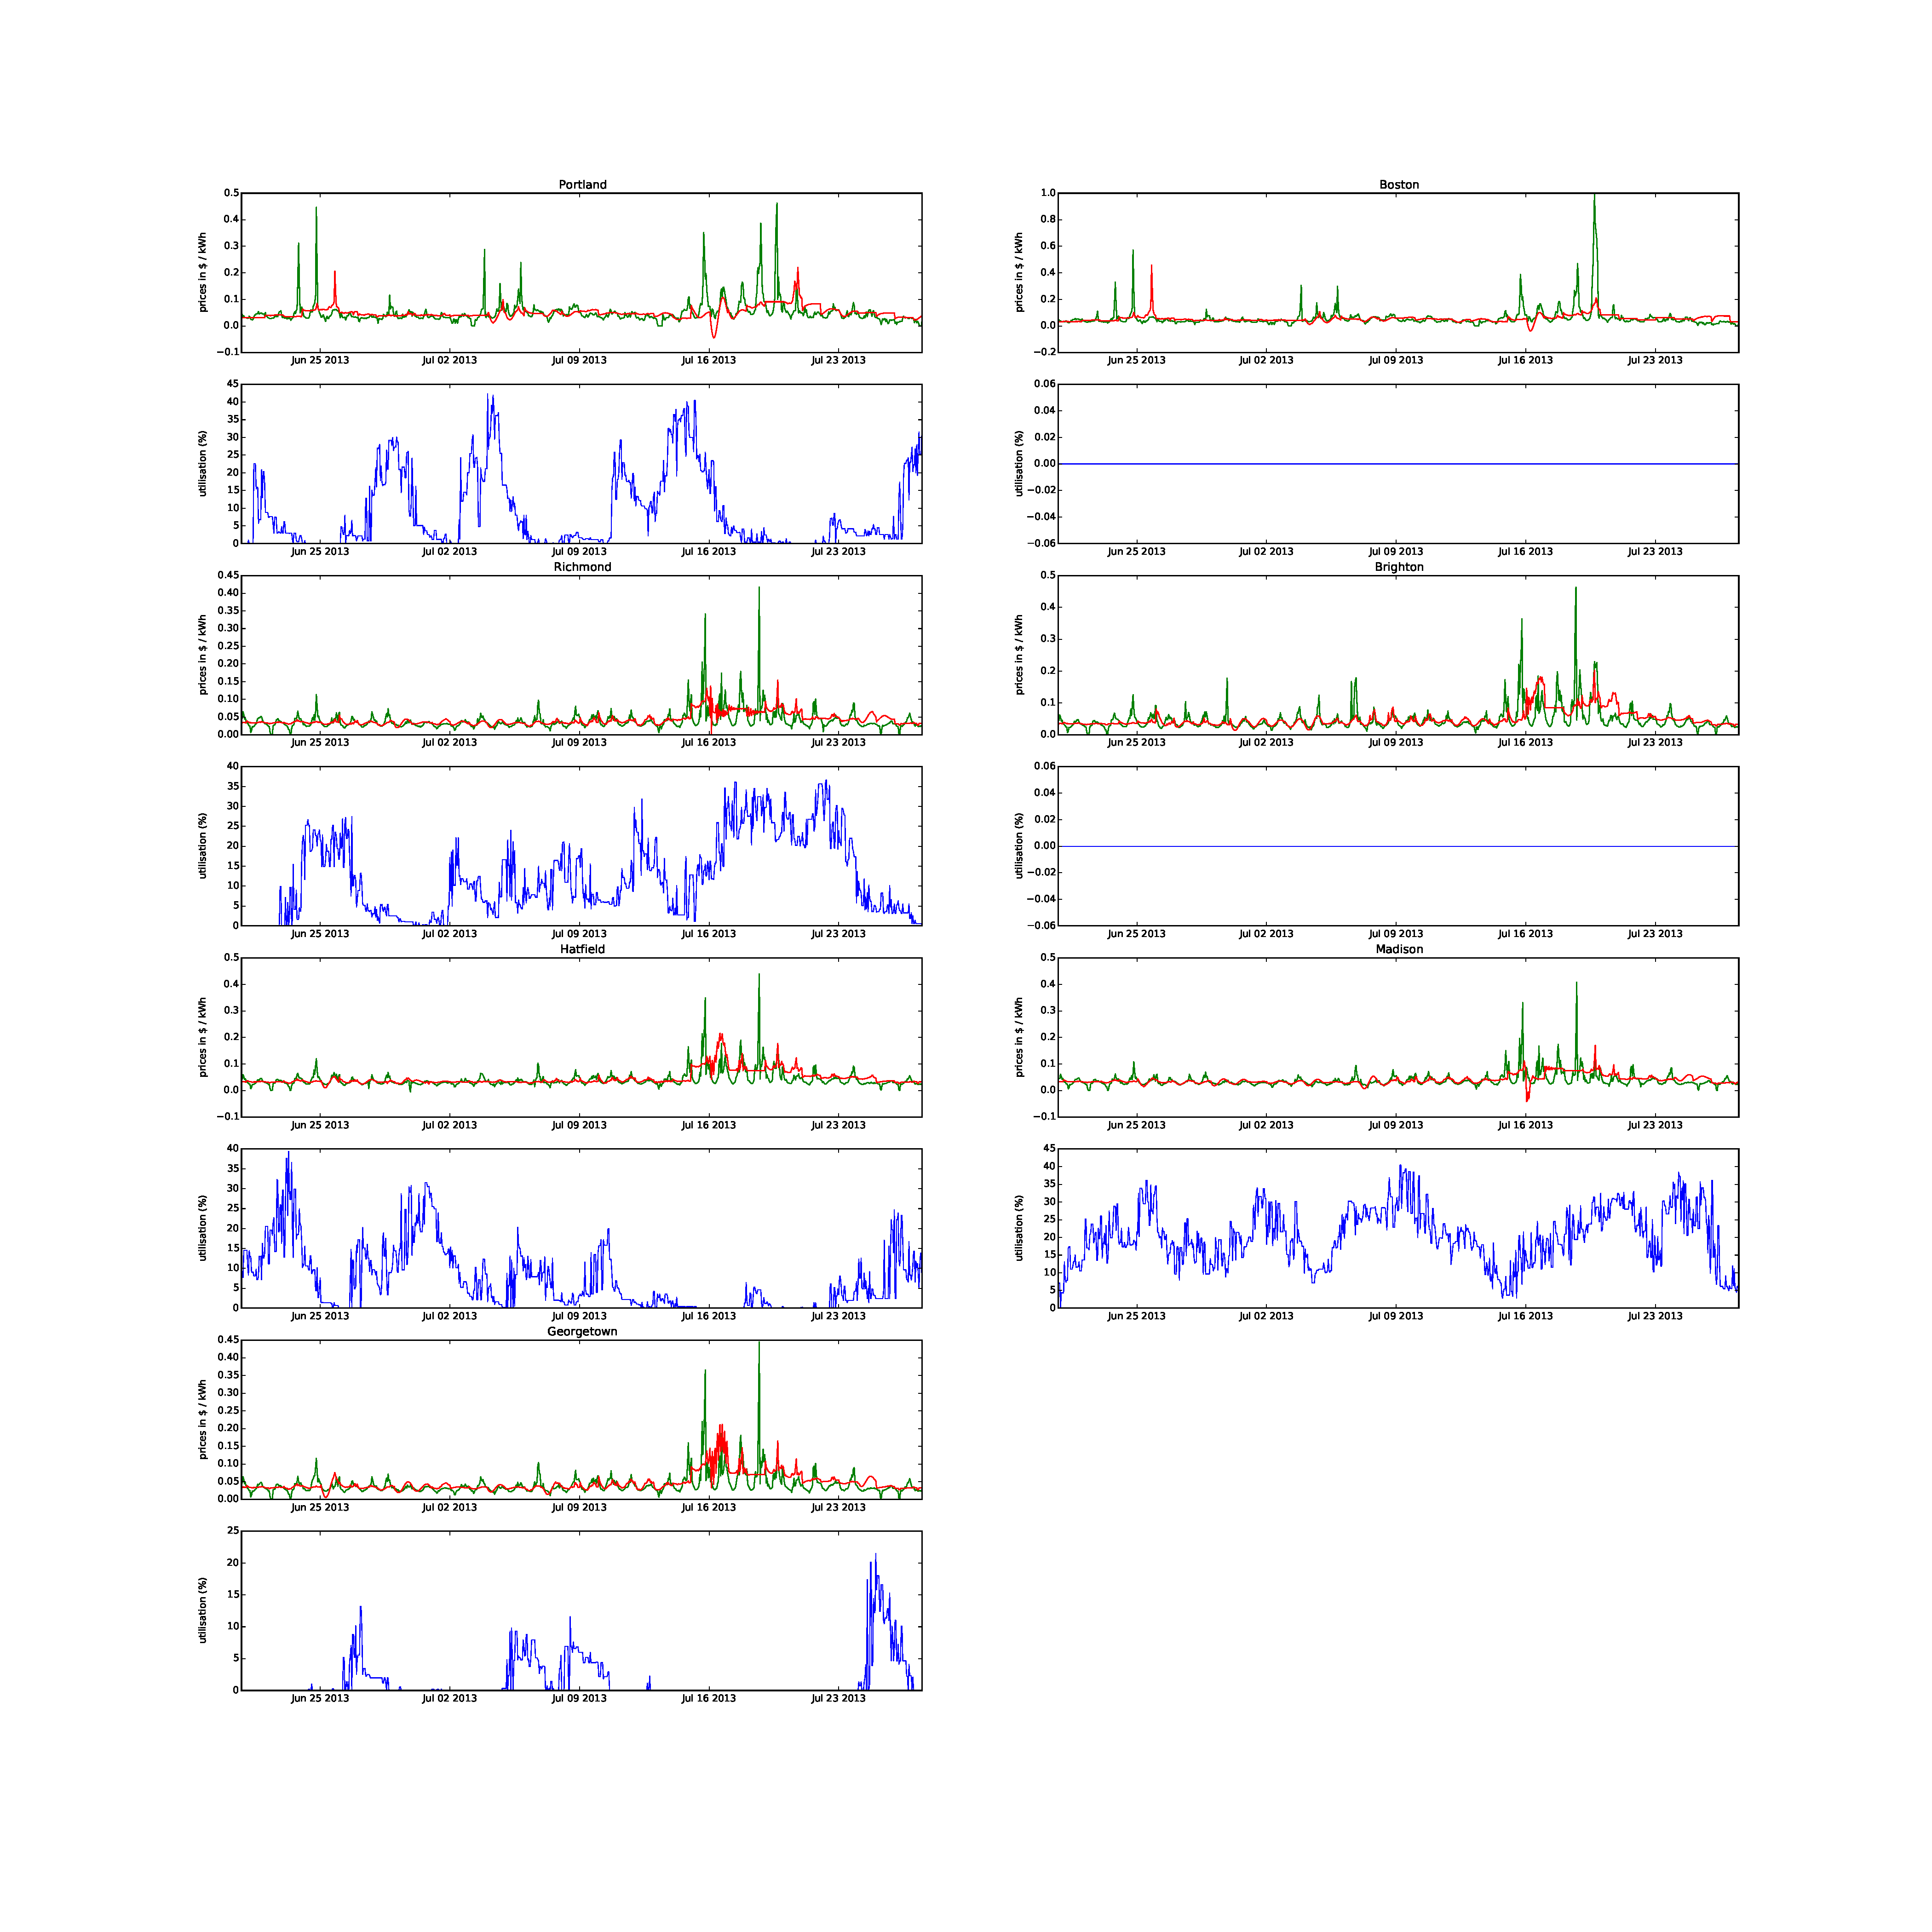
\includegraphics[width=1.60\textwidth]{figures/appendix_simulation_results/RT_Summer_scenario_4.pdf}
	\vspace*{-1.0in}
	\caption{Energy prices, energy price forecasts and utilization levels per location for simulation ``RT Summer'' and scheduler BCF\_IF}
	\label{fig:app_RT_Summer_scenario_4}
\end{figure}

\begin{figure}[htbp]
	\centering
	\vspace*{-0.6in}
	\hspace*{-1.4in}
		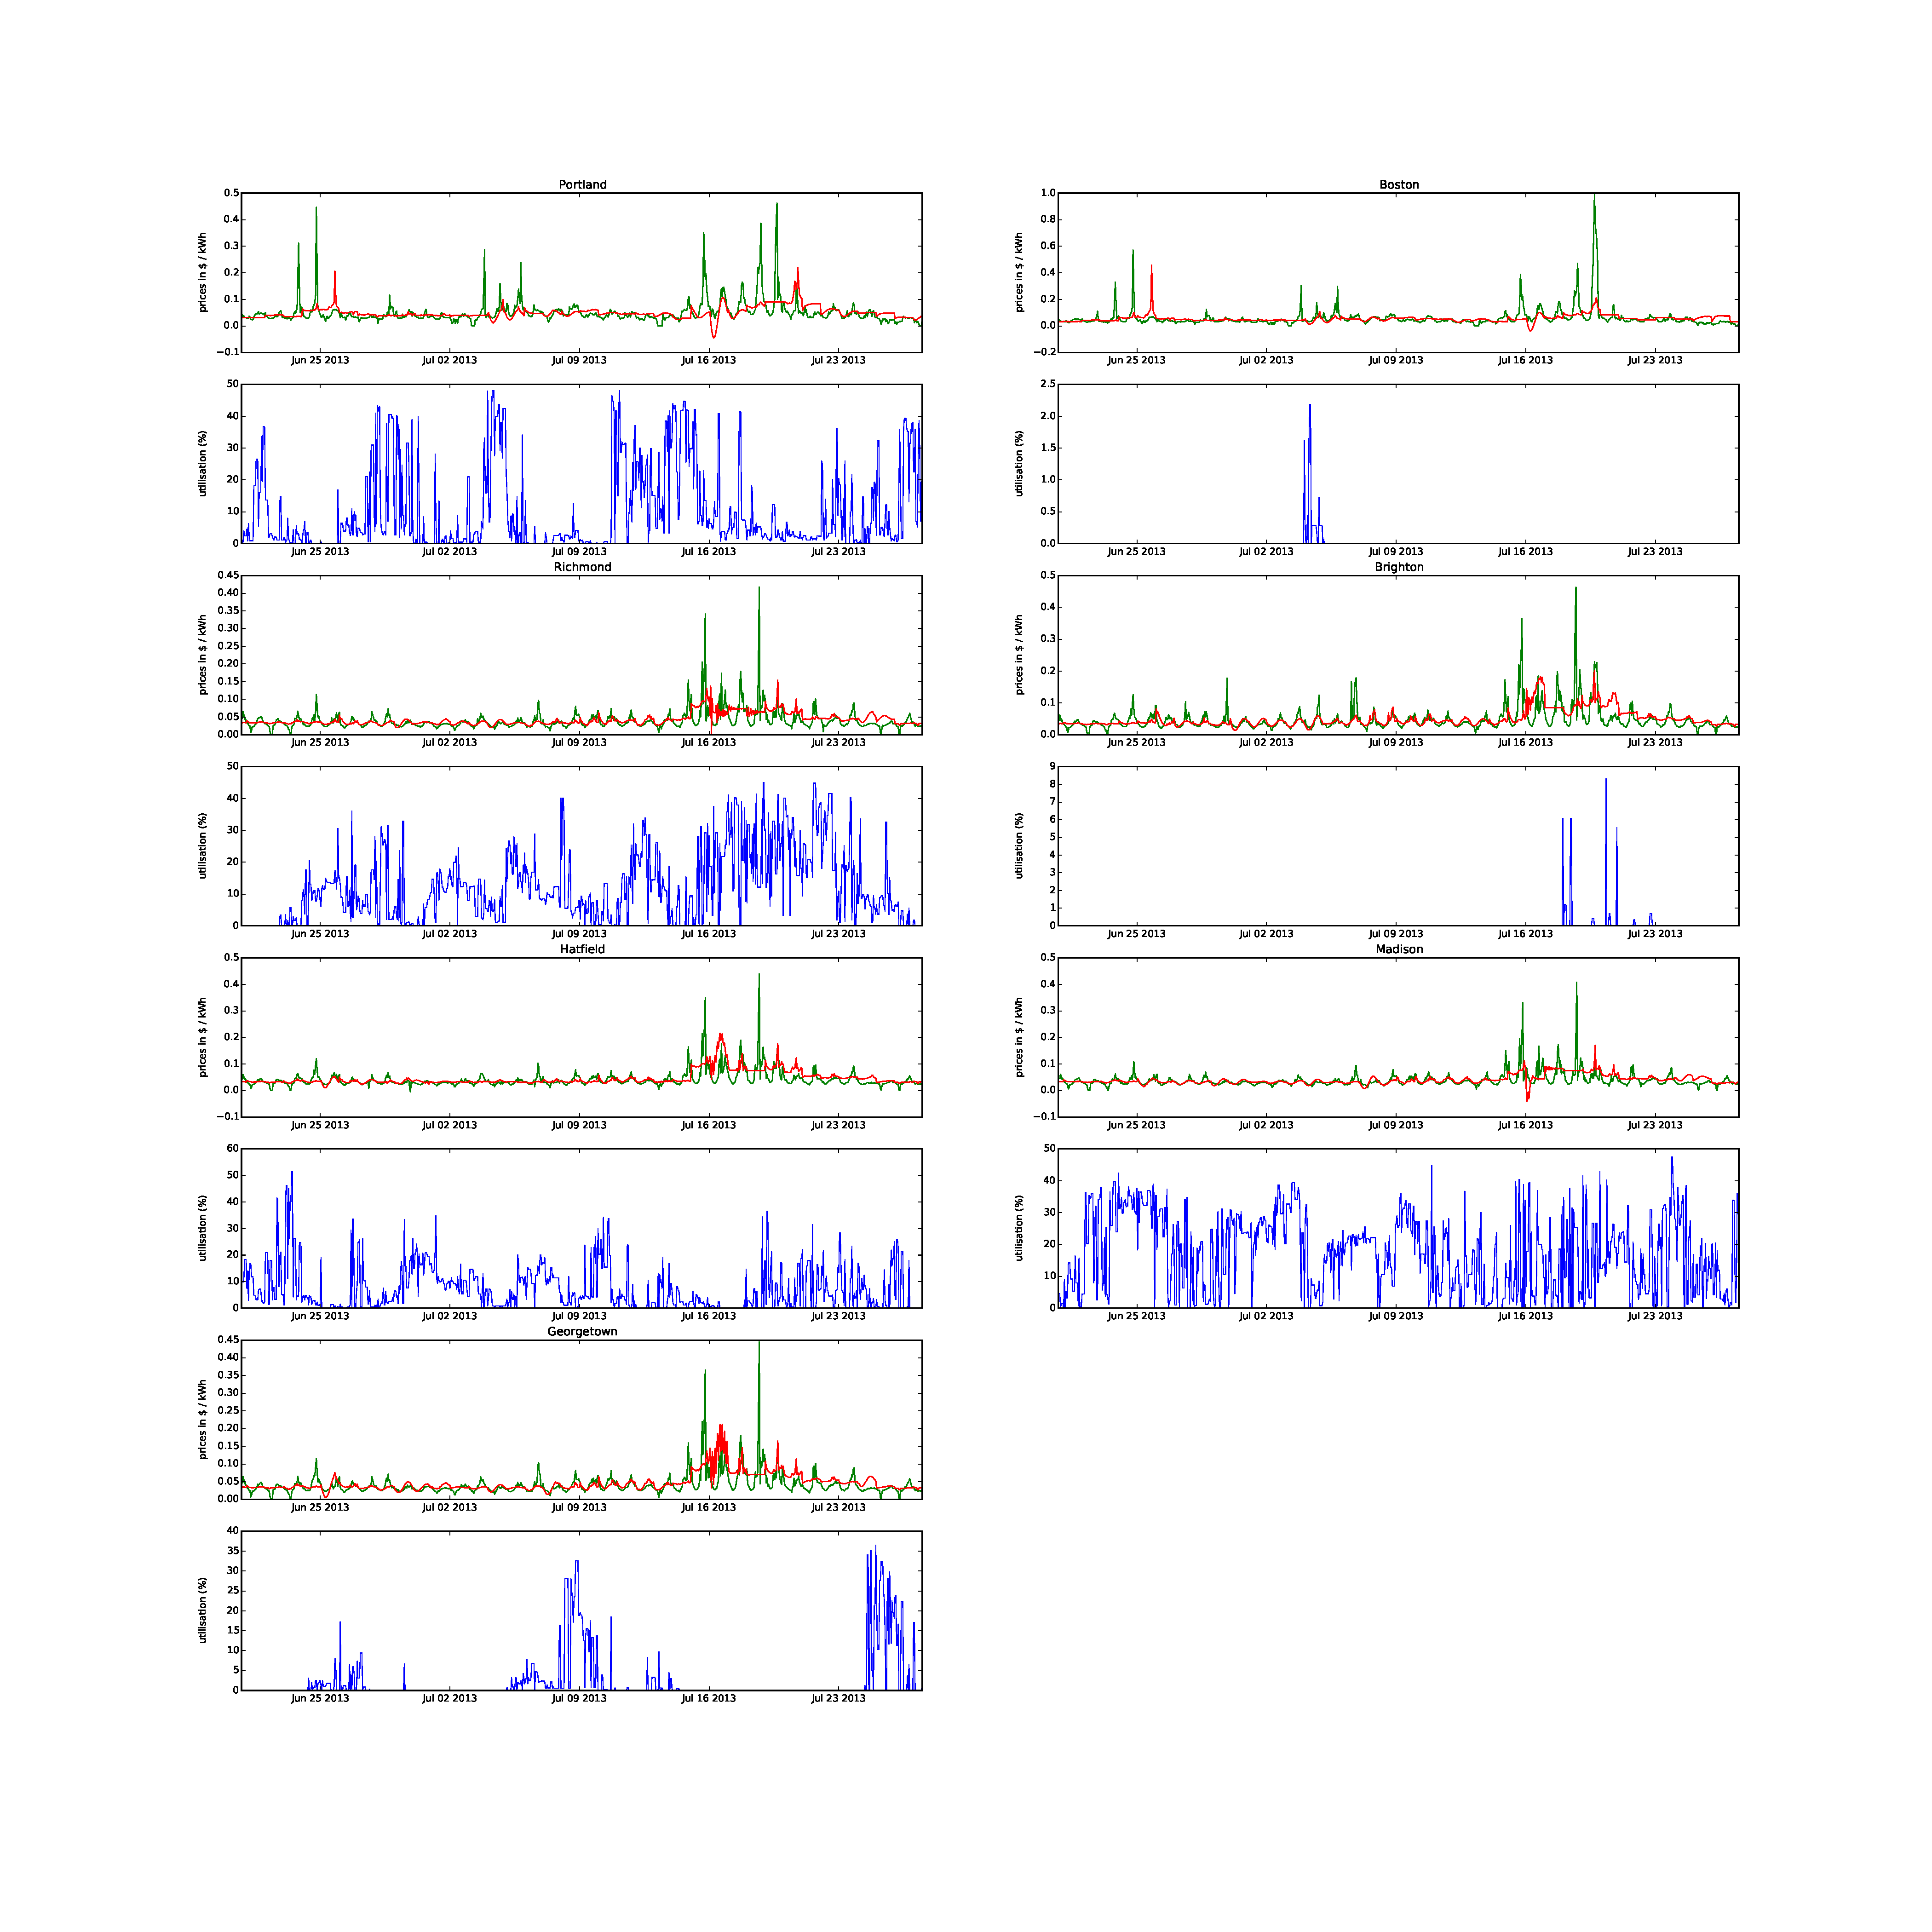
\includegraphics[width=1.60\textwidth]{figures/appendix_simulation_results/RT_Summer_scenario_5.pdf}
	\vspace*{-1.0in}
	\caption{Energy prices, energy price forecasts and utilization levels per location for simulation ``RT Summer'' and scheduler BCU\_M}
	\label{fig:app_RT_Summer_scenario_5}
\end{figure}

\begin{figure}[htbp]
	\centering
	\vspace*{-0.6in}
	\hspace*{-1.9in}
		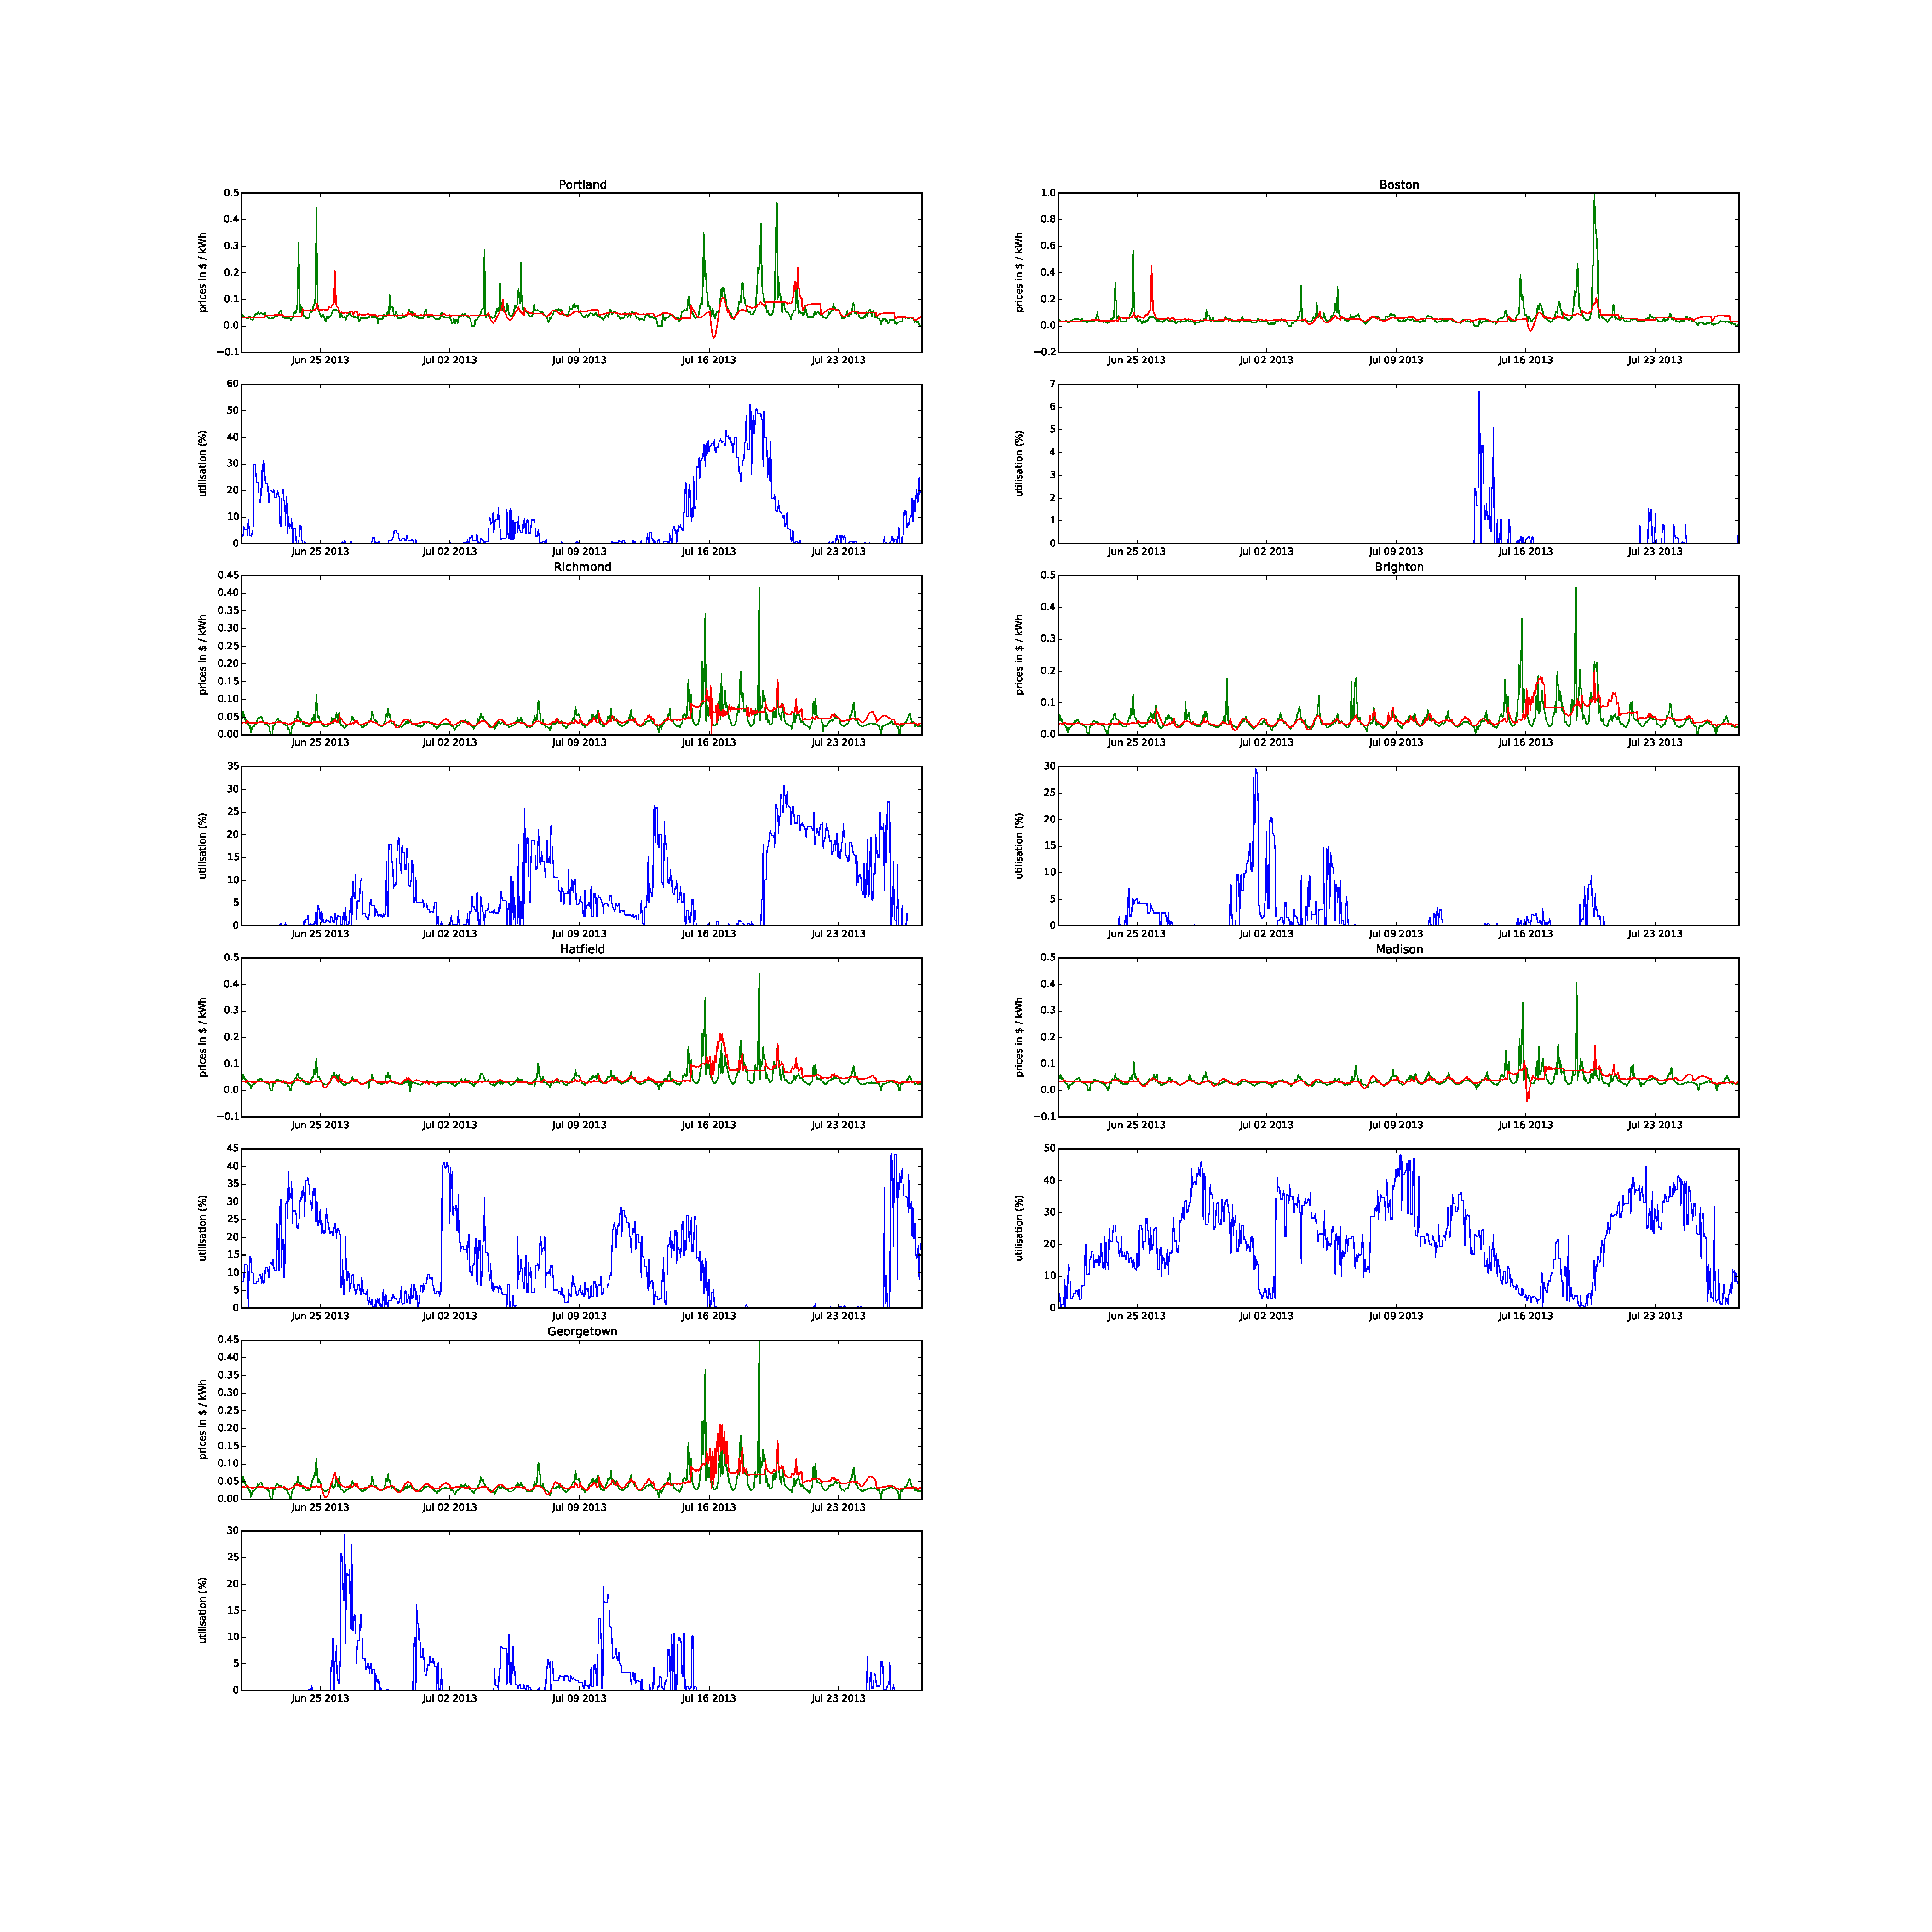
\includegraphics[width=1.60\textwidth]{figures/appendix_simulation_results/RT_Summer_scenario_6.pdf}
	\vspace*{-1.0in}
	\caption{Energy prices, energy price forecasts and utilization levels per location for simulation ``RT Summer'' and scheduler BCU\_MF}
	\label{fig:app_RT_Summer_scenario_6}
\end{figure}

\begin{figure}[htbp]
	\centering
	\vspace*{-0.6in}
	\hspace*{-1.4in}
		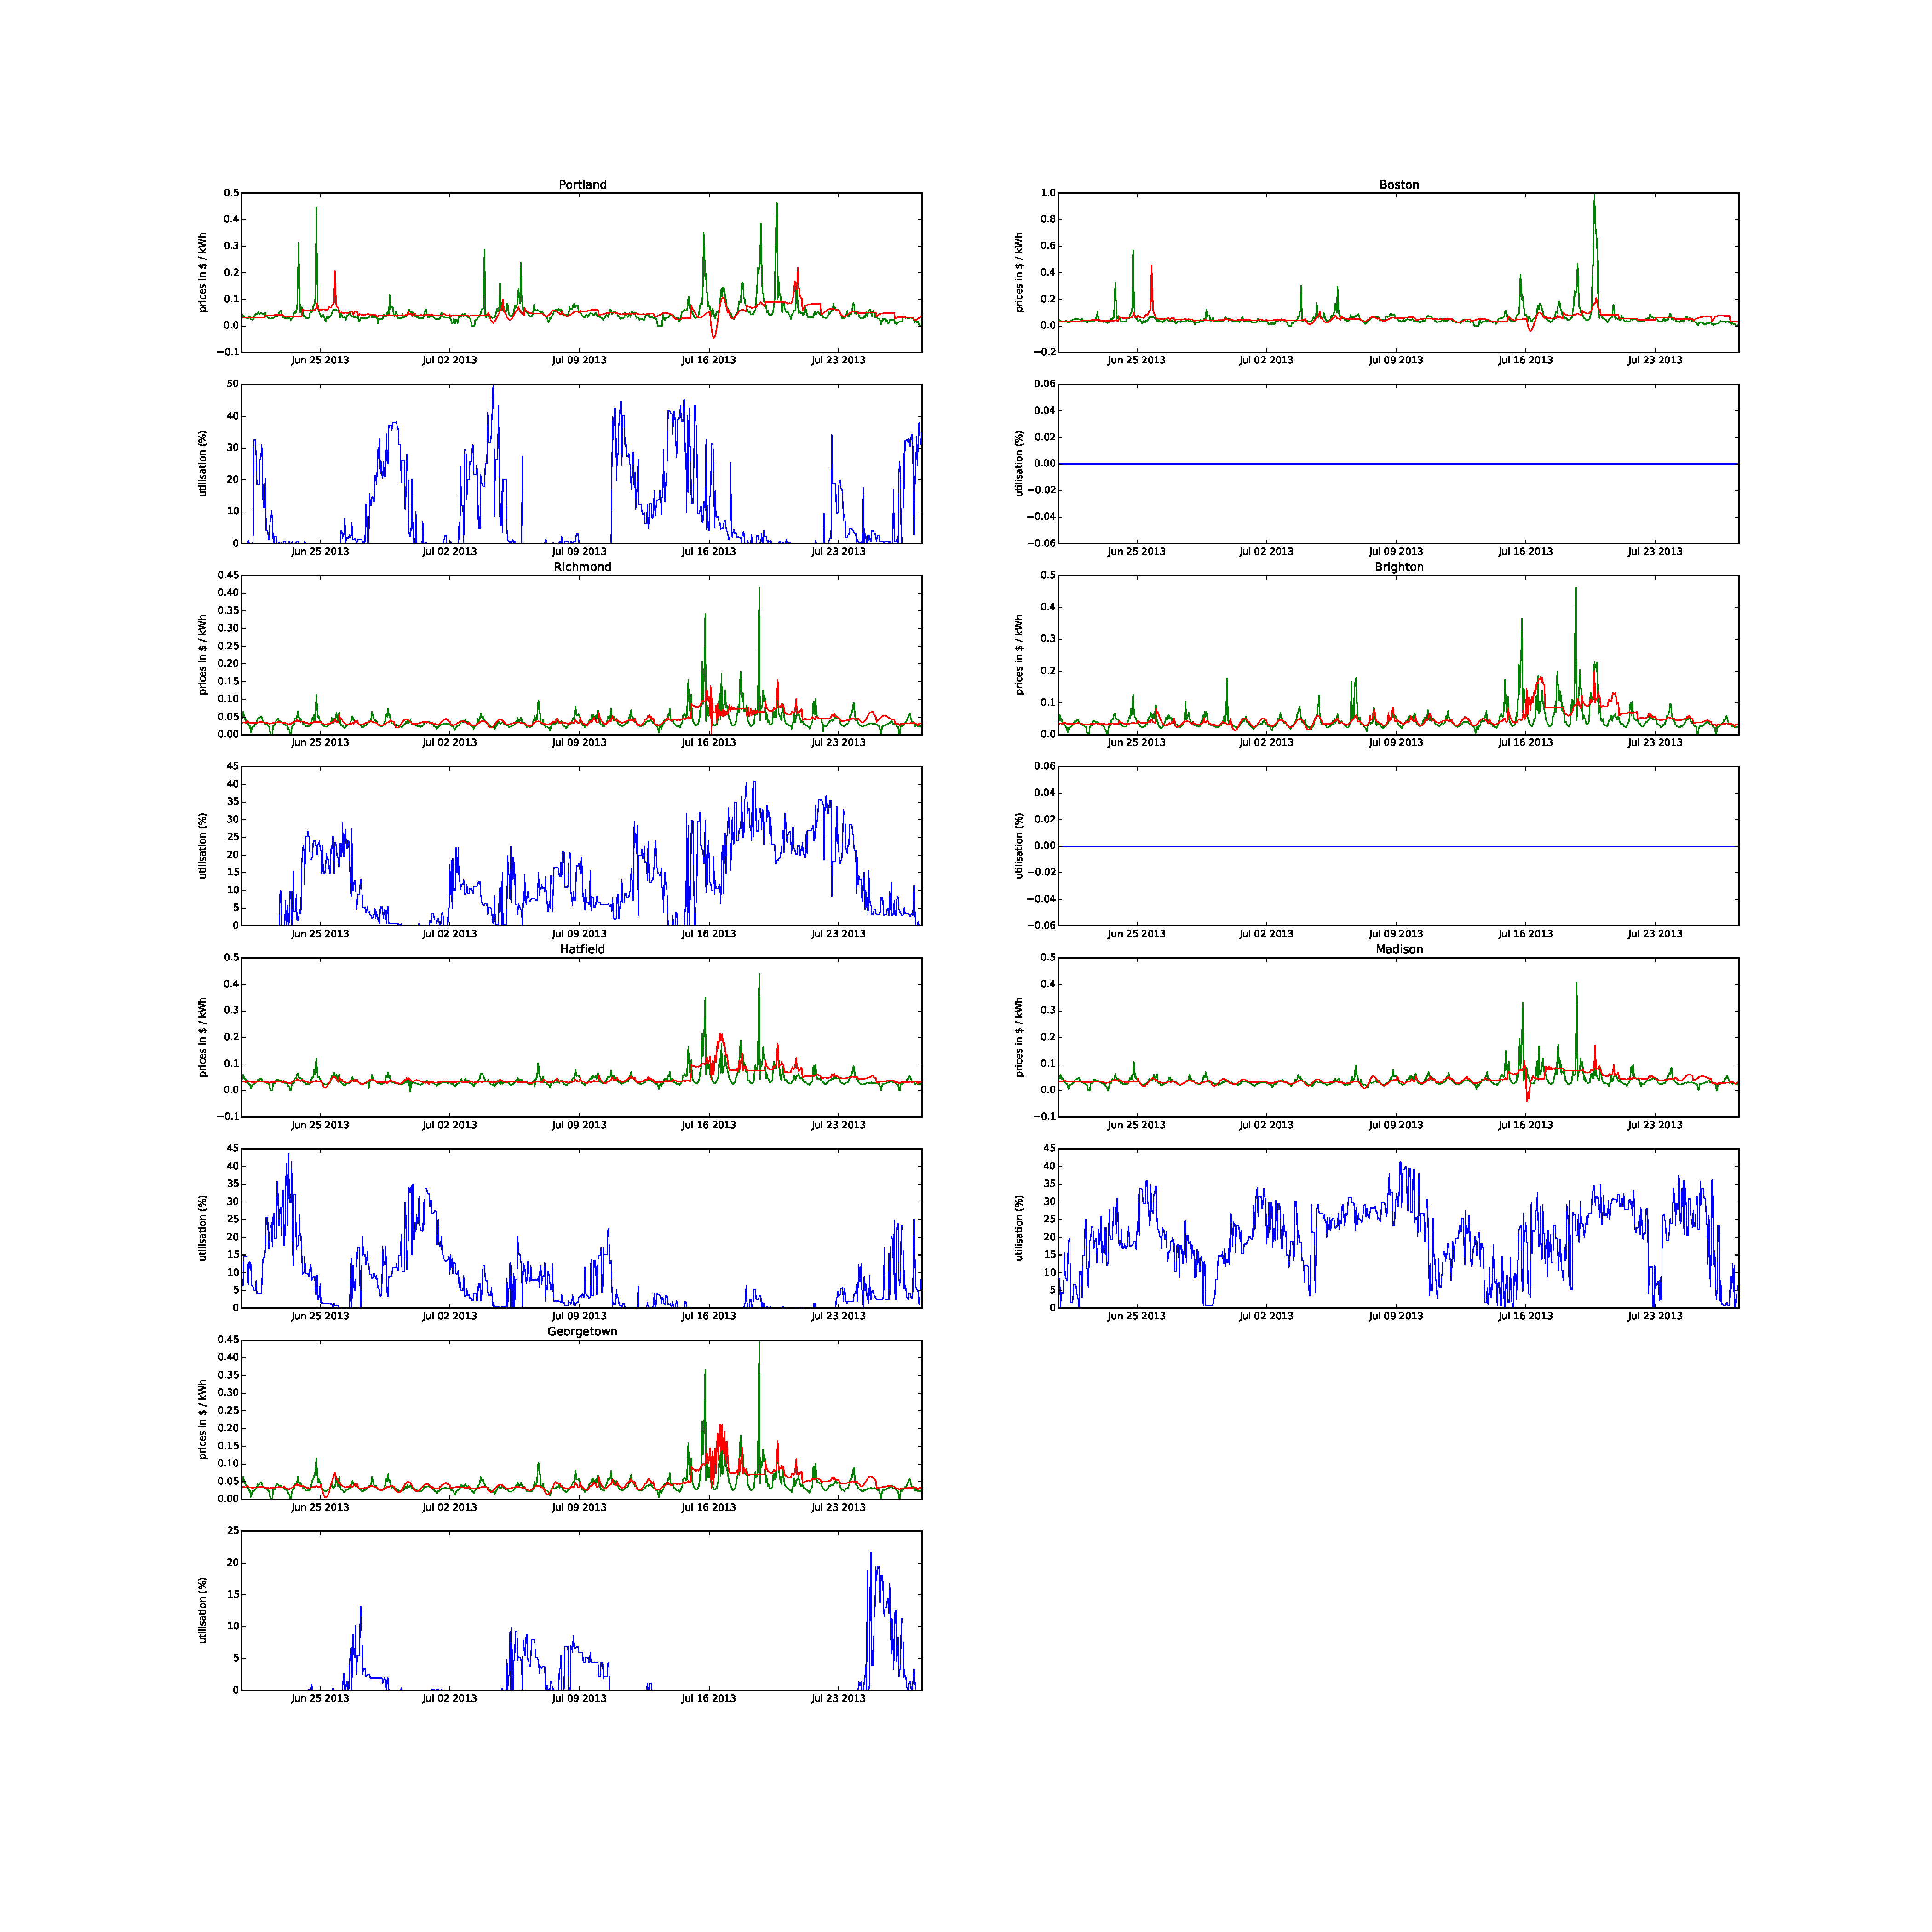
\includegraphics[width=1.60\textwidth]{figures/appendix_simulation_results/RT_Summer_scenario_7.pdf}
	\vspace*{-1.0in}
	\caption{Energy prices, energy price forecasts and utilization levels per location for simulation ``RT Summer'' and scheduler BCU\_MIF}
	\label{fig:app_RT_Summer_scenario_7}
\end{figure}


\FloatBarrier
\subsection{Simulation results for RT Spring}

\begin{figure}[htbp]
	\centering
	\vspace*{-0.6in}
	\hspace*{-1.4in}
		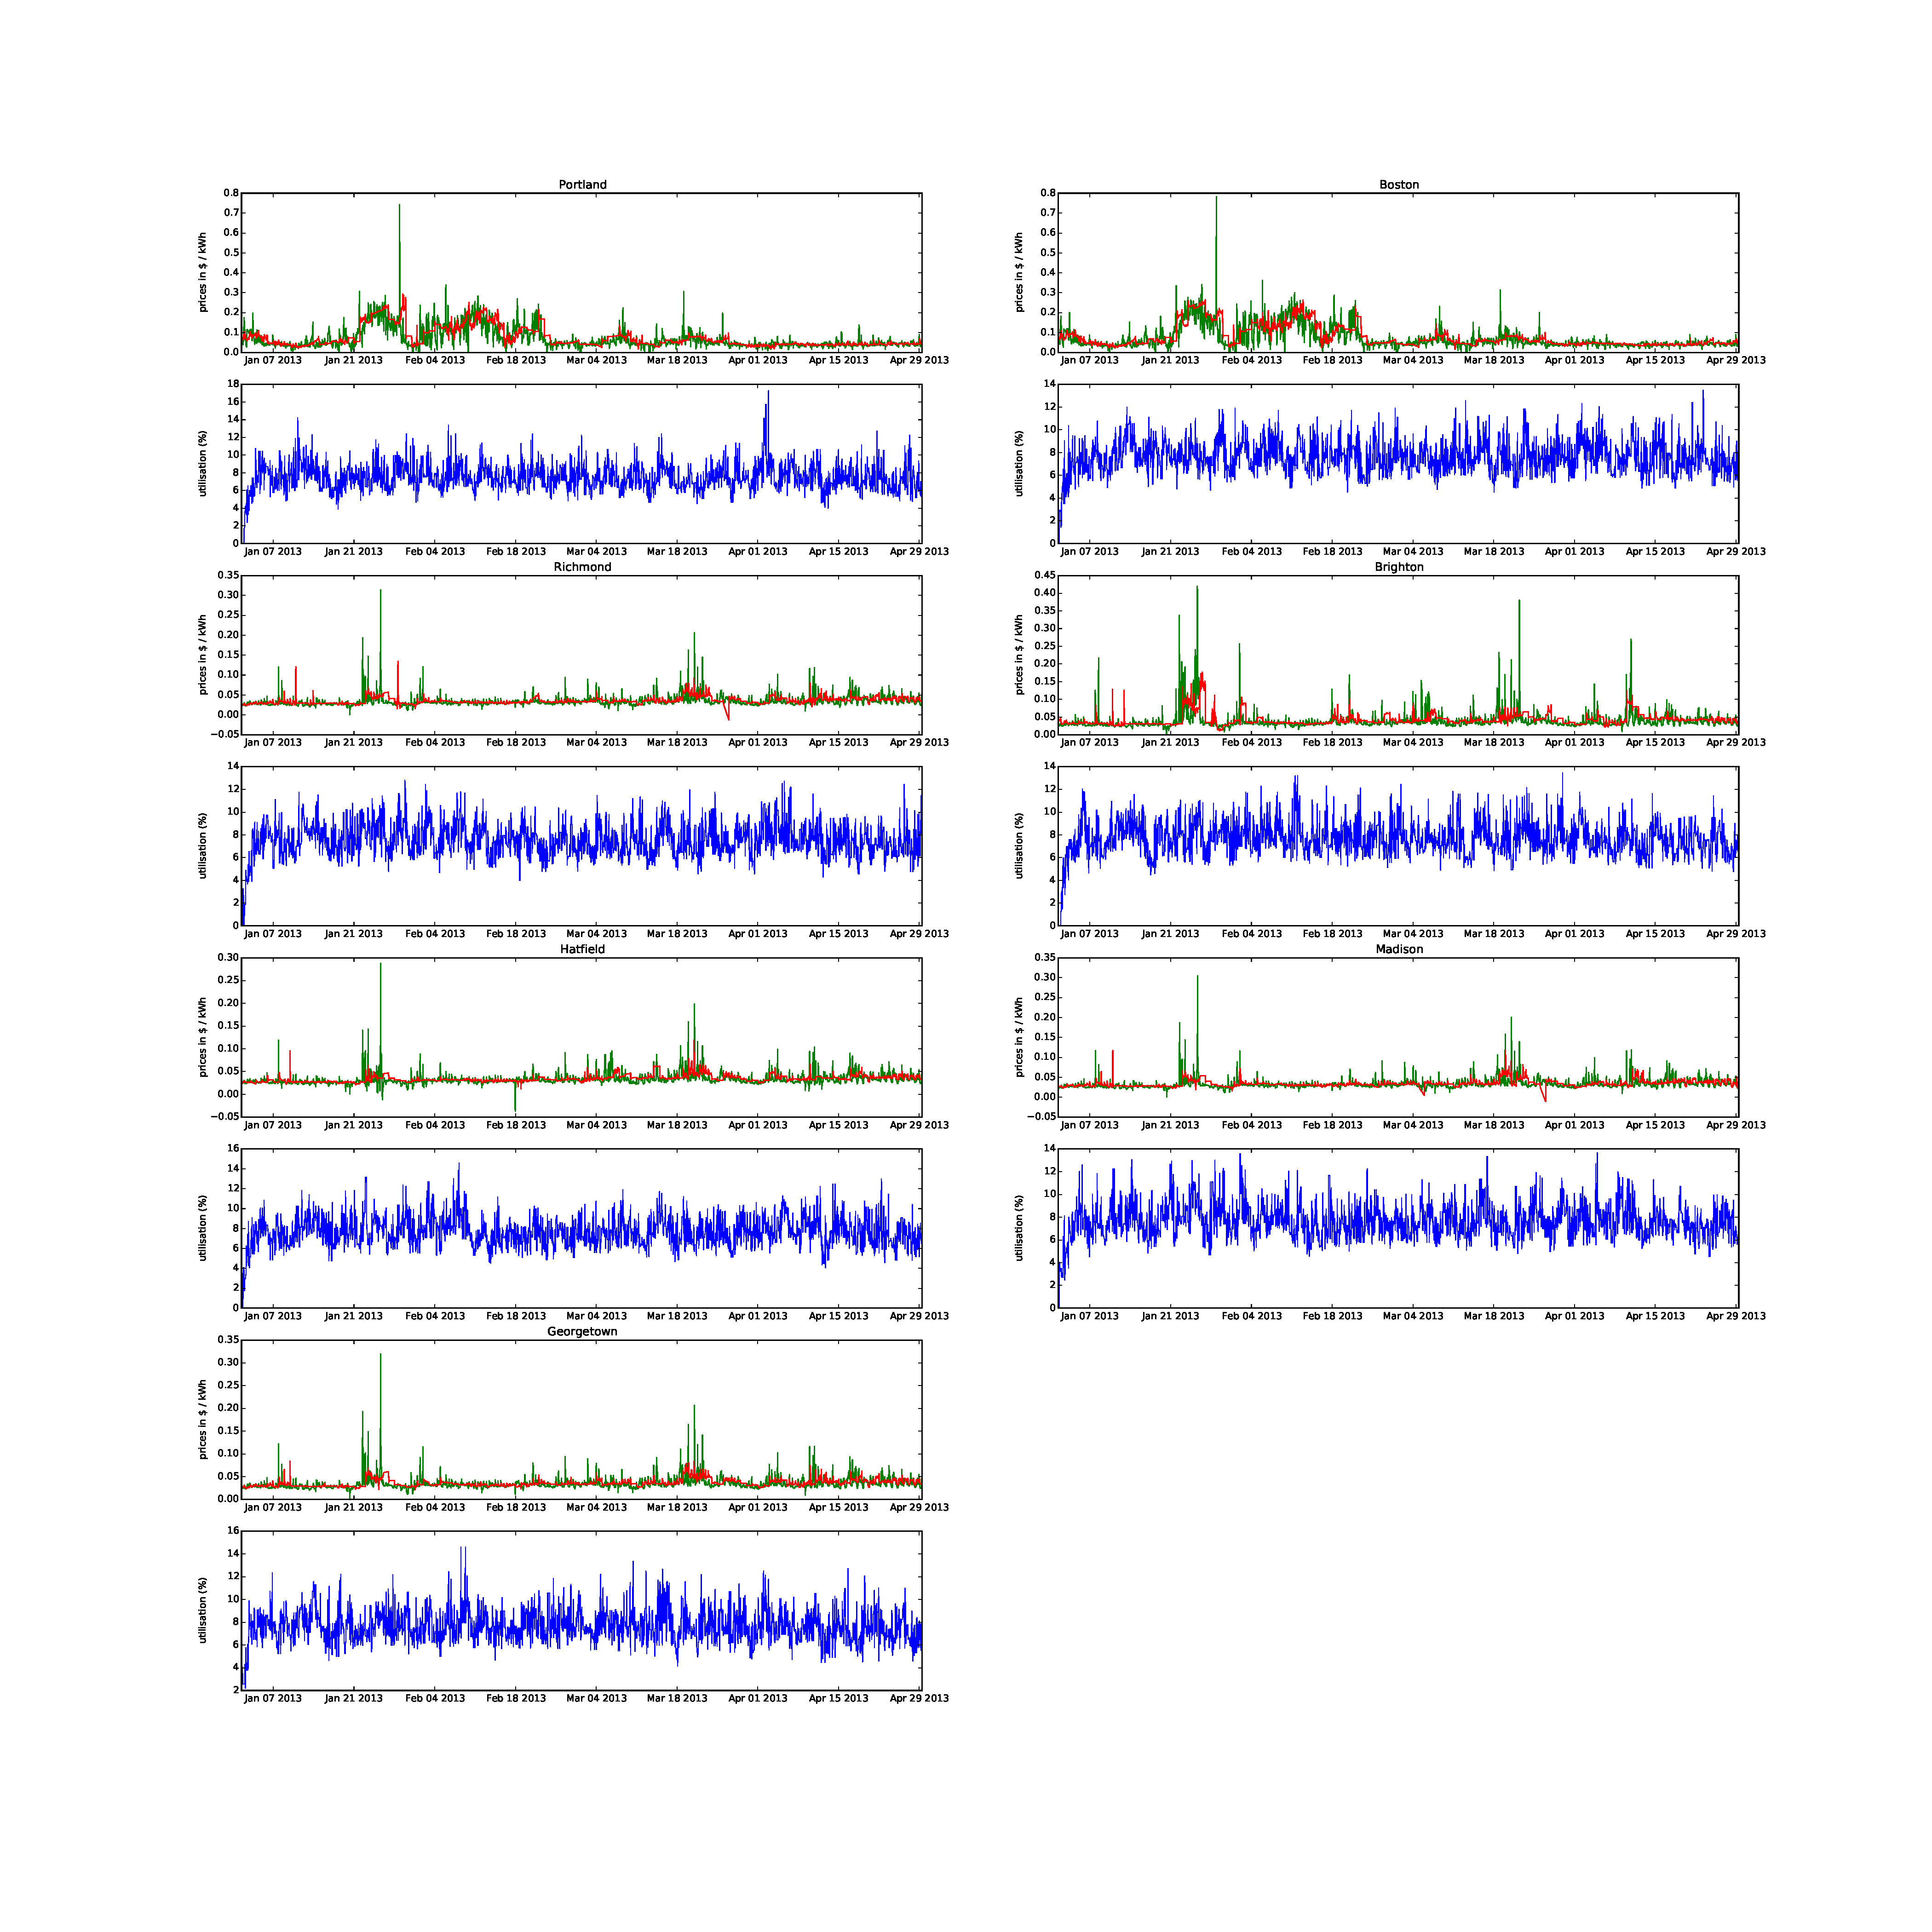
\includegraphics[width=1.60\textwidth]{figures/appendix_simulation_results/RT_Spring_scenario_1.pdf}
	\vspace*{-1.0in}
	\caption{Energy prices, energy price forecasts and utilization levels per location for simulation ``RT Spring'' and scheduler BFD}
	\label{fig:app_RT_Spring_scenario_1}
\end{figure}

\begin{figure}[htbp]
	\centering
	\vspace*{-0.6in}
	\hspace*{-1.9in}
		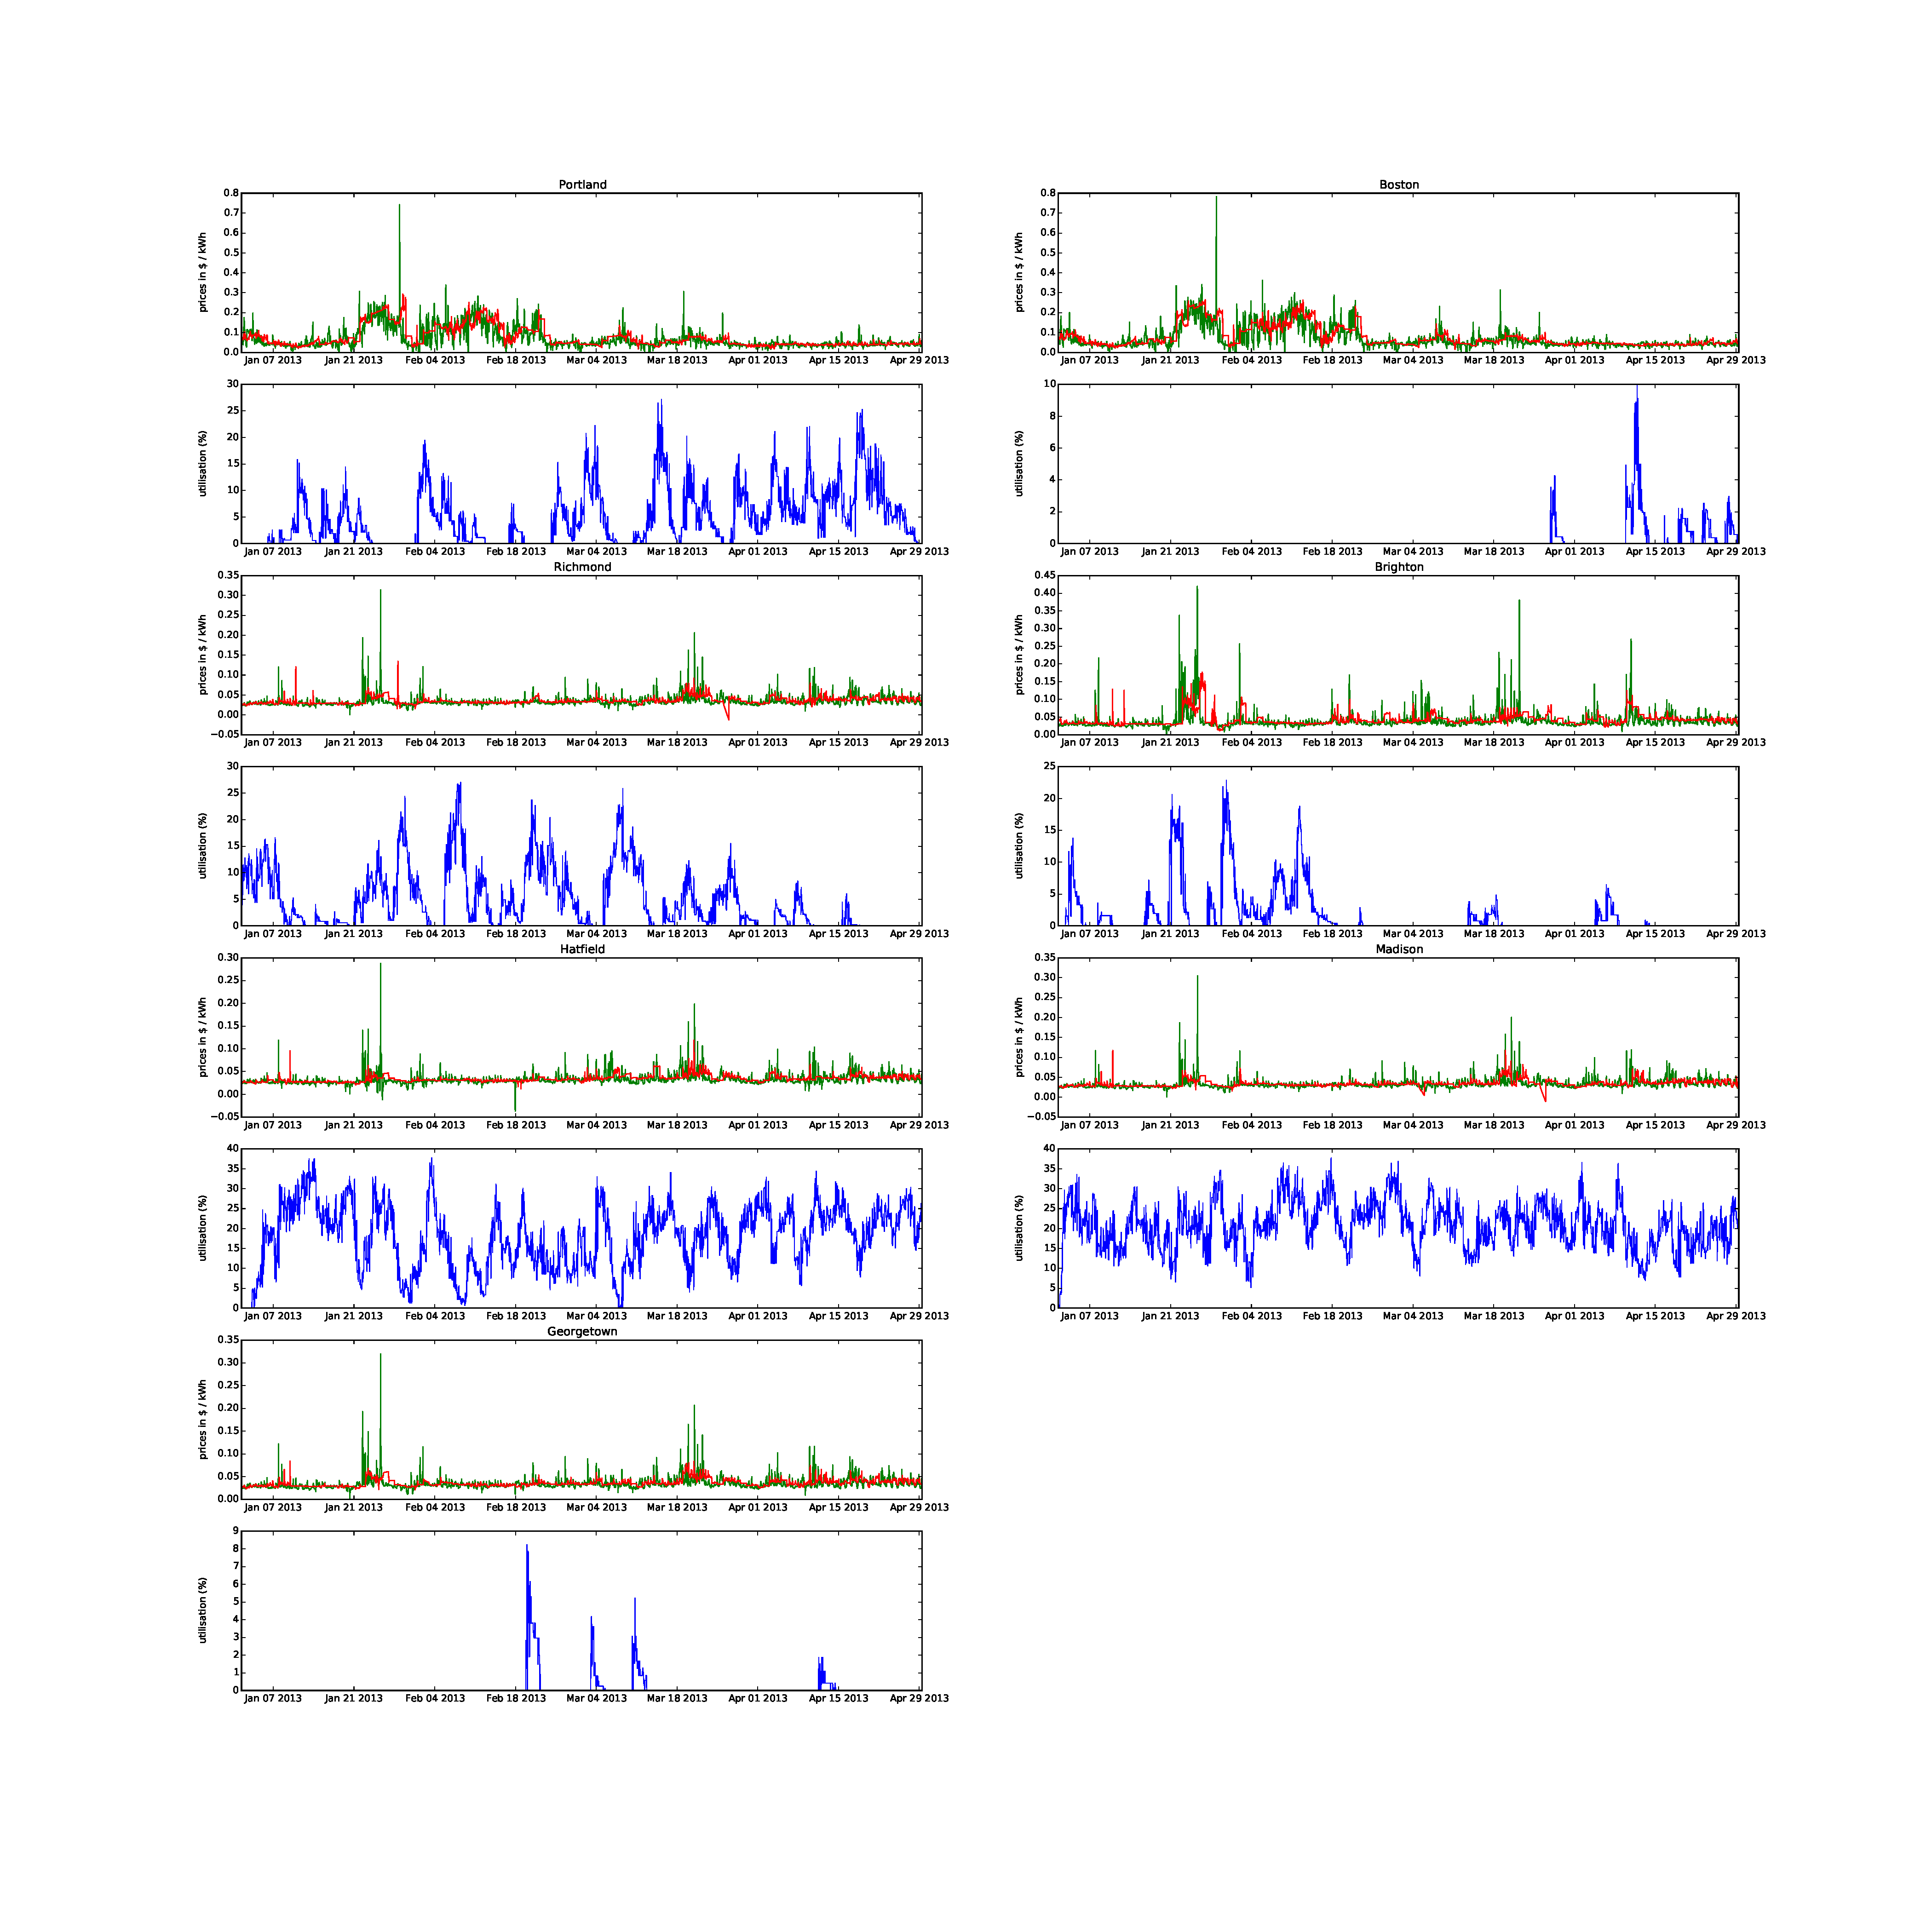
\includegraphics[width=1.60\textwidth]{figures/appendix_simulation_results/RT_Spring_scenario_2.pdf}
	\vspace*{-1.0in}
	\caption{Energy prices, energy price forecasts and utilization levels per location for simulation ``RT Spring'' and scheduler BCF}
	\label{fig:app_RT_Spring_scenario_2}
\end{figure}

\begin{figure}[htbp]
	\centering
	\vspace*{-0.6in}
	\hspace*{-1.4in}
		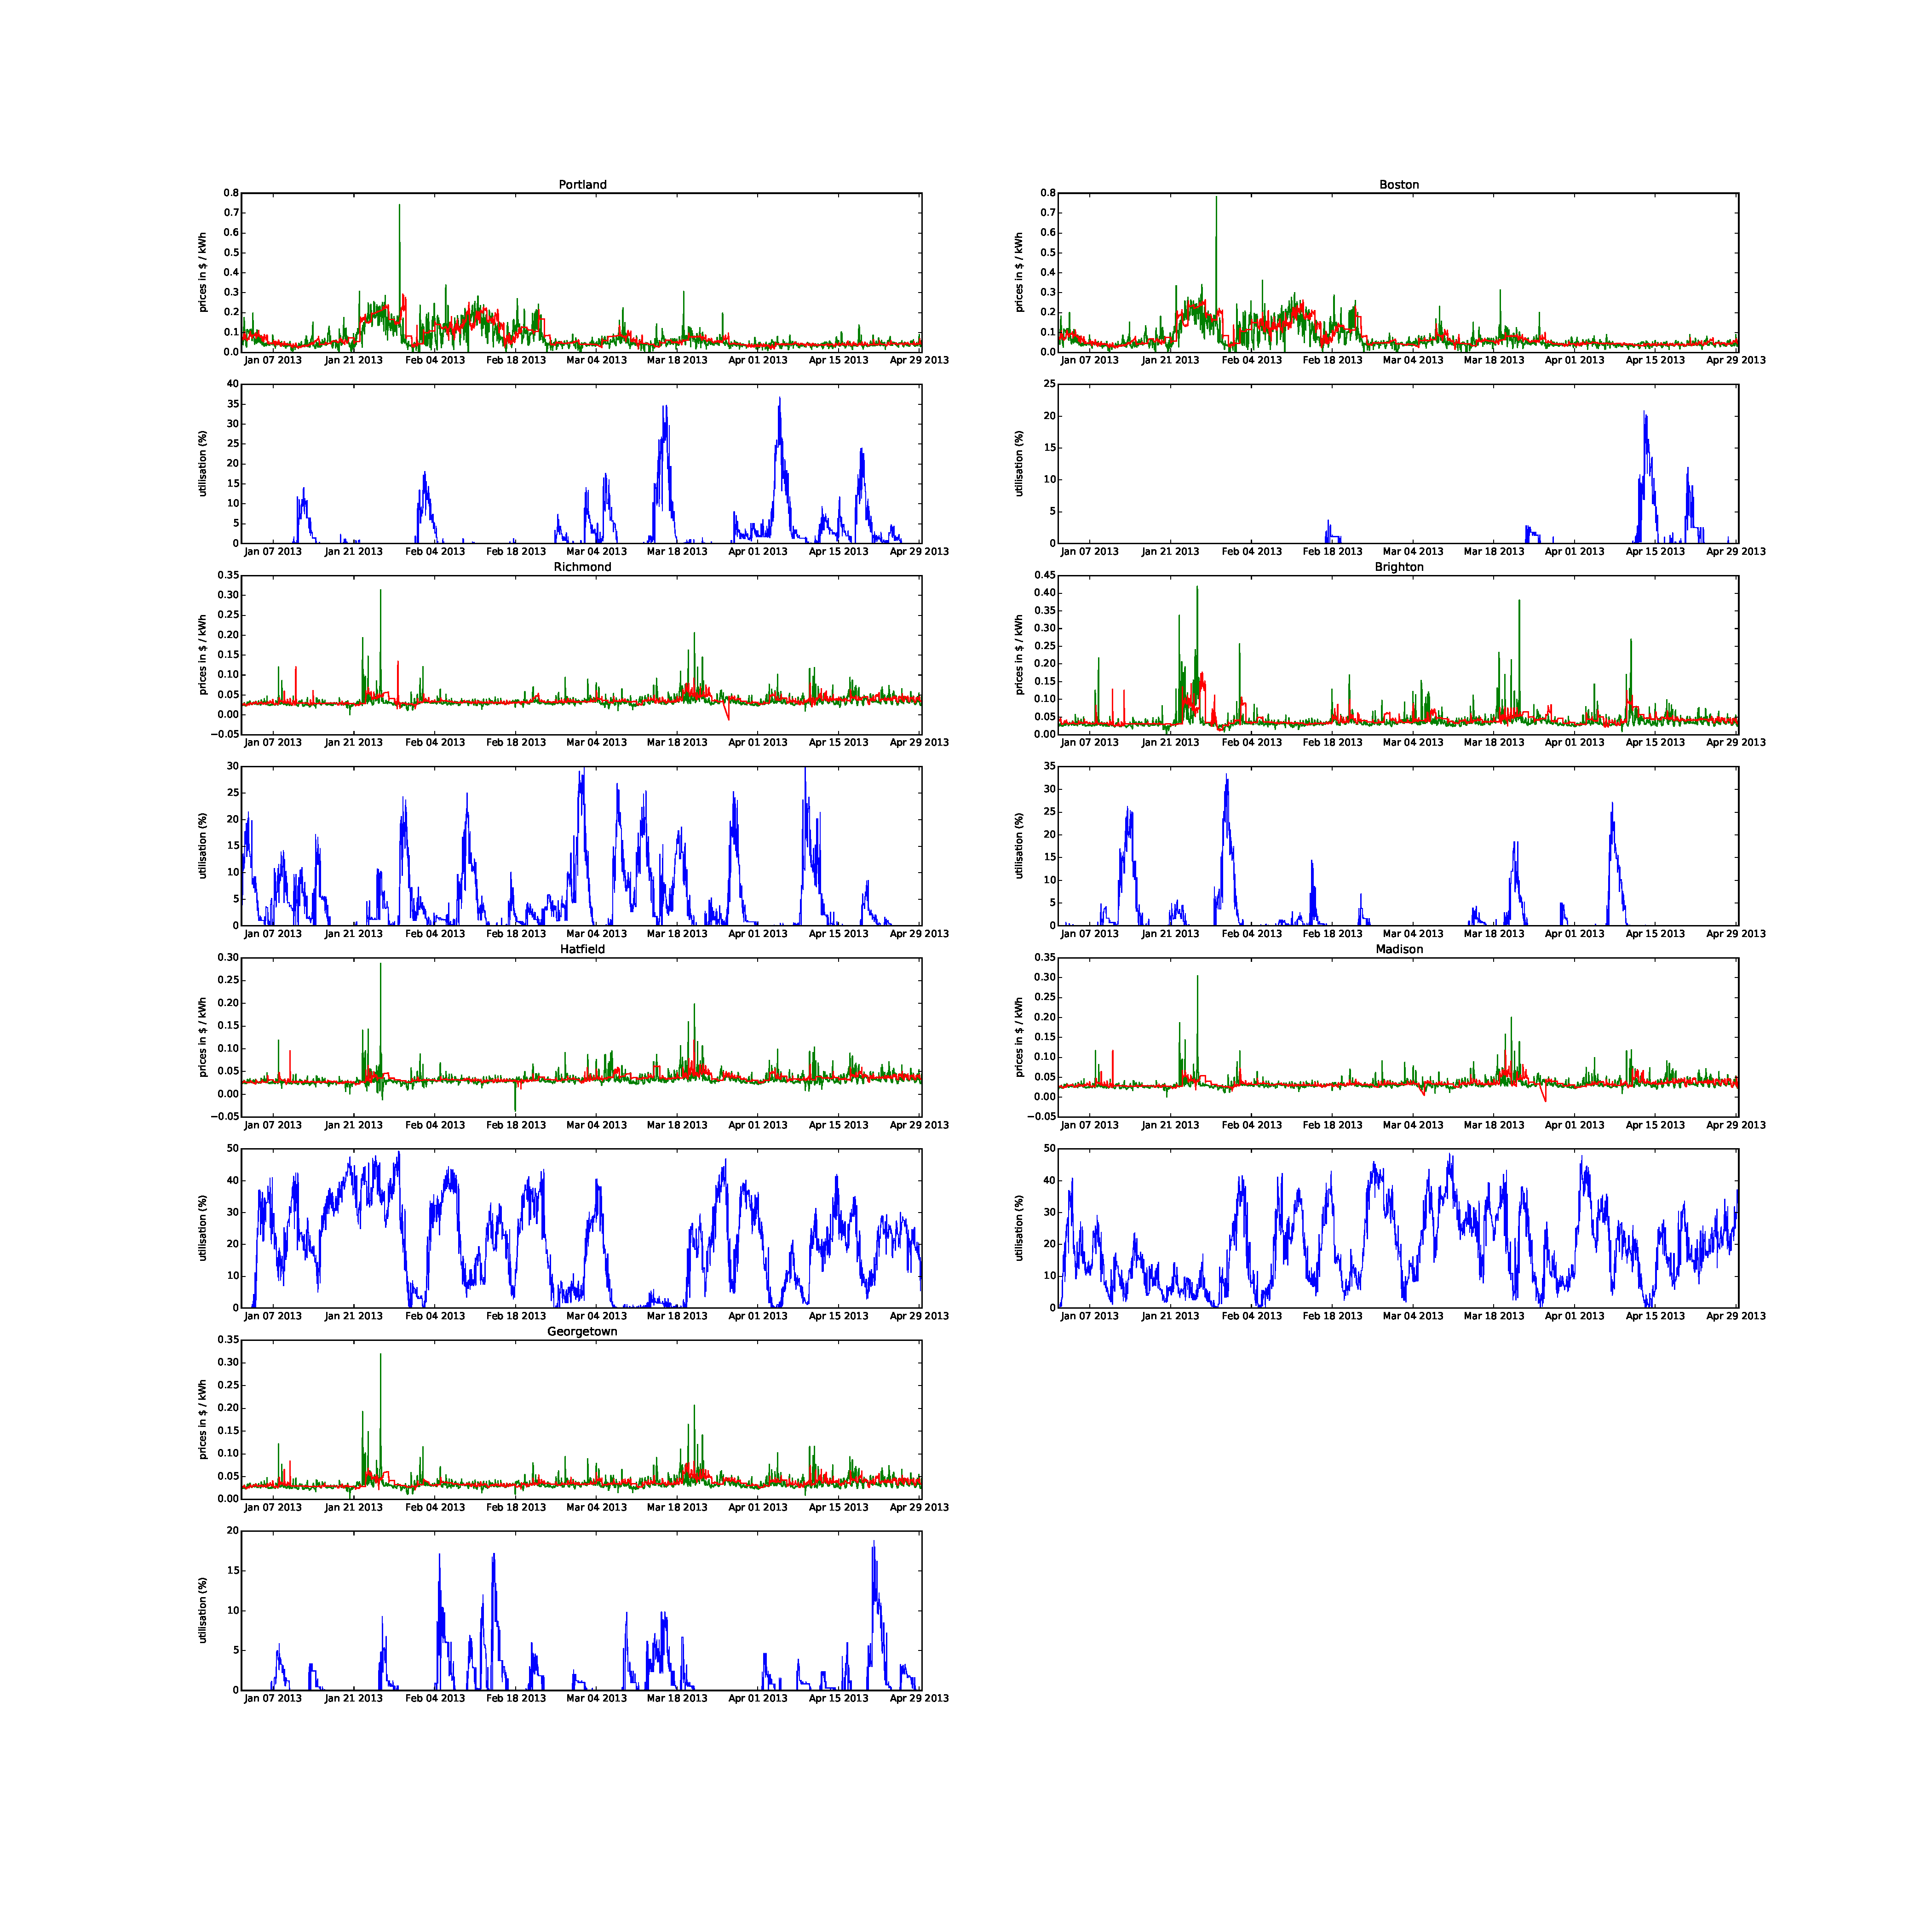
\includegraphics[width=1.60\textwidth]{figures/appendix_simulation_results/RT_Spring_scenario_3.pdf}
	\vspace*{-1.0in}
	\caption{Energy prices, energy price forecasts and utilization levels per location for simulation ``RT Spring'' and scheduler BCF\_F}
	\label{fig:app_RT_Spring_scenario_3}
\end{figure}

\begin{figure}[htbp]
	\centering
	\vspace*{-0.6in}
	\hspace*{-1.9in}
		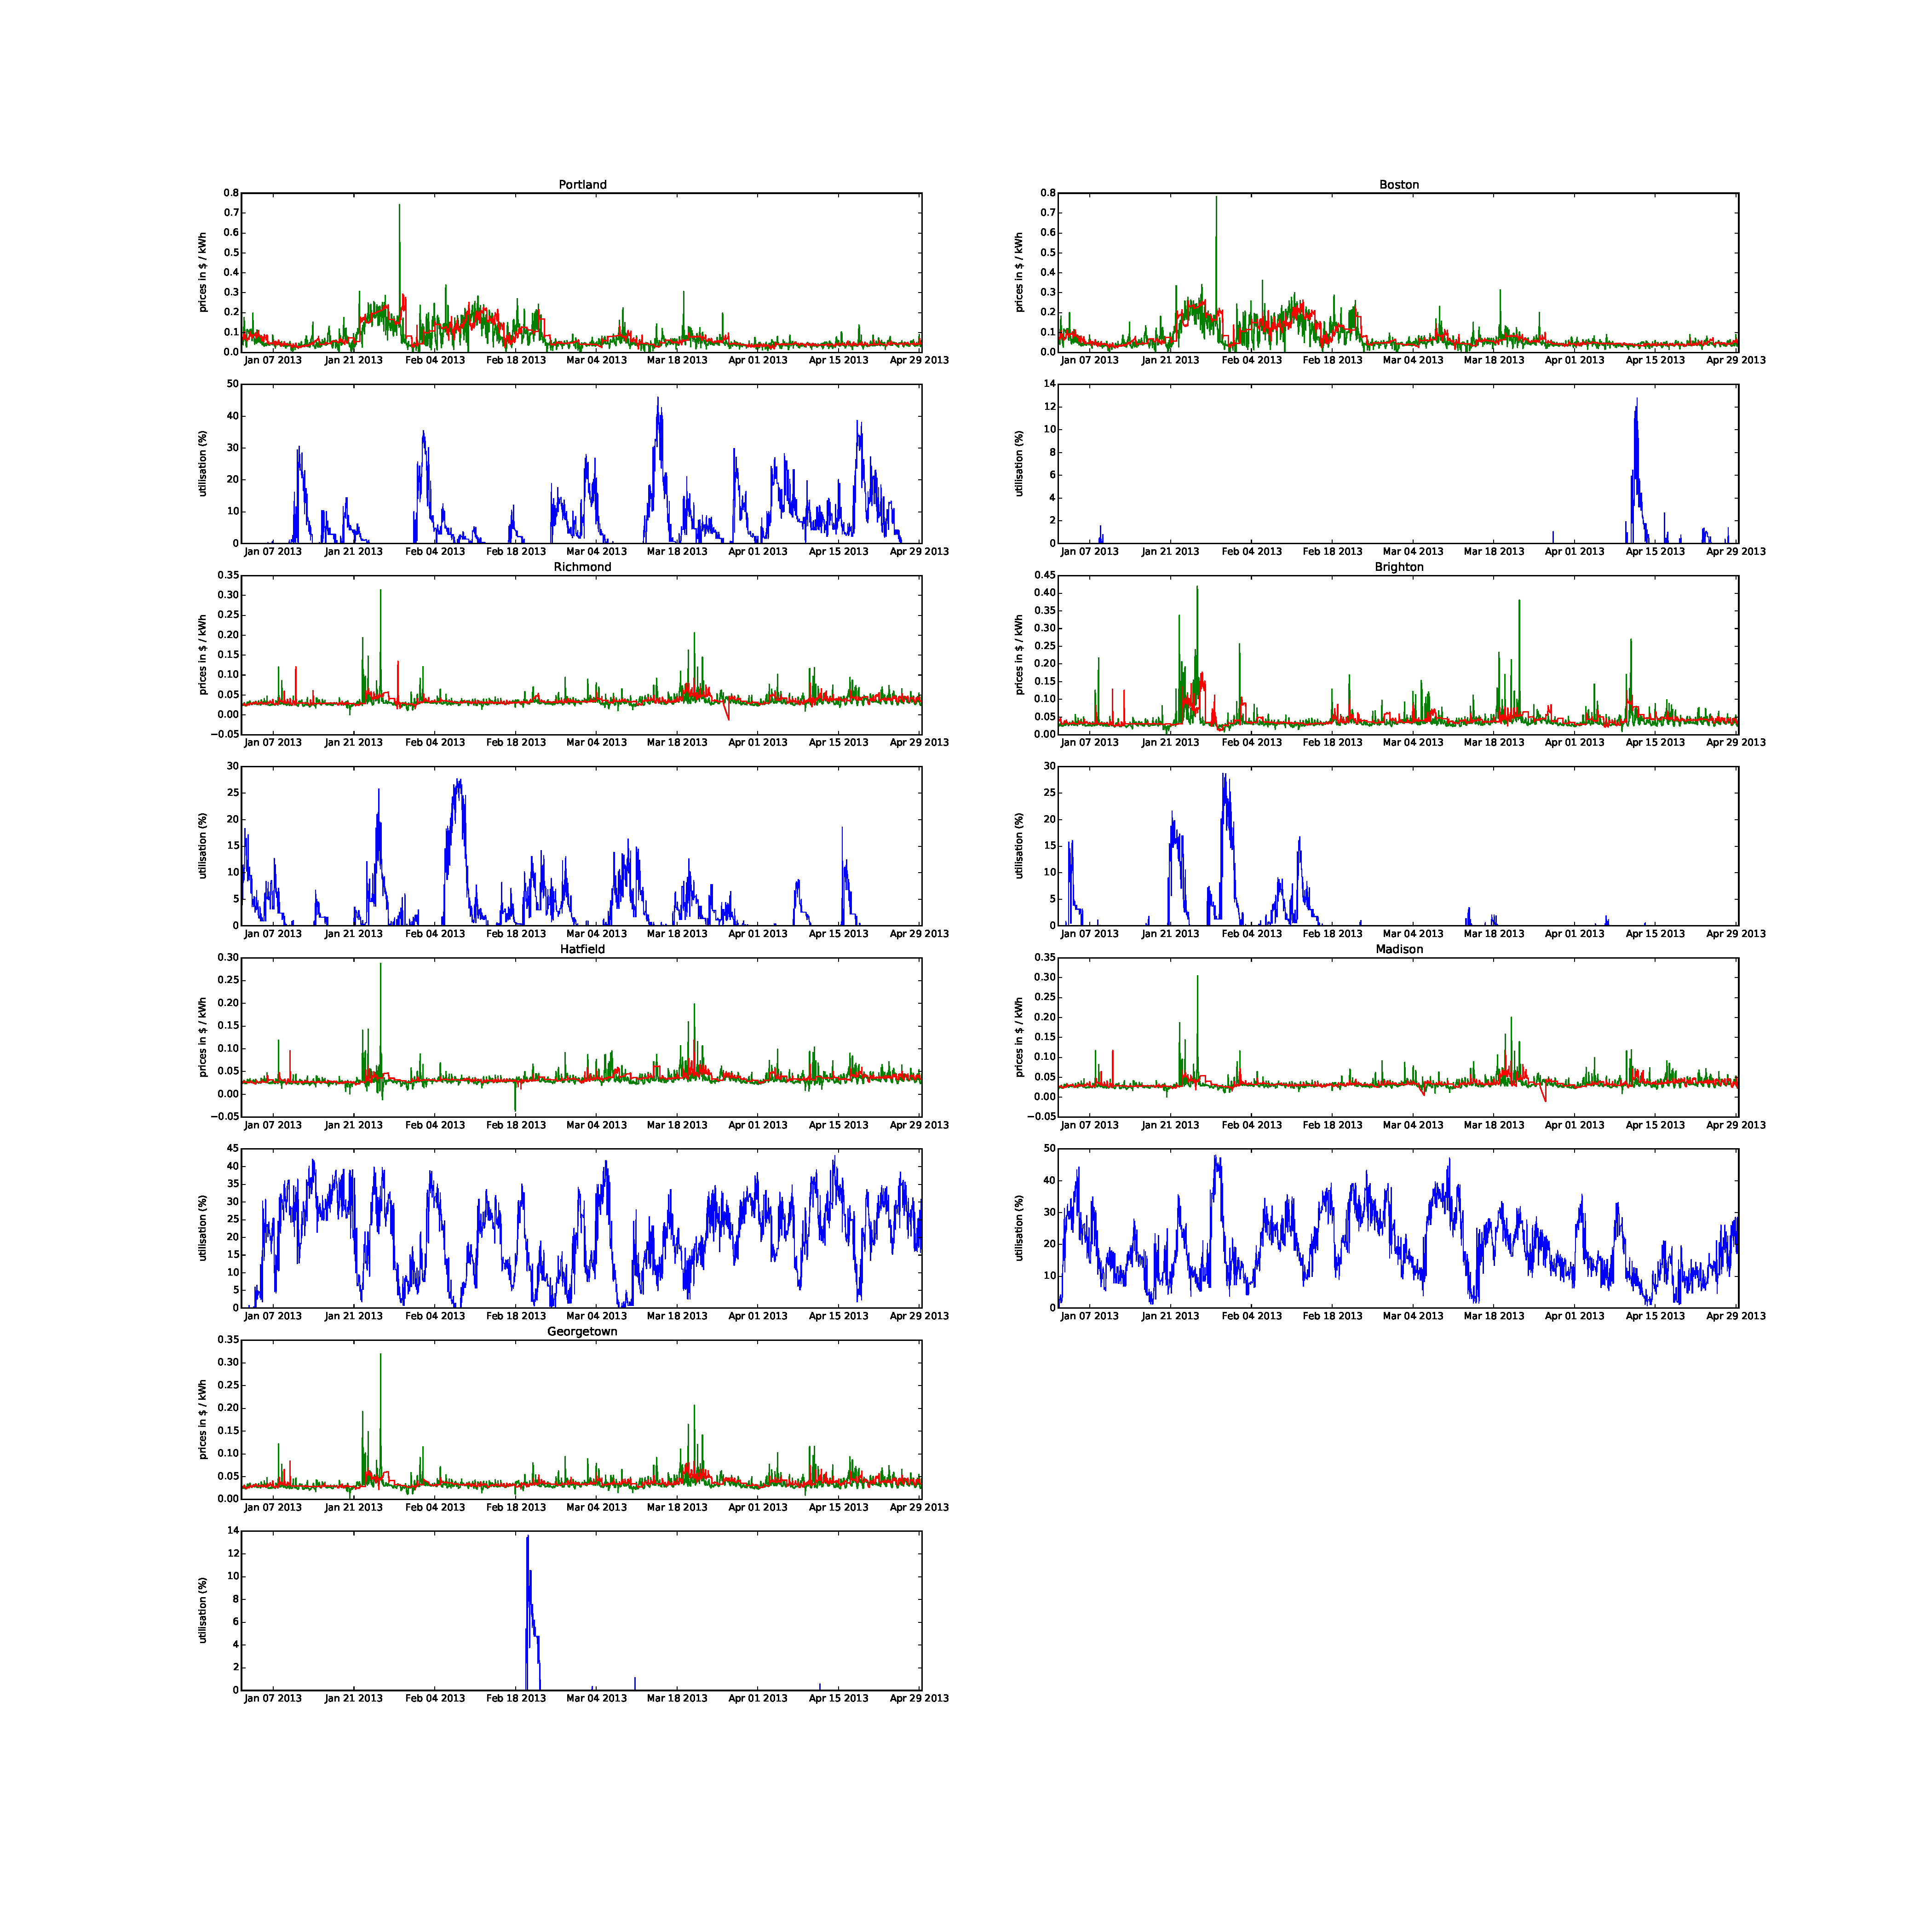
\includegraphics[width=1.60\textwidth]{figures/appendix_simulation_results/RT_Spring_scenario_4.pdf}
	\vspace*{-1.0in}
	\caption{Energy prices, energy price forecasts and utilization levels per location for simulation ``RT Spring'' and scheduler BCF\_IF}
	\label{fig:app_RT_Spring_scenario_4}
\end{figure}

\begin{figure}[htbp]
	\centering
	\vspace*{-0.6in}
	\hspace*{-1.4in}
		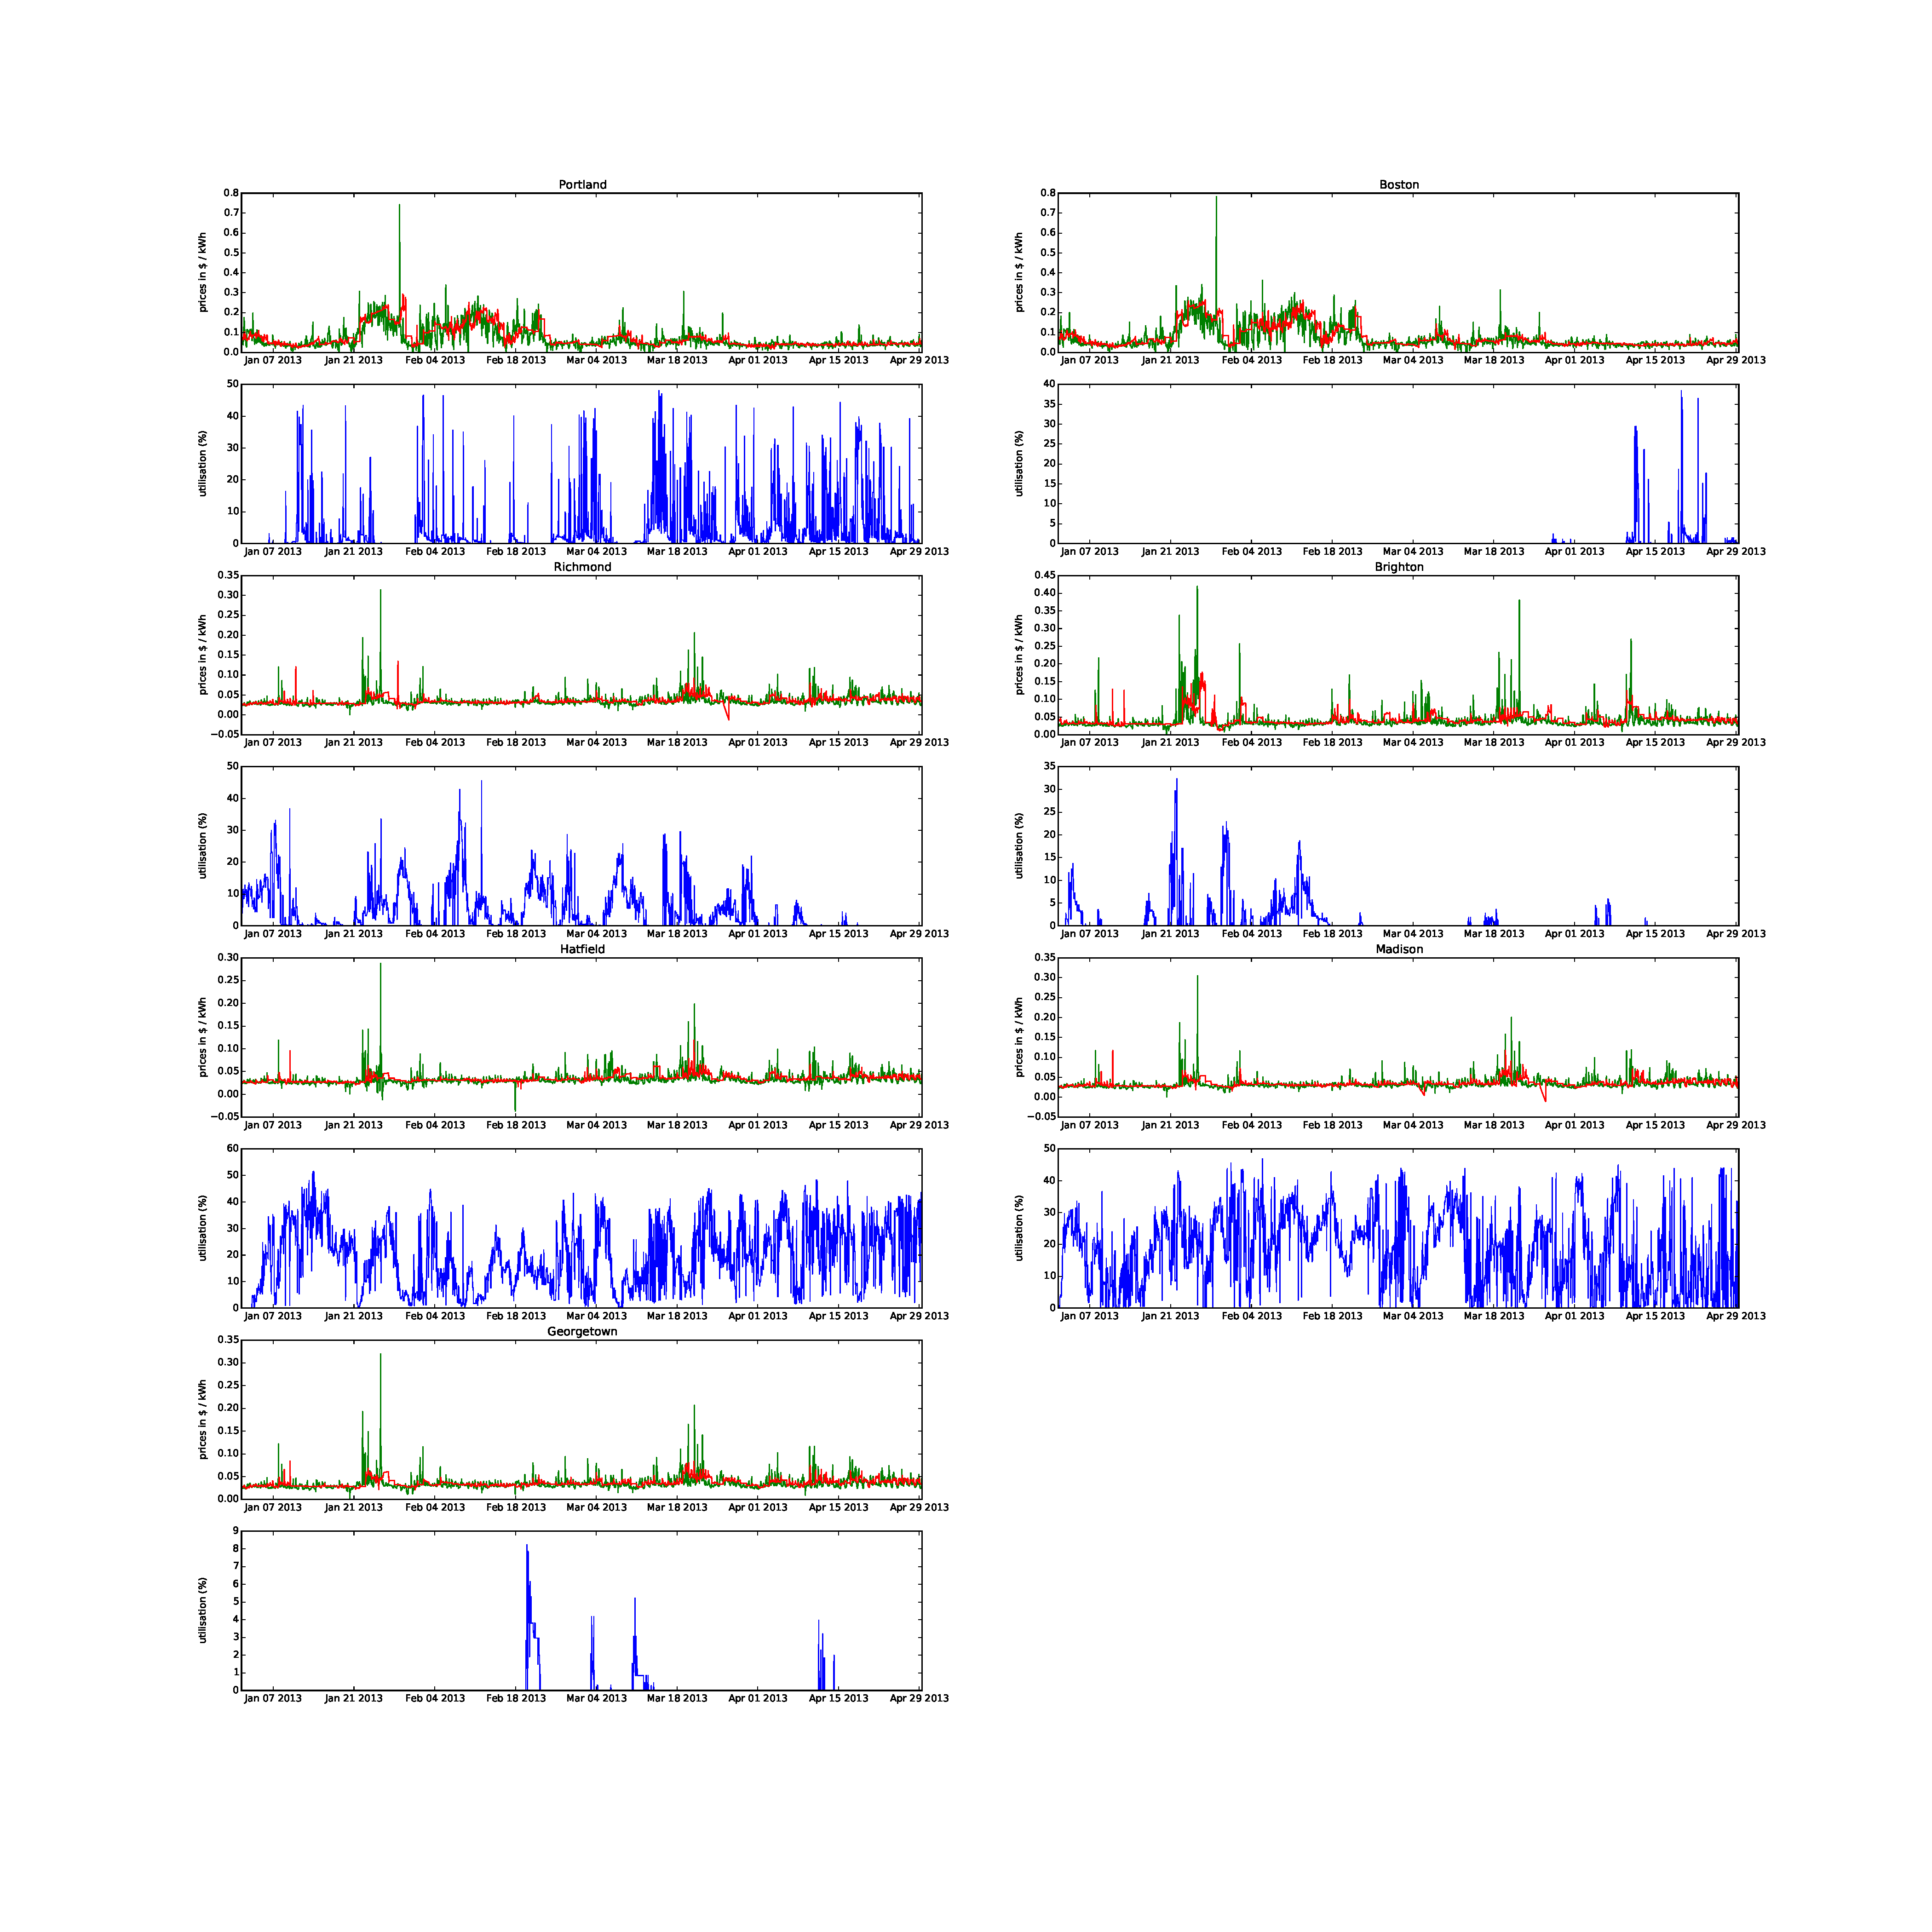
\includegraphics[width=1.60\textwidth]{figures/appendix_simulation_results/RT_Spring_scenario_5.pdf}
	\vspace*{-1.0in}
	\caption{Energy prices, energy price forecasts and utilization levels per location for simulation ``RT Spring'' and scheduler BCU\_M}
	\label{fig:app_RT_Spring_scenario_5}
\end{figure}

\begin{figure}[htbp]
	\centering
	\vspace*{-0.6in}
	\hspace*{-1.9in}
		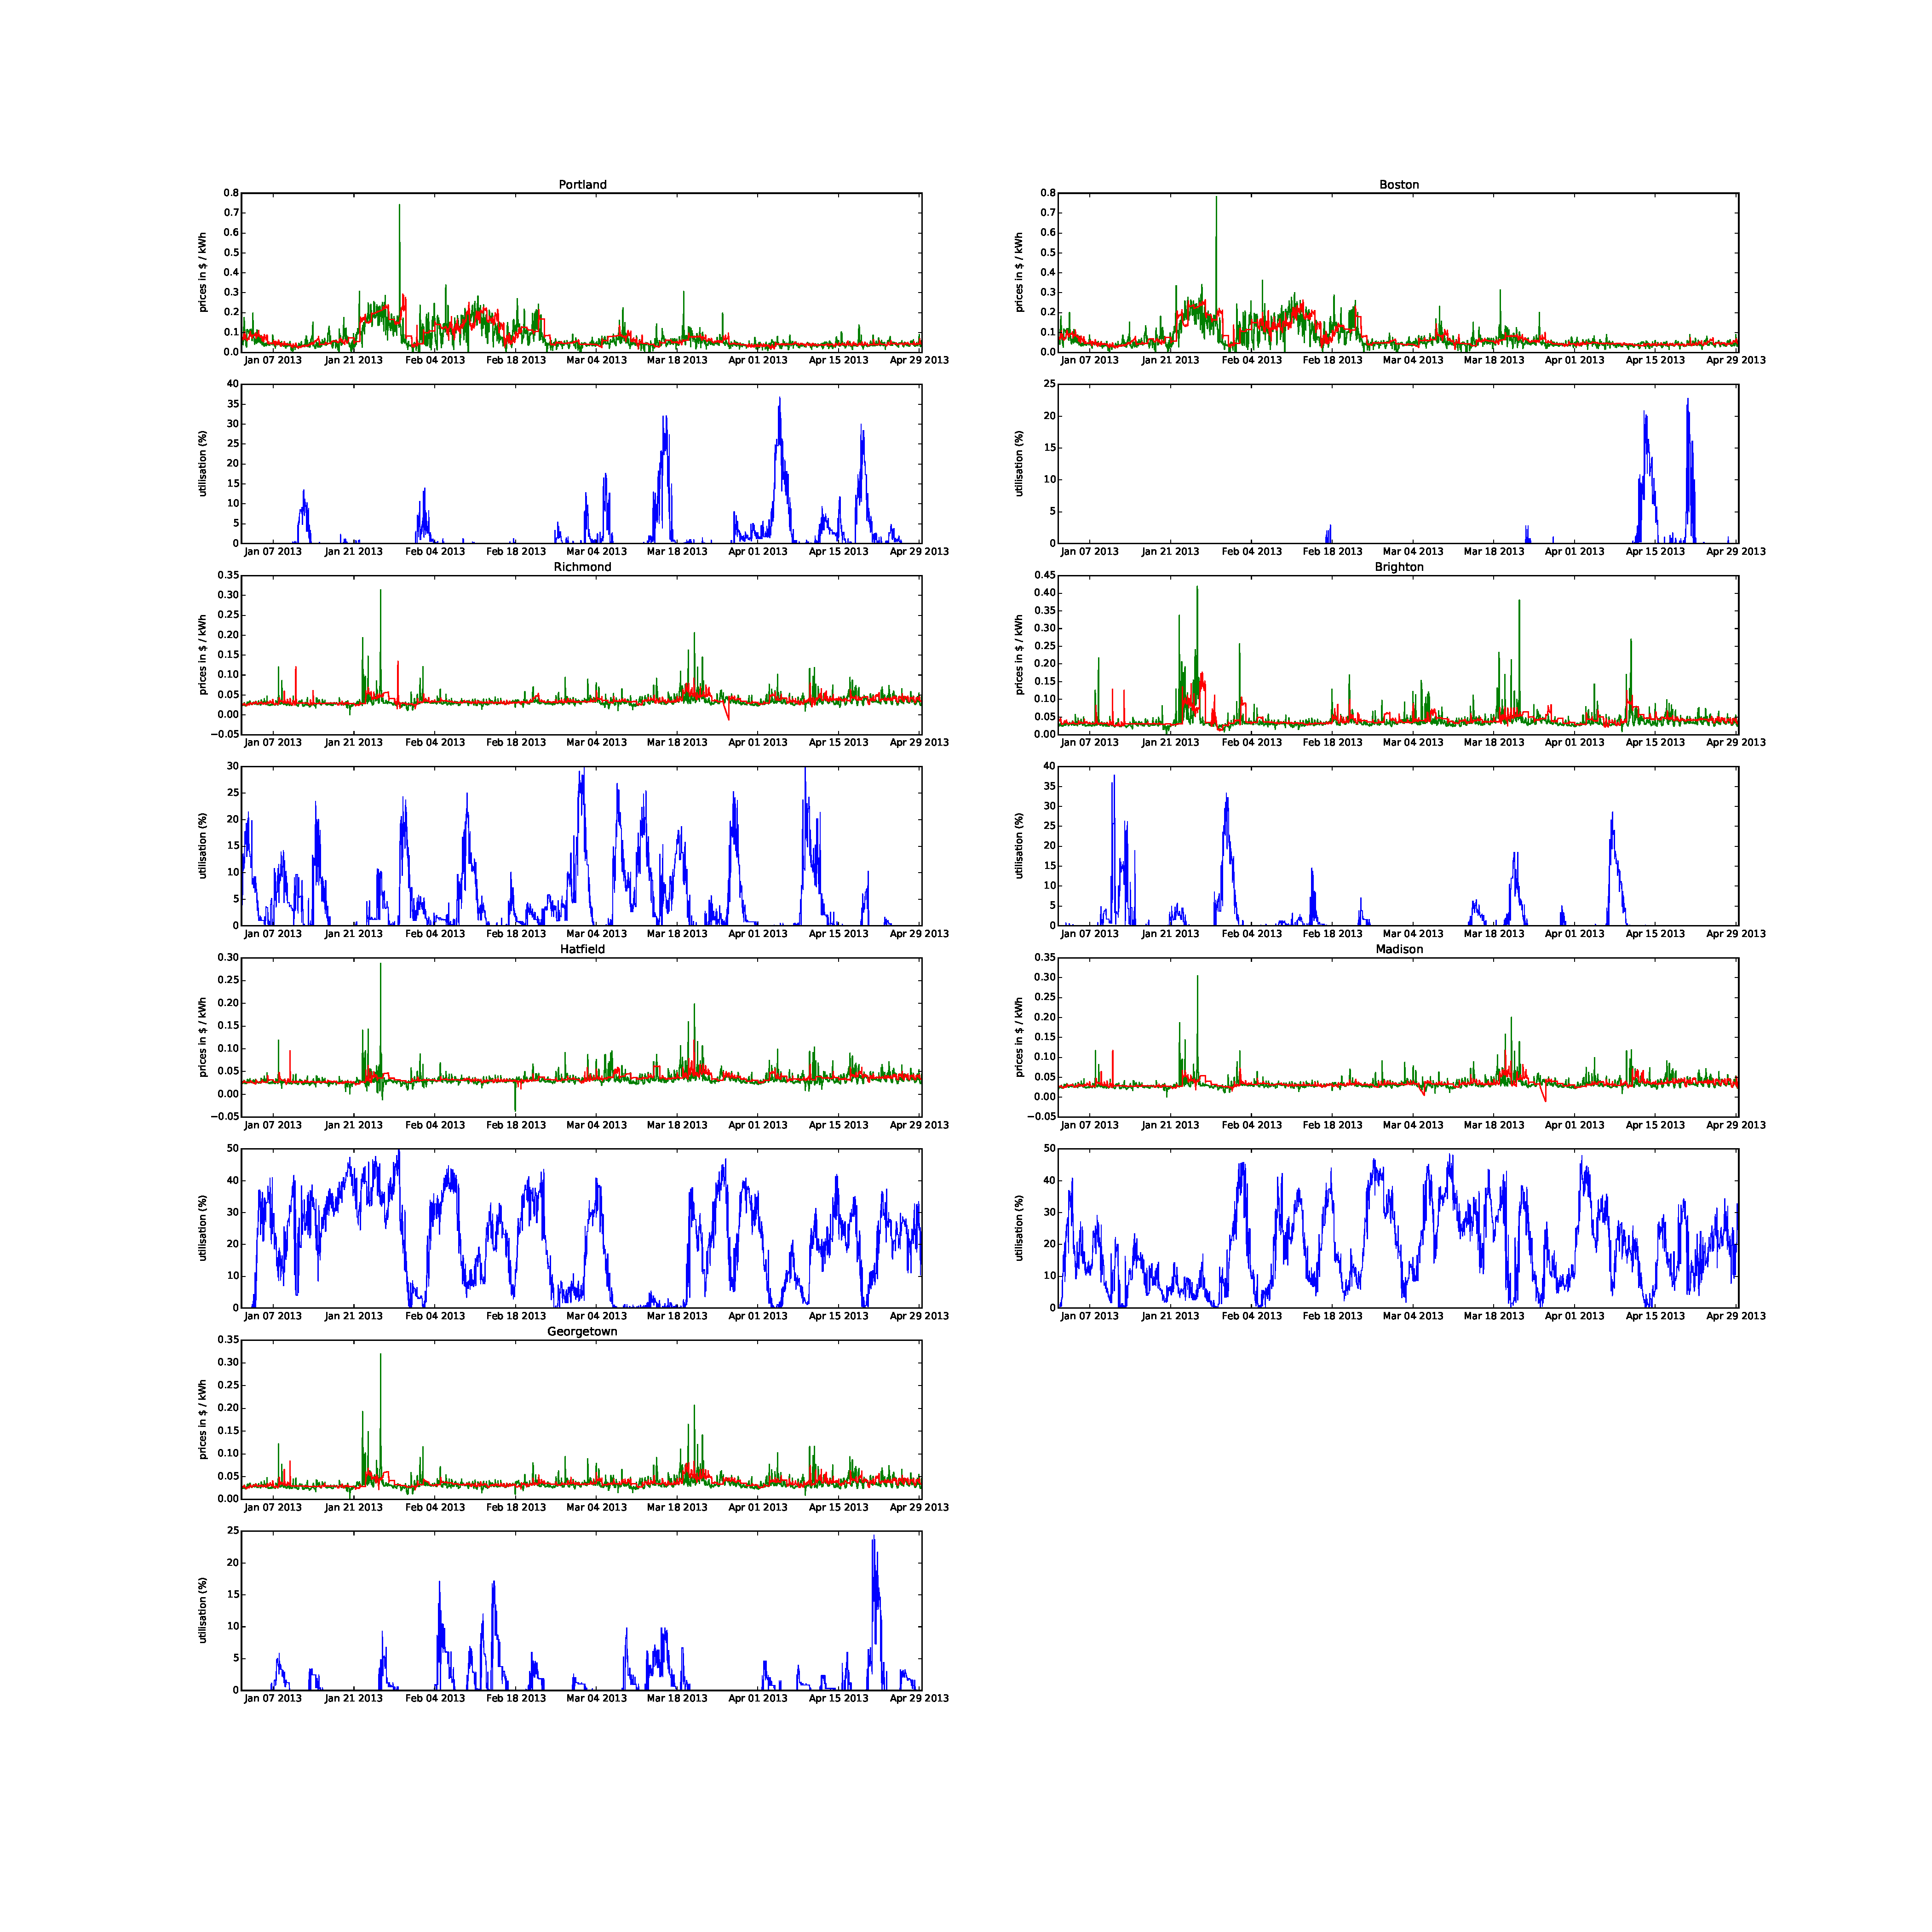
\includegraphics[width=1.60\textwidth]{figures/appendix_simulation_results/RT_Spring_scenario_6.pdf}
	\vspace*{-1.0in}
	\caption{Energy prices, energy price forecasts and utilization levels per location for simulation ``RT Spring'' and scheduler BCU\_MF}
	\label{fig:app_RT_Spring_scenario_6}
\end{figure}

\begin{figure}[htbp]
	\centering
	\vspace*{-0.6in}
	\hspace*{-1.4in}
		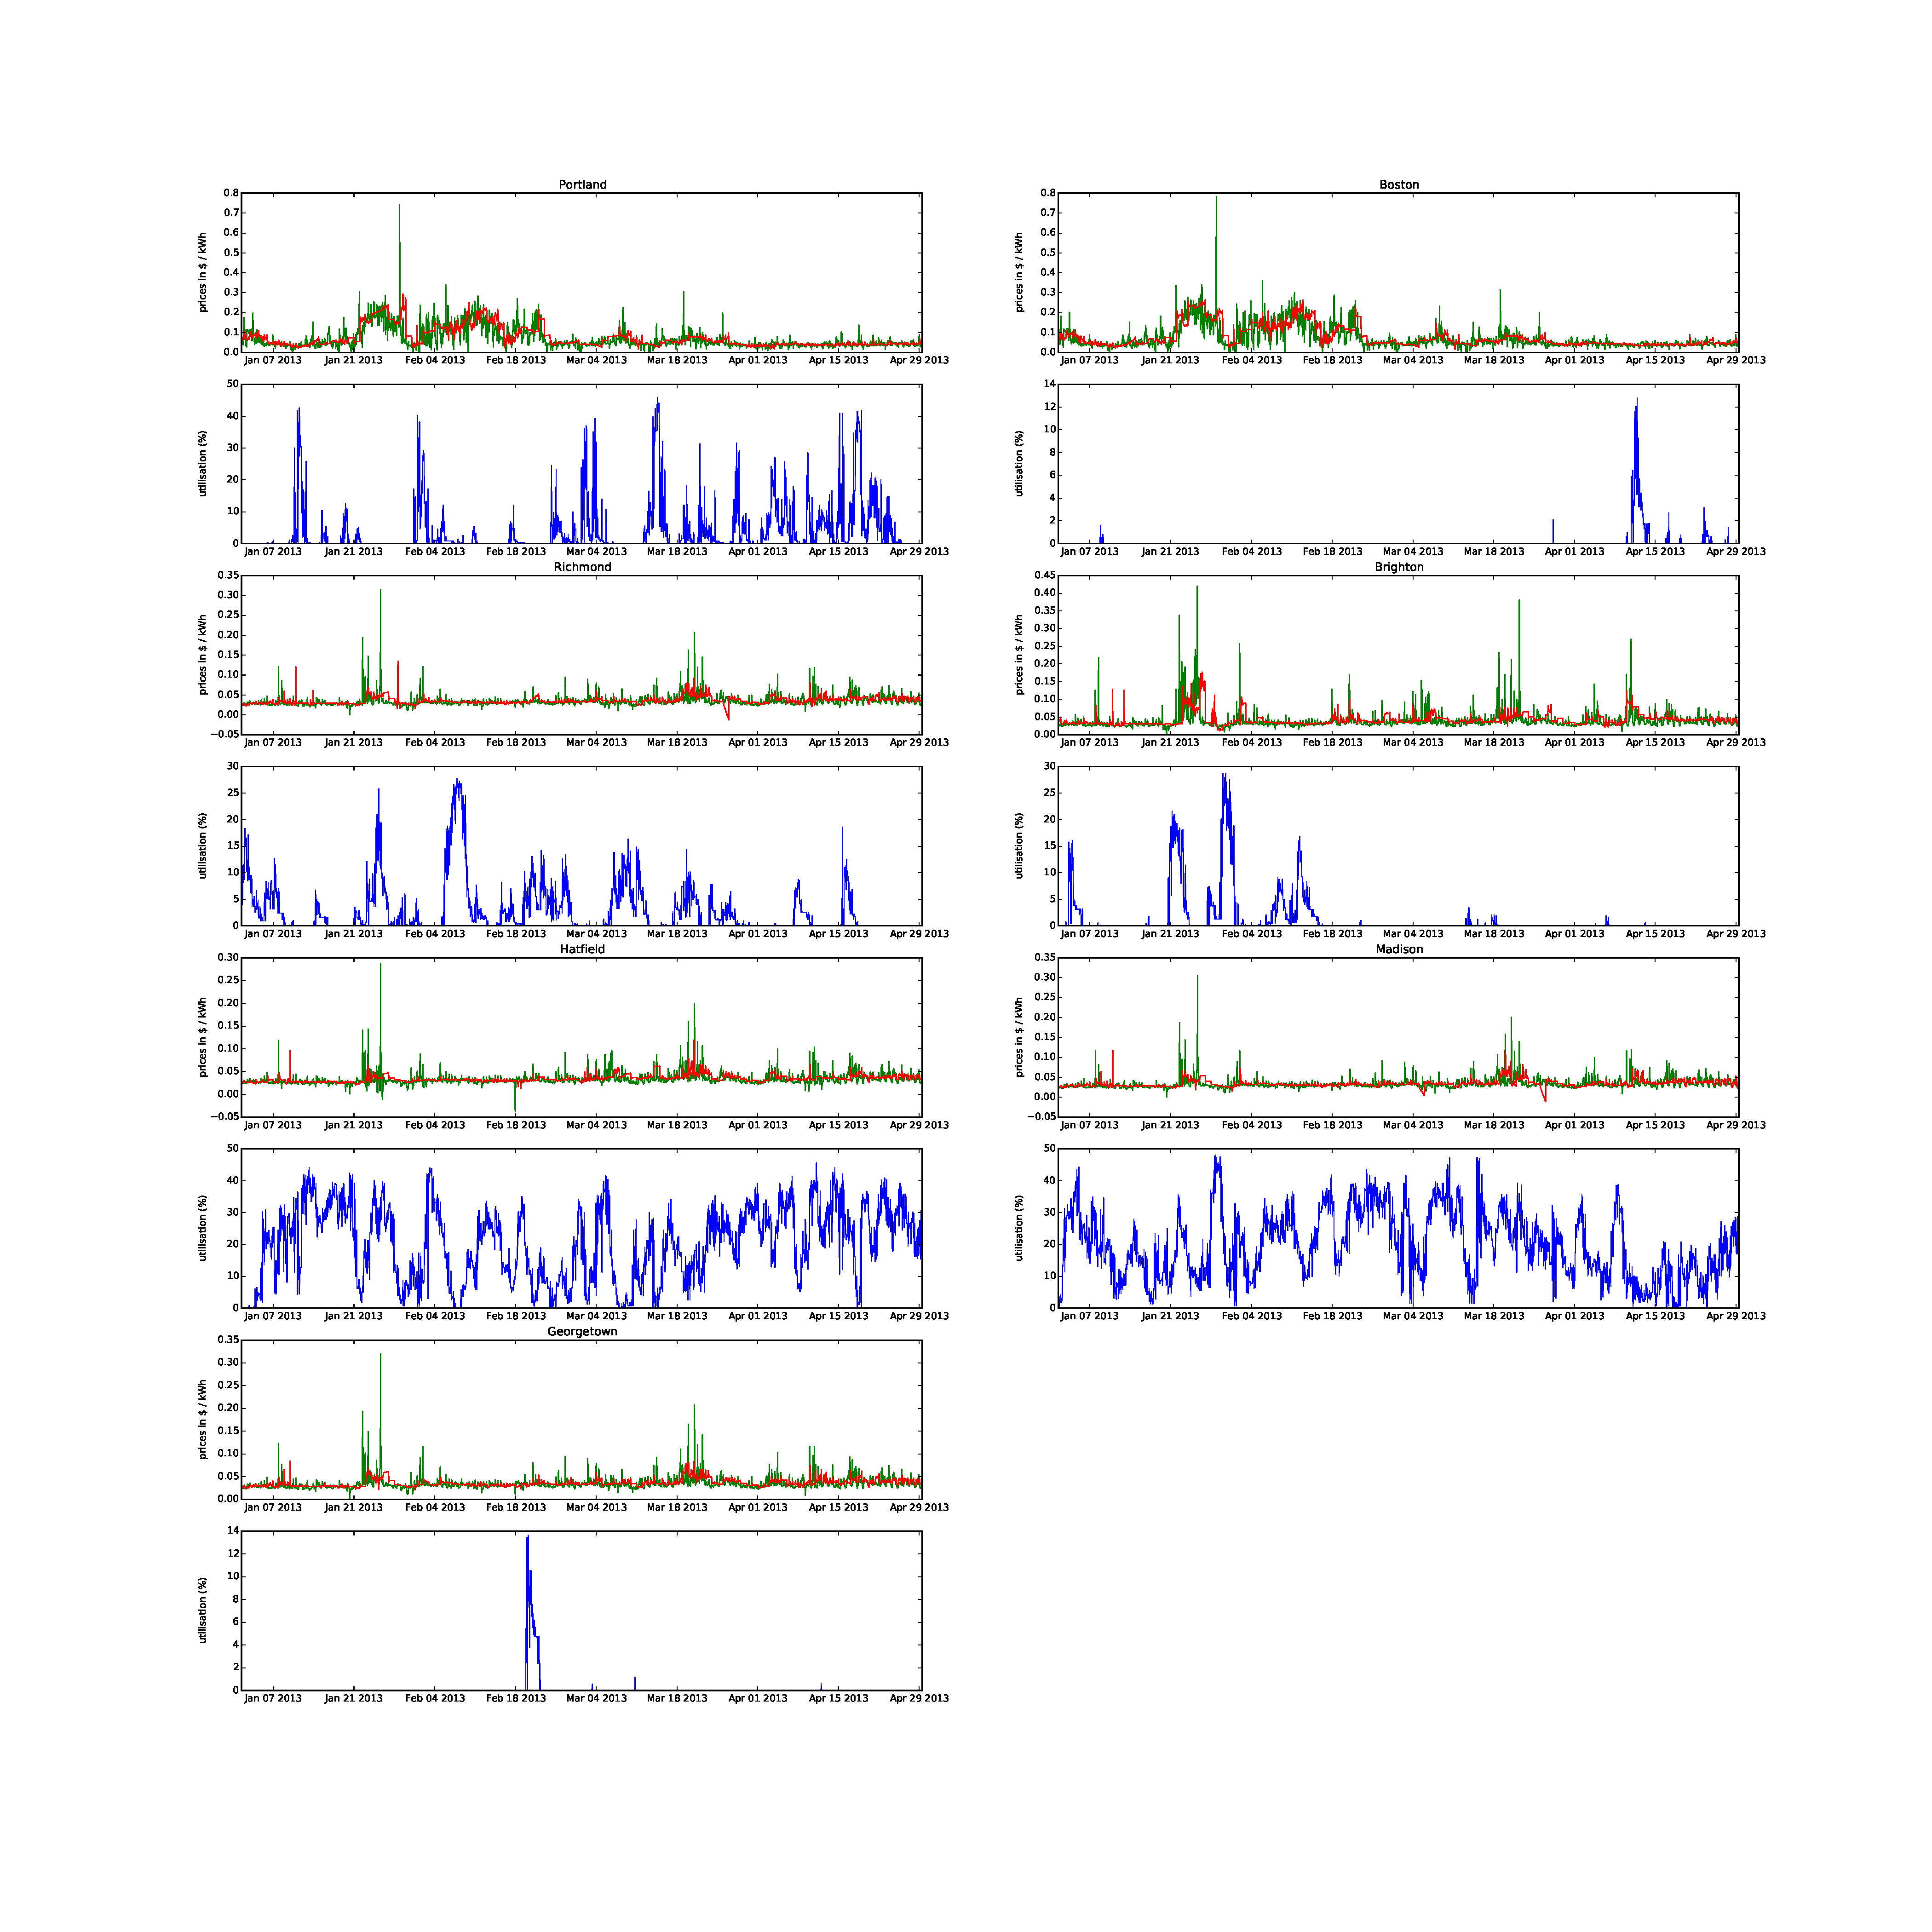
\includegraphics[width=1.60\textwidth]{figures/appendix_simulation_results/RT_Spring_scenario_7.pdf}
	\vspace*{-1.0in}
	\caption{Energy prices, energy price forecasts and utilization levels per location for simulation ``RT Spring'' and scheduler BCU\_MIF}
	\label{fig:app_RT_Spring_scenario_7}
\end{figure}


